\documentclass[aspectratio=169,10pt,t]{beamer}

\usepackage[T1]{fontenc}
\usepackage[utf8]{inputenc}
\usepackage{lmodern}
\usepackage{amsmath}
\usepackage{array}
\usepackage{booktabs}
\usepackage{colortbl}
\usepackage{graphicx}
\usepackage{tikz}
\usepackage{listings}
\usepackage{multicol}
\usepackage{microtype}
\usetikzlibrary{arrows.meta,positioning,shapes.geometric,calc,decorations.pathreplacing,fit,backgrounds,matrix}

\graphicspath{{figures/}{assets/}}

% ===== Official SGSMA 2026 template palette =====
\definecolor{ofbBlue}{HTML}{156082}
\definecolor{ofbRust}{HTML}{E97132}
\definecolor{ofbPlum}{HTML}{6A4C93}
\definecolor{ofbMoss}{HTML}{8A8F2F}
\definecolor{ofbRed}{HTML}{B23A48}
\definecolor{ofbInk}{HTML}{0E2841}
\definecolor{ofbSoft}{HTML}{F3F5F7}
\definecolor{ofbGreen}{HTML}{196B24}
\definecolor{ofbGold}{HTML}{E97132}
\definecolor{ofbViolet}{HTML}{A02B93}
\definecolor{ofbCanvas}{HTML}{FFFFFF}
\definecolor{ofbMuted}{HTML}{5B677A}
\definecolor{ofbLine}{HTML}{D9E1E8}
\definecolor{ofbNavy}{HTML}{0E2841}
\definecolor{sgsmaTeal}{HTML}{12695F}
\definecolor{sgsmaAqua}{HTML}{A8E6DF}
\definecolor{cardFill}{HTML}{F8FAFB}
\definecolor{cardBorder}{HTML}{CBD7DF}

% ===== Content-helper palette (carried from the technical deck, used by tikz) =====
\definecolor{Navy}{HTML}{071B33}
\definecolor{Ink}{HTML}{17212B}
\definecolor{Muted}{HTML}{5B6773}
\definecolor{Cyan}{HTML}{13A8A8}
\definecolor{Blue}{HTML}{165DFF}
\definecolor{Green}{HTML}{2E7D32}
\definecolor{Orange}{HTML}{F08A24}
\definecolor{Red}{HTML}{B3261E}
\definecolor{Paper}{HTML}{F6F8FB}
\definecolor{Line}{HTML}{D9E1EA}
\definecolor{SoftBlue}{HTML}{EAF2FF}
\definecolor{SoftCyan}{HTML}{E7F8F8}
\definecolor{SoftGreen}{HTML}{ECF6EE}
\definecolor{SoftOrange}{HTML}{FFF2E3}
\definecolor{SoftRed}{HTML}{FCEBEC}

\newcommand{\sgsmaTitleBg}{figures/sgsma_title_bg.png}
\newcommand{\sgsmaDividerBg}{figures/sgsma_divider_bg.png}
\newcommand{\sgsmaContentBg}{figures/sgsma_content_bg.png}

\usetheme{default}
\usecolortheme[named=ofbBlue]{structure}
\setbeamertemplate{navigation symbols}{}
\setbeamercolor{normal text}{fg=ofbInk,bg=ofbCanvas}
\setbeamercolor{title}{fg=white,bg=ofbNavy}
\setbeamercolor{frametitle}{fg=ofbInk,bg=ofbCanvas}
\setbeamercolor{block title}{fg=white,bg=sgsmaTeal}
\setbeamercolor{block body}{fg=ofbInk,bg=cardFill}
% palette-consistent alert/example blocks (the technical deck uses all three types)
\setbeamercolor{block title example}{fg=white,bg=ofbGreen}
\setbeamercolor{block body example}{fg=ofbInk,bg=ofbGreen!8}
\setbeamercolor{block title alerted}{fg=white,bg=ofbRust}
\setbeamercolor{block body alerted}{fg=ofbInk,bg=ofbRust!10}
\setbeamercolor{footline}{fg=white}
\setbeamerfont{frametitle}{family=\rmfamily,series=\mdseries,size=\fontsize{16.5}{19}\selectfont}
\setbeamerfont{title}{family=\rmfamily,series=\mdseries,size=\Large}
\setbeamerfont{block title}{series=\bfseries,size=\small}
\setbeamersize{text margin left=8mm,text margin right=8mm}
\usebackgroundtemplate{\includegraphics[width=\paperwidth,height=\paperheight]{\sgsmaContentBg}}
\setbeamertemplate{itemize item}{\raisebox{0.15ex}{\scriptsize\textcolor{ofbBlue}{$\bullet$}}}
\setbeamertemplate{itemize subitem}{\raisebox{0.1ex}{\tiny\textcolor{ofbGold}{$\bullet$}}}
\setbeamertemplate{enumerate item}{\textcolor{ofbBlue}{\insertenumlabel.}}
\setbeamertemplate{blocks}[rounded][shadow=false]
\setbeamertemplate{frametitle}{%
  \vspace{0.33cm}
  \hspace{8mm}\begin{minipage}[t]{0.76\paperwidth}
    \raggedright\hyphenpenalty=10000\exhyphenpenalty=10000
    \usebeamerfont{frametitle}\color{ofbInk}\insertframetitle
  \end{minipage}\par
  \vspace{0.12cm}
}
\setbeamertemplate{footline}{%
  \begin{tikzpicture}[remember picture,overlay]
    \node[anchor=south, text=white, font=\tiny] at ([xshift=-0.08\paperwidth,yshift=0.13cm]current page.south) {\insertframenumber/\inserttotalframenumber};
    \node[anchor=south, text=white, font=\tiny\itshape] at ([xshift=0.10\paperwidth,yshift=0.13cm]current page.south) {\insertsection};
  \end{tikzpicture}%
  \vspace*{0.84cm}%
}

% ===== Content-helper macros (carried from the technical deck) =====
\newcommand{\code}[1]{\texttt{\footnotesize #1}}
\newcommand{\smallcode}[1]{\texttt{\scriptsize #1}}
\newcommand{\pill}[2]{%
  \tikz[baseline=(n.base)] \node[rounded corners=8pt,fill=#1!13,draw=#1,inner xsep=6pt,inner ysep=2pt] (n) {\scriptsize\bfseries #2};%
}
\newcommand{\metricbox}[3]{%
  \begin{tikzpicture}
    \node[rounded corners=5pt,draw=#1,fill=#1!9,minimum width=2.7cm,minimum height=1.25cm,align=center] {
      {\Large\bfseries #2}\\[-1mm]{\scriptsize #3}
    };
  \end{tikzpicture}
}
\newcommand{\stagebox}[3]{%
  \tikz[baseline=(n.base)] \node[rounded corners=4pt,draw=#1,fill=#1!9,inner xsep=5pt,inner ysep=3pt,text width=#2,align=center,font=\scriptsize] (n) {#3};%
}

% ===== Official template helper macros =====
\newcommand{\artifact}[1]{\vspace{0.20em}{\tiny\color{ofbMuted}Source: \texttt{#1}}}
\newcommand{\callout}[1]{%
  \vspace{0.25em}\noindent
  \begin{tikzpicture}
    \node[draw=cardBorder,fill=cardFill,rounded corners=2pt,line width=0.45pt,inner xsep=7pt,inner ysep=6pt,text width=0.94\linewidth,align=left] {\small #1};
    \draw[sgsmaTeal, line width=1.3pt] ([xshift=0.5pt,yshift=-0.5pt]current bounding box.north west) -- ([xshift=0.5pt,yshift=0.5pt]current bounding box.south west);
  \end{tikzpicture}%
  \vspace{0.15em}
}
\newcommand{\tagpill}[2]{%
  \tikz[baseline=(x.base)]\node[inner xsep=5pt,inner ysep=2pt,rounded corners=2pt,fill=#1!12,draw=#1,text=ofbInk,font=\scriptsize\bfseries] (x) {#2};%
}
\newcommand{\statcard}[3]{%
\begin{tikzpicture}
\node[draw=cardBorder,fill=cardFill,rounded corners=2pt,line width=0.55pt,inner sep=7pt,text width=0.86\linewidth,minimum height=1.18cm,align=left] {
{\scriptsize\bfseries\color{ofbMuted}#2}\\[0.10em]
{\Large\bfseries\color{#1}#3}
};
\draw[#1, line width=1.5pt] ([xshift=0.5pt,yshift=-0.5pt]current bounding box.north west) -- ([xshift=0.5pt,yshift=0.5pt]current bounding box.south west);
\end{tikzpicture}}
\newcommand{\sectionframe}[3]{%
\begin{frame}[plain]
\begin{tikzpicture}[remember picture,overlay]
  \node[anchor=center] at (current page.center) {\includegraphics[width=\paperwidth,height=\paperheight]{\sgsmaDividerBg}};
  \node[anchor=east, text=white, align=right, font=\fontsize{27}{32}\selectfont\rmfamily, text width=0.64\paperwidth] at ([xshift=-0.075\paperwidth,yshift=0.25cm]current page.east) {\hyphenpenalty=10000\exhyphenpenalty=10000\pretolerance=10000\tolerance=10000\emergencystretch=3em #2};
  \node[anchor=east, text=white, align=right, font=\large, text width=0.62\paperwidth] at ([xshift=-0.075\paperwidth,yshift=-1.00cm]current page.east) {\hyphenpenalty=10000\exhyphenpenalty=10000 #3};
\end{tikzpicture}
\end{frame}}

% ===== Code listing style (carried from the technical deck) =====
\lstdefinestyle{sgcode}{
  basicstyle=\ttfamily\scriptsize,
  keywordstyle=\color{ofbBlue}\bfseries,
  commentstyle=\color{ofbMuted},
  stringstyle=\color{ofbGreen},
  breaklines=true,
  columns=fullflexible,
  keepspaces=true,
  frame=single,
  rulecolor=\color{ofbLine},
  backgroundcolor=\color{ofbSoft},
  showstringspaces=false
}
\lstset{style=sgcode}

\title[SGSMA 2026]{Physics-Informed PMU Event Detection and Localization}
\subtitle{A buildable recipe for the final SGSMA submission method}
\author{Jorge Luis Mayorga Taborda, Yessica Africano Rodriguez}
\institute{Universidad de los Andes}
\date{June 1--4, 2026}

\begin{document}

{
\setbeamertemplate{footline}{}
\begin{frame}[plain]
\begin{tikzpicture}[remember picture,overlay]
  \node[anchor=center] at (current page.center) {\includegraphics[width=\paperwidth,height=\paperheight]{\sgsmaTitleBg}};
  \node[anchor=west, text=white, align=left, font=\fontsize{18}{23}\selectfont\rmfamily\itshape, text width=0.72\paperwidth] at ([xshift=0.056\paperwidth,yshift=-0.45cm]current page.west) {
    Physics-Informed PMU Event\\[-0.05em]
    Detection and Localization
  };
  \node[anchor=west, text=white, align=left, font=\scriptsize\itshape, text width=0.72\paperwidth] at ([xshift=0.068\paperwidth,yshift=-1.75cm]current page.west) {
    Jorge Luis Mayorga Taborda, Yessica Africano Rodriguez
  };
  \node[anchor=west, text=white, align=left, font=\tiny, text width=0.66\paperwidth] at ([xshift=0.068\paperwidth,yshift=-2.14cm]current page.west) {
    Universidad de los Andes \quad | \quad SGSMA 2026
  };
\end{tikzpicture}
\end{frame}
}



% -------------------------------------------------------------------
\begin{frame}{Method overview}
\small
\begin{columns}[T,totalwidth=\textwidth]
\begin{column}{0.48\textwidth}
\begin{block}{Pipeline}
\begin{enumerate}
  \item Convert raw PMU waveforms into physics-aware features.
  \item Use a hierarchical ExtraTrees classifier to identify event type.
  \item Route each event to a specialized BUS, LINE, or PMU localizer.
  \item Produce the challenge CSV output at timestamp resolution.
\end{enumerate}
\end{block}
\end{column}
\begin{column}{0.48\textwidth}
\begin{exampleblock}{Reimplementation target}
The method can be rebuilt from PMU windows, feature definitions, ExtraTrees models, and typed localization routes.
\end{exampleblock}
\begin{alertblock}{Submission boundary}
The submitted route is SGMS: physics-informed features, hierarchical ExtraTrees, and typed dynamic localizers. RAW-label-tuned and oracle branches are excluded from inference.
\end{alertblock}
\end{column}
\end{columns}
\end{frame}

% -------------------------------------------------------------------

% -------------------------------------------------------------------
\section{Problem and Data}
\sectionframe{}{Problem and Data}{PMU streams, event labels, and the prediction contract}


% -------------------------------------------------------------------
\begin{frame}{Task, event labels, and outputs}
\small
\begin{columns}[T,totalwidth=\textwidth]
\begin{column}{0.45\textwidth}
\begin{block}{Input}
Eight synchronized PMU CSV files: one per observed bus, about 90 min at 30 fps, with voltage/current phasors, frequency, ROCOF, \code{DATA\_PRESENT}, and hidden or blank \code{Event}.
\end{block}
\begin{alertblock}{Output}
\code{TIMESTAMP}, \code{Bus}, \code{Predicted\_Event}, and \code{Predicted\_Location}.
\end{alertblock}
\end{column}
\begin{column}{0.51\textwidth}
\centering
\scriptsize
\renewcommand{\arraystretch}{0.85}
\setlength{\tabcolsep}{3.5pt}
\begin{tabular}{clp{0.46\textwidth}}
\toprule
\textbf{Label} & \textbf{Name} & \textbf{Meaning}\\
\midrule
0 & normal & no disturbance or major data issue\\
1 & fault & fast, strong voltage disturbance\\
2 & line outage & current redistribution without fault-level voltage collapse\\
3 & generation & frequency/ROCOF and power-proxy shift\\
4 & load & sustained current and power change\\
5 & missing & data loss without physical evidence\\
6 & missing + physical & missing data plus physical event\\
7 & bad data & isolated inconsistent sensor/channel\\
8 & unknown & mixed physical evidence not explained by 1--4\\
\bottomrule
\end{tabular}
\end{column}
\end{columns}
\vspace{-3mm}
{\footnotesize\callout{\textbf{Decision structure:} detection, event classification, and localization are coupled, not one flat label.}}
\end{frame}

\iffalse
\begin{frame}{Challenge task}
\small
\begin{columns}[T,totalwidth=\textwidth]
\begin{column}{0.47\textwidth}
\begin{block}{Input}
Official package: eight synchronized PMU CSV files:
\begin{itemize}
  \item one file per observed bus,
  \item about 90 min at 30 fps,
  \item voltage/current phasors, frequency, ROCOF,
  \item \code{DATA\_PRESENT} and hidden or blank \code{Event}.
\end{itemize}
\end{block}
\end{column}
\begin{column}{0.49\textwidth}
\begin{alertblock}{Output}
The submission must generate exactly:
\begin{itemize}
  \item \code{TIMESTAMP}
  \item \code{Bus}
  \item \code{Predicted\_Event}
  \item \code{Predicted\_Location}
\end{itemize}
\end{alertblock}
\end{column}
\end{columns}
\vspace{2mm}
\begin{exampleblock}{Scoring target}
The required decisions are abnormal vs normal, event label 0--8, and event origin as BUS, LINE, or failed PMU.
\end{exampleblock}
\end{frame}

% -------------------------------------------------------------------
\begin{frame}{The task is three coupled decisions}
\small
\centering
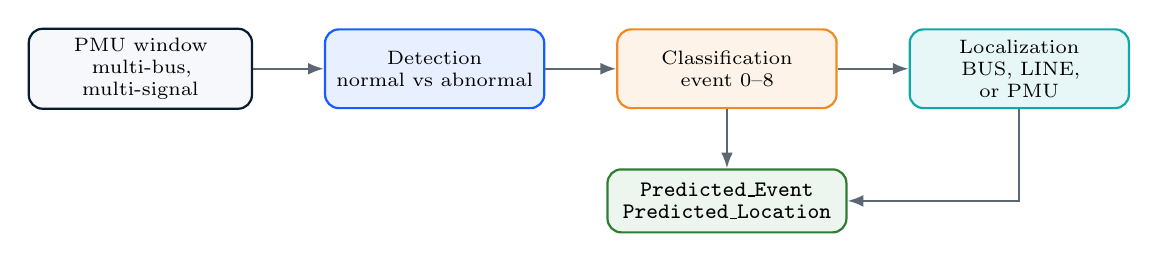
\begin{tikzpicture}[
  node distance=0.5cm and 0.9cm,
  raw/.style={rounded corners=5pt,draw=Navy,fill=Paper,thick,text width=2.6cm,minimum height=1cm,align=center,font=\scriptsize},
  taskblue/.style={rounded corners=5pt,draw=Blue,fill=Blue!10,thick,text width=2.55cm,minimum height=1cm,align=center,font=\scriptsize},
  taskorange/.style={rounded corners=5pt,draw=Orange,fill=Orange!10,thick,text width=2.55cm,minimum height=1cm,align=center,font=\scriptsize},
  taskcyan/.style={rounded corners=5pt,draw=Cyan,fill=Cyan!10,thick,text width=2.55cm,minimum height=1cm,align=center,font=\scriptsize},
  outbox/.style={rounded corners=5pt,draw=Green,fill=SoftGreen,thick,text width=2.8cm,minimum height=0.8cm,align=center,font=\scriptsize},
  arrow/.style={-{Latex[length=2mm]},thick,draw=Muted}
]
\node[raw] (pmu) {PMU window\\multi-bus, multi-signal};
\node[taskblue,right=of pmu] (det) {Detection\\normal vs abnormal};
\node[taskorange,right=of det] (cls) {Classification\\event 0--8};
\node[taskcyan,right=of cls] (loc) {Localization\\BUS, LINE, or PMU};
\node[outbox,below=0.75cm of cls] (csv) {\code{Predicted\_Event}\\\code{Predicted\_Location}};
\draw[arrow] (pmu) -- (det);
\draw[arrow] (det) -- (cls);
\draw[arrow] (cls) -- (loc);
\draw[arrow] (loc) |- (csv);
\draw[arrow] (cls) -- (csv);
\end{tikzpicture}
\vspace{3mm}
\begin{block}{Design consequence}
The pipeline keeps these decisions separate: a physical classifier, missing/bad-data detectors, and typed localizers replace one flat classifier.
\end{block}
\end{frame}

% -------------------------------------------------------------------
\begin{frame}{Event labels}
\small
\centering
\begin{tabular}{clp{0.55\textwidth}}
\toprule
\textbf{Label} & \textbf{Name} & \textbf{Physical interpretation}\\
\midrule
0 & normal & No physical disturbance and no major data issue.\\
1 & fault & Strong voltage disturbance, fast derivative, sag or transient.\\
2 & line outage & Current redistribution without fault-level voltage collapse.\\
3 & generation change & Frequency/ROCOF and active-power proxy change.\\
4 & load change & Sustained current and power-consumption change.\\
5 & missing data & Data loss without strong physical evidence.\\
6 & missing + physical & Data loss combined with a real physical event.\\
7 & bad data & One sensor/channel becomes inconsistent with the rest.\\
8 & unknown / mixed proxy & Official unknown class; implemented as mixed physical evidence not cleanly explained by 1--4.\\
\bottomrule
\end{tabular}
\end{frame}

% -------------------------------------------------------------------
\fi
\begin{frame}{PMU signals and phasor inputs}
\small
\begin{columns}[T,totalwidth=\textwidth]
\begin{column}{0.50\textwidth}
\begin{block}{Raw columns}
\scriptsize
\begin{tabular}{ll}
\toprule
Group & Columns\\
\midrule
Voltage magnitude & \code{VA\_MAG, VB\_MAG, VC\_MAG}\\
Current magnitude & \code{IA\_MAG, IB\_MAG, IC\_MAG}\\
Voltage angle & \code{VA\_ANG, VB\_ANG, VC\_ANG}\\
Current angle & \code{IA\_ANG, IB\_ANG, IC\_ANG}\\
Dynamics & \code{Freq, ROCOF}\\
Quality/time & \code{DATA\_PRESENT, TIMESTAMP}\\
\bottomrule
\end{tabular}
\end{block}
\begin{exampleblock}{Observed PMUs}
Buses 2, 5, 6, 10, 19, 22, 29, and 39.
\end{exampleblock}
\end{column}
\begin{column}{0.46\textwidth}
\begin{block}{Measurement model}
\[
V_{\phi}(t)=|V_{\phi}(t)|e^{j\theta^V_{\phi}(t)},\quad
I_{\phi}(t)=|I_{\phi}(t)|e^{j\theta^I_{\phi}(t)}
\]
\[
\phi\in\{A,B,C\},\qquad
\theta_{\mathrm{rad}}=\pi\theta_{\mathrm{deg}}/180
\]
\[
\dot f(t)=\mathrm{ROCOF}(t)
\]
\end{block}
\begin{alertblock}{Inference scope}
The extractor uses magnitudes, unwrapped angles, frequency, ROCOF, and availability. It does not solve a full AC power-flow at inference time.
\end{alertblock}
\end{column}
\end{columns}
\end{frame}

\iffalse
\begin{frame}{Raw PMU signals}
\small
\begin{columns}[T,totalwidth=\textwidth]
\begin{column}{0.49\textwidth}
\begin{block}{Electrical measurements}
\begin{tabular}{ll}
\toprule
Group & Columns\\
\midrule
Voltage magnitude & \code{VA\_MAG, VB\_MAG, VC\_MAG}\\
Current magnitude & \code{IA\_MAG, IB\_MAG, IC\_MAG}\\
Voltage angle & \code{VA\_ANG, VB\_ANG, VC\_ANG}\\
Current angle & \code{IA\_ANG, IB\_ANG, IC\_ANG}\\
Dynamics & \code{Freq, ROCOF}\\
\bottomrule
\end{tabular}
\end{block}
\end{column}
\begin{column}{0.47\textwidth}
\begin{block}{Support variables}
\begin{itemize}
  \item \code{TIMESTAMP}: time alignment.
  \item \code{DATA\_PRESENT}: measurement availability.
  \item Bus ID from \code{Bus*.csv}; official PMUs are buses 2, 5, 6, 10, 19, 22, 29, and 39.
  \item IEEE 39-bus topology for graph features.
\end{itemize}
\end{block}
\begin{exampleblock}{Interpretation}
Every feature family is built from a physical question: how large, how fast, how persistent, how coherent, and where in the grid?
\end{exampleblock}
\end{column}
\end{columns}
\end{frame}

% -------------------------------------------------------------------
\begin{frame}{PMU measurement model}
\small
\begin{columns}[T,totalwidth=\textwidth]
\begin{column}{0.50\textwidth}
\begin{block}{Per bus, per phase}
\[
V_{\phi}(t)=|V_{\phi}(t)|e^{j\theta^V_{\phi}(t)},\qquad
I_{\phi}(t)=|I_{\phi}(t)|e^{j\theta^I_{\phi}(t)}
\]
\[
\phi \in \{A,B,C\},\qquad
\theta_{\mathrm{rad}}=\frac{\pi}{180}\theta_{\mathrm{deg}}
\]
\[
\dot{f}(t)=\mathrm{ROCOF}(t)
\]
\end{block}
\begin{exampleblock}{Feature inputs}
The extractor uses magnitudes, unwrapped angles, frequency, ROCOF, and data availability. It does not solve a full AC power-flow at inference time.
\end{exampleblock}
\end{column}
\begin{column}{0.46\textwidth}
\centering
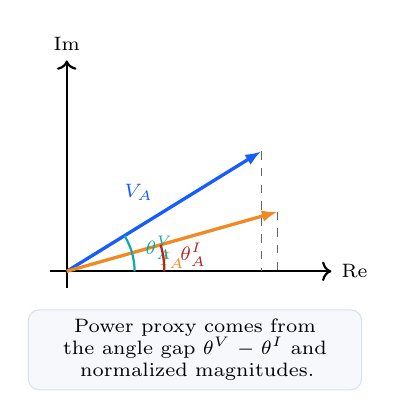
\begin{tikzpicture}[scale=1.05]
  \draw[->,thick] (-0.2,0) -- (3.2,0) node[right]{\scriptsize Re};
  \draw[->,thick] (0,-0.2) -- (0,2.55) node[above]{\scriptsize Im};
  \draw[Blue,very thick,-{Latex[length=2mm]}] (0,0) -- (2.35,1.45) node[midway,above left]{\scriptsize $V_A$};
  \draw[Orange,very thick,-{Latex[length=2mm]}] (0,0) -- (2.55,0.72) node[midway,below]{\scriptsize $I_A$};
  \draw[Cyan,thick] (0.82,0) arc[start angle=0,end angle=31.7,radius=0.82];
  \node[Cyan] at (1.12,0.28) {\scriptsize $\theta^V_A$};
  \draw[Red,thick] (1.18,0) arc[start angle=0,end angle=15.8,radius=1.18];
  \node[Red] at (1.53,0.20) {\scriptsize $\theta^I_A$};
  \draw[Muted,dashed] (2.35,1.45) -- (2.35,0);
  \draw[Muted,dashed] (2.55,0.72) -- (2.55,0);
  \node[rounded corners=4pt,draw=Line,fill=Paper,text width=4.0cm,align=center,font=\scriptsize] at (1.55,-0.95)
  {Power proxy comes from the angle gap $\theta^V-\theta^I$ and normalized magnitudes.};
\end{tikzpicture}
\end{column}
\end{columns}
\end{frame}

% -------------------------------------------------------------------
\fi
\begin{frame}{IEEE 39-bus system view}
\small
\begin{columns}[T,totalwidth=\textwidth]
\begin{column}{0.56\textwidth}
\centering
\resizebox{\linewidth}{!}{%
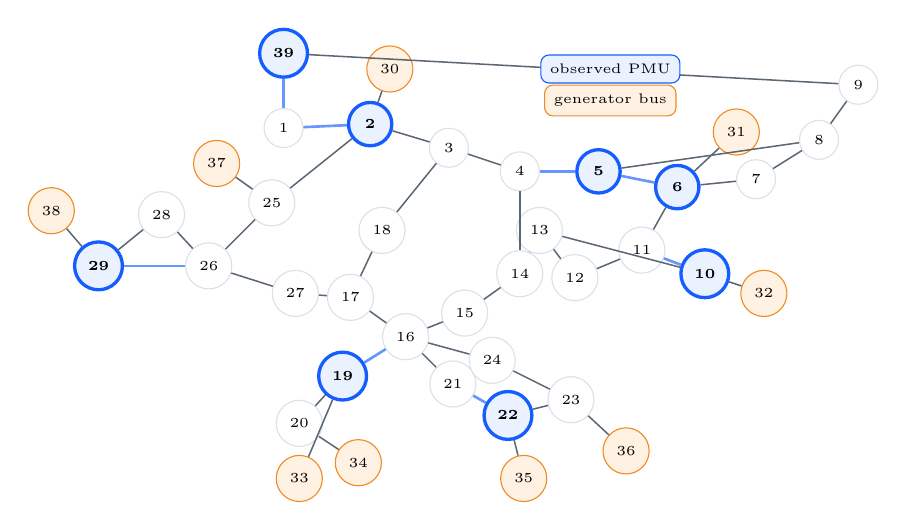
\begin{tikzpicture}[
  bus/.style={circle,draw=Line,fill=white,minimum size=0.44cm,font=\tiny},
  pmu/.style={circle,draw=Blue,fill=SoftBlue,very thick,minimum size=0.55cm,font=\tiny\bfseries},
  gen/.style={circle,draw=Orange,fill=SoftOrange,minimum size=0.46cm,font=\tiny},
  line/.style={draw=Muted,line width=0.55pt},
  obsline/.style={draw=Blue!65,line width=0.95pt}
]
\node[bus] (b1) at (0.0,2.1) {1};
\node[pmu] (b2) at (1.1,2.15) {2};
\node[bus] (b3) at (2.1,1.85) {3};
\node[bus] (b4) at (3.0,1.55) {4};
\node[pmu] (b5) at (4.0,1.55) {5};
\node[pmu] (b6) at (5.0,1.35) {6};
\node[bus] (b7) at (6.0,1.45) {7};
\node[bus] (b8) at (6.8,1.95) {8};
\node[bus] (b9) at (7.3,2.65) {9};
\node[pmu] (b39) at (0.0,3.05) {39};
\node[pmu] (b10) at (5.35,0.25) {10};
\node[bus] (b11) at (4.55,0.55) {11};
\node[bus] (b12) at (3.70,0.20) {12};
\node[bus] (b13) at (3.25,0.80) {13};
\node[bus] (b14) at (3.00,0.25) {14};
\node[bus] (b15) at (2.30,-0.25) {15};
\node[bus] (b16) at (1.55,-0.55) {16};
\node[bus] (b17) at (0.85,-0.05) {17};
\node[bus] (b18) at (1.25,0.80) {18};
\node[pmu] (b19) at (0.75,-1.05) {19};
\node[bus] (b20) at (0.2,-1.65) {20};
\node[bus] (b21) at (2.15,-1.15) {21};
\node[pmu] (b22) at (2.85,-1.55) {22};
\node[bus] (b23) at (3.65,-1.35) {23};
\node[bus] (b24) at (2.65,-0.85) {24};
\node[bus] (b25) at (-0.15,1.15) {25};
\node[bus] (b26) at (-0.95,0.35) {26};
\node[bus] (b27) at (0.15,0.00) {27};
\node[bus] (b28) at (-1.55,1.00) {28};
\node[pmu] (b29) at (-2.35,0.35) {29};
\node[gen] (b30) at (1.35,2.85) {30};
\node[gen] (b31) at (5.75,2.05) {31};
\node[gen] (b32) at (6.10,0.00) {32};
\node[gen] (b33) at (0.20,-2.35) {33};
\node[gen] (b34) at (0.95,-2.15) {34};
\node[gen] (b35) at (3.05,-2.35) {35};
\node[gen] (b36) at (4.35,-2.00) {36};
\node[gen] (b37) at (-0.85,1.65) {37};
\node[gen] (b38) at (-2.95,1.05) {38};
\foreach \a/\b in {b1/b2,b1/b39,b2/b3,b2/b25,b2/b30,b3/b4,b3/b18,b4/b5,b4/b14,b5/b6,b5/b8,b6/b7,b6/b11,b6/b31,b7/b8,b8/b9,b9/b39,b10/b11,b10/b13,b10/b32,b11/b12,b12/b13,b13/b14,b14/b15,b15/b16,b16/b17,b16/b19,b16/b21,b16/b24,b17/b18,b17/b27,b19/b20,b19/b33,b20/b34,b21/b22,b22/b23,b22/b35,b23/b24,b23/b36,b25/b26,b25/b37,b26/b27,b26/b28,b26/b29,b28/b29,b29/b38} {
  \draw[line] (\a) -- (\b);
}
\foreach \a/\b in {b1/b2,b4/b5,b5/b6,b16/b19,b21/b22,b26/b29,b1/b39,b10/b11} {
  \draw[obsline] (\a) -- (\b);
}
\node[rounded corners=3pt,draw=Blue,fill=SoftBlue,font=\tiny] at (4.15,2.85) {observed PMU};
\node[rounded corners=3pt,draw=Orange,fill=SoftOrange,font=\tiny] at (4.15,2.45) {generator bus};
\end{tikzpicture}
}
\end{column}
\begin{column}{0.40\textwidth}
\scriptsize
\begin{block}{Observed PMUs}
\centering $\{2,5,6,10,19,22,29,39\}$
\end{block}
\begin{exampleblock}{Electrical reading}
The localizer sees eight sparse PMU views. Events must be inferred from the disturbance pattern across those locations.
\end{exampleblock}
\begin{alertblock}{Topology used}
Electrical distances come from the IEEE 39-bus admittance model, not drawing geometry.
\end{alertblock}
\end{column}
\end{columns}
\end{frame}

% -------------------------------------------------------------------
\begin{frame}{Topology math: from branches to electrical distance}
\small
\begin{columns}[T,totalwidth=\textwidth]
\begin{column}{0.49\textwidth}
\begin{block}{Admittance and impedance}
\[
Y_{\mathrm{bus}}:\ \text{network admittance matrix}
\]
\[
Z_{\mathrm{bus}}=Y_{\mathrm{bus}}^{+}
\]
\[
d_{ij}^{\mathrm{eff}}=
\left|Z_{ii}+Z_{jj}-Z_{ij}-Z_{ji}\right|
\]
\end{block}
\begin{exampleblock}{Meaning}
Two buses are close if an injection at one bus is expected to have a similar voltage effect at the other.
\end{exampleblock}
\end{column}
\begin{column}{0.47\textwidth}
\centering
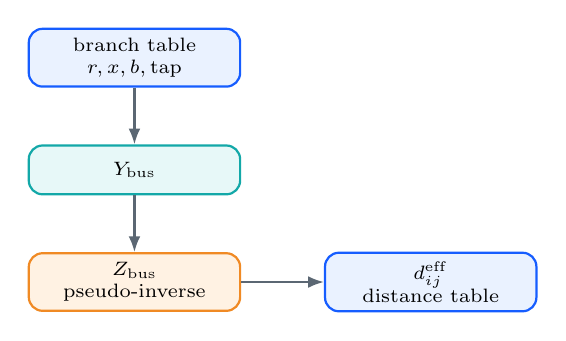
\begin{tikzpicture}[
  node distance=0.72cm,
  box/.style={rounded corners=5pt,draw=Blue,fill=SoftBlue,thick,text width=2.45cm,minimum height=0.62cm,align=center,font=\scriptsize},
  box2/.style={rounded corners=5pt,draw=Cyan,fill=SoftCyan,thick,text width=2.45cm,minimum height=0.62cm,align=center,font=\scriptsize},
  box3/.style={rounded corners=5pt,draw=Orange,fill=SoftOrange,thick,text width=2.45cm,minimum height=0.62cm,align=center,font=\scriptsize},
  arrow/.style={-{Latex[length=2mm]},thick,draw=Muted}
]
\node[box] (br) {branch table\\$r,x,b,\mathrm{tap}$};
\node[box2,below=of br] (y) {$Y_{\mathrm{bus}}$};
\node[box3,below=of y] (z) {$Z_{\mathrm{bus}}$\\pseudo-inverse};
\node[box,right=1.05cm of z] (dist) {$d_{ij}^{\mathrm{eff}}$\\distance table};
\draw[arrow] (br) -- (y);
\draw[arrow] (y) -- (z);
\draw[arrow] (z) -- (dist);
\end{tikzpicture}
\vspace{0mm}
\begin{alertblock}{Where it appears}
Graph-temporal features use $1/d_{ij}^{\mathrm{eff}}$ weights.
\end{alertblock}
\end{column}
\end{columns}
\end{frame}

% -------------------------------------------------------------------
\begin{frame}{Case representation before feature extraction}
\small
\begin{columns}[T,totalwidth=\textwidth]
\begin{column}{0.56\textwidth}
\centering
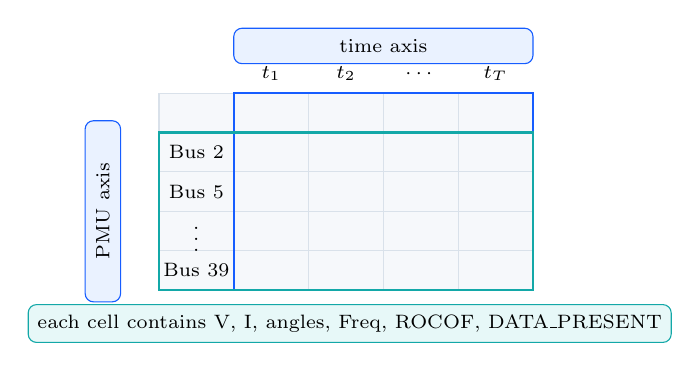
\begin{tikzpicture}[x=0.95cm,y=0.50cm]
  \foreach \r in {0,...,4} {
    \foreach \c in {0,...,4} {
      \draw[Line,fill=Paper] (\c,-\r) rectangle +(1,-1);
    }
  }
  \node[font=\scriptsize] at (1.5,0.5) {$t_1$};
  \node[font=\scriptsize] at (2.5,0.5) {$t_2$};
  \node[font=\scriptsize] at (3.5,0.5) {$\cdots$};
  \node[font=\scriptsize] at (4.5,0.5) {$t_T$};
  \node[font=\scriptsize] at (0.5,-1.5) {Bus 2};
  \node[font=\scriptsize] at (0.5,-2.5) {Bus 5};
  \node[font=\scriptsize] at (0.5,-3.5) {$\vdots$};
  \node[font=\scriptsize] at (0.5,-4.5) {Bus 39};
  \draw[Blue,thick] (1,0) rectangle (5,-5);
  \draw[Cyan,thick] (0,-1) rectangle (5,-5);
  \node[rounded corners=3pt,draw=Blue,fill=SoftBlue,font=\scriptsize,minimum width=3.8cm,minimum height=0.45cm] at (3,1.2) {time axis};
  \node[rounded corners=3pt,draw=Blue,fill=SoftBlue,font=\scriptsize,rotate=90,minimum width=2.3cm,minimum height=0.45cm] at (-0.75,-3) {PMU axis};
  \node[rounded corners=3pt,draw=Cyan,fill=SoftCyan,font=\scriptsize,minimum width=5.3cm,minimum height=0.48cm] at (2.55,-5.85) {each cell contains V, I, angles, Freq, ROCOF, DATA\_PRESENT};
\end{tikzpicture}
\end{column}
\begin{column}{0.40\textwidth}
\begin{block}{The extractor reads a tensor}
One case is a PMU-by-time table. Each cell contains voltage, current, angle, frequency, ROCOF, and availability channels.
\end{block}
\begin{alertblock}{Extracted representation}
The window becomes one row of engineered features. Models never see the raw tensor directly.
\end{alertblock}
\end{column}
\end{columns}
\end{frame}

% -------------------------------------------------------------------

% -------------------------------------------------------------------
\begin{frame}{Runtime route and end-to-end method}
\small
\begin{columns}[T,totalwidth=\textwidth]
\begin{column}{0.43\textwidth}
\begin{block}{Entrypoint}
\code{python main.py --input-dir <folder> --output <csv>}
\end{block}
\begin{exampleblock}{Active route}
\code{sgms\_extra\_trees\_windowed}, \code{ml\_windowed}, 30 s windows.
\end{exampleblock}
\begin{alertblock}{Fallback}
The bus-agnostic physics runtime is only a missing-bundle fallback.
\end{alertblock}
\end{column}
\begin{column}{0.53\textwidth}
\centering
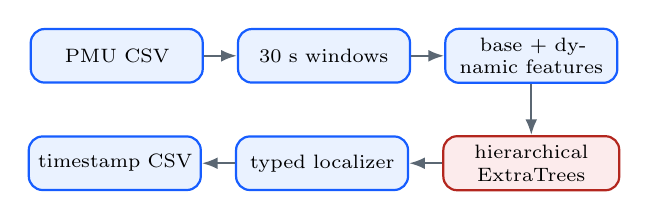
\begin{tikzpicture}[
  node distance=0.42cm,
  box/.style={rounded corners=5pt,draw=Blue,fill=SoftBlue,thick,text width=1.95cm,minimum height=0.68cm,align=center,font=\scriptsize},
  model/.style={rounded corners=5pt,draw=Red,fill=SoftRed,thick,text width=2.0cm,minimum height=0.68cm,align=center,font=\scriptsize},
  arrow/.style={-{Latex[length=2mm]},thick,draw=Muted}
]
\node[box] (raw) {PMU CSV};
\node[box,right=of raw] (win) {30 s windows};
\node[box,right=of win] (feat) {base + dynamic features};
\node[model,below=0.65cm of feat] (clf) {hierarchical ExtraTrees};
\node[box,left=of clf] (loc) {typed localizer};
\node[box,left=of loc] (out) {timestamp CSV};
\draw[arrow] (raw) -- (win);
\draw[arrow] (win) -- (feat);
\draw[arrow] (feat) -- (clf);
\draw[arrow] (clf) -- (loc);
\draw[arrow] (loc) -- (out);
\end{tikzpicture}
\vspace{1mm}
\begin{block}{Runtime shape}
Each window becomes one physics-aware feature row. The output is expanded back to timestamp-bus rows for the official CSV.
\end{block}
\end{column}
\end{columns}
\end{frame}

\iffalse
\begin{frame}{Final runtime route}
\small
\begin{columns}[T,totalwidth=\textwidth]
\begin{column}{0.47\textwidth}
\begin{block}{Entrypoint}
\code{python main.py --input-dir <folder> --output <csv>}
\end{block}
\begin{block}{Active route}
\begin{itemize}
  \item \code{model = sgms\_extra\_trees\_windowed}
  \item \code{route = ml\_windowed}
  \item \code{window\_seconds = 30}
\end{itemize}
\end{block}
\end{column}
\begin{column}{0.49\textwidth}
\begin{exampleblock}{Call chain}
\code{main.py}\\
$\rightarrow$ \code{src/models/hybrid\_submission.py}\\
$\rightarrow$ \code{src/data\_factory/final\_model.py}
\end{exampleblock}
\begin{alertblock}{Fallback}
A bus-agnostic physics runtime remains only as a missing-bundle fallback.
\end{alertblock}
\end{column}
\end{columns}
\end{frame}

% -------------------------------------------------------------------
\begin{frame}{End-to-end method}
\centering
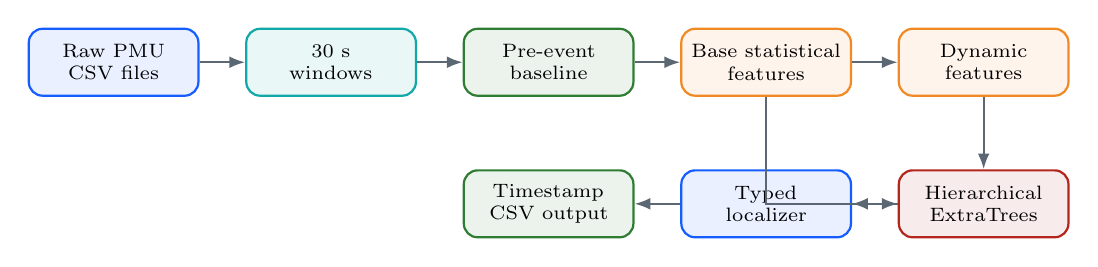
\begin{tikzpicture}[
  node distance=0.58cm,
  boxblue/.style={rounded corners=5pt,draw=Blue,fill=Blue!9,thick,text width=1.92cm,minimum height=0.85cm,align=center,font=\scriptsize},
  boxcyan/.style={rounded corners=5pt,draw=Cyan,fill=Cyan!9,thick,text width=1.92cm,minimum height=0.85cm,align=center,font=\scriptsize},
  boxgreen/.style={rounded corners=5pt,draw=Green,fill=Green!9,thick,text width=1.92cm,minimum height=0.85cm,align=center,font=\scriptsize},
  boxorange/.style={rounded corners=5pt,draw=Orange,fill=Orange!9,thick,text width=1.92cm,minimum height=0.85cm,align=center,font=\scriptsize},
  boxred/.style={rounded corners=5pt,draw=Red,fill=Red!9,thick,text width=1.92cm,minimum height=0.85cm,align=center,font=\scriptsize},
  arrow/.style={-{Latex[length=2mm]},thick,draw=Muted}
]
\node[boxblue] (raw) {Raw PMU\\CSV files};
\node[boxcyan,right=of raw] (win) {30 s\\windows};
\node[boxgreen,right=of win] (base) {Pre-event\\baseline};
\node[boxorange,right=of base] (feat) {Base statistical\\features};
\node[boxorange,right=of feat] (dyn) {Dynamic\\features};
\node[boxred,below=0.92cm of dyn] (clf) {Hierarchical\\ExtraTrees};
\node[boxblue,left=of clf] (loc) {Typed\\localizer};
\node[boxgreen,left=of loc] (csv) {Timestamp\\CSV output};
\draw[arrow] (raw) -- (win);
\draw[arrow] (win) -- (base);
\draw[arrow] (base) -- (feat);
\draw[arrow] (feat) -- (dyn);
\draw[arrow] (dyn) -- (clf);
\draw[arrow] (feat) |- (clf);
\draw[arrow] (clf) -- (loc);
\draw[arrow] (loc) -- (csv);
\end{tikzpicture}
\vspace{3mm}
\begin{block}{Runtime shape}
We convert each PMU window into a physics-aware signature, classify the event with guarded ExtraTrees models, then localize it with event-specific localizers.
\end{block}
\end{frame}

% -------------------------------------------------------------------
\fi
\begin{frame}{Window predictions to timestamp rows}
\small
\centering
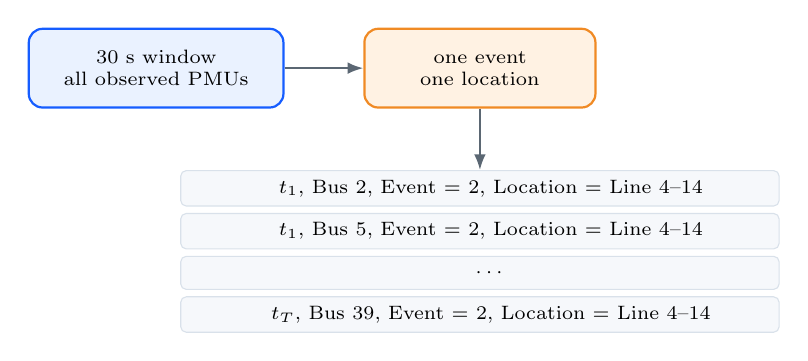
\begin{tikzpicture}[
  node distance=0.7cm,
  win/.style={rounded corners=5pt,draw=Blue,fill=SoftBlue,thick,text width=3.0cm,minimum height=1.0cm,align=center,font=\scriptsize},
  pred/.style={rounded corners=5pt,draw=Orange,fill=SoftOrange,thick,text width=2.7cm,minimum height=1.0cm,align=center,font=\scriptsize},
  row/.style={rounded corners=2pt,draw=Line,fill=Paper,minimum width=7.6cm,minimum height=0.42cm,align=left,font=\scriptsize},
  arrow/.style={-{Latex[length=2mm]},thick,draw=Muted}
]
\node[win] (w) {30 s window\\all observed PMUs};
\node[pred,right=1.0cm of w] (p) {one event\\one location};
\node[row,below=0.78cm of p] (r1) {\quad $t_1$, Bus 2, Event = 2, Location = Line 4--14};
\node[row,below=0.08cm of r1] (r2) {\quad $t_1$, Bus 5, Event = 2, Location = Line 4--14};
\node[row,below=0.08cm of r2] (r3) {\quad $\cdots$};
\node[row,below=0.08cm of r3] (r4) {\quad $t_T$, Bus 39, Event = 2, Location = Line 4--14};
\draw[arrow] (w) -- (p);
\draw[arrow] (p) -- (r1);
\end{tikzpicture}
\vspace{2mm}
\begin{block}{Submission contract}
The official CSV is timestamp-aligned even though the decision is made at the window level.
\end{block}
\end{frame}

% -------------------------------------------------------------------
\section{Windowing and Baseline}
\sectionframe{}{Windowing and Baseline}{30-second windows and segment statistics}


% -------------------------------------------------------------------
\begin{frame}{30-second window and segment design}
\small
\begin{columns}[T,totalwidth=\textwidth]
\begin{column}{0.58\textwidth}
\centering
\resizebox{\linewidth}{!}{%
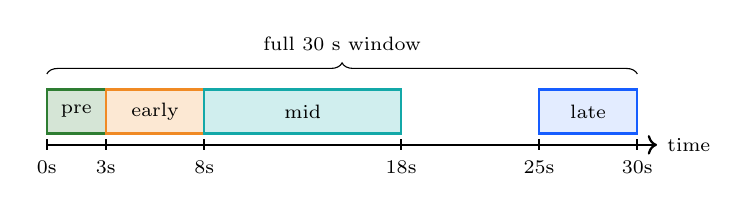
\begin{tikzpicture}[x=0.25cm,y=0.9cm]
  \draw[->,thick] (0,0) -- (31,0) node[right]{\scriptsize time};
  \foreach \x/\txt in {0/0s,3/3s,8/8s,18/18s,25/25s,30/30s} {
    \draw[thick] (\x,0.08) -- (\x,-0.08) node[below]{\scriptsize \txt};
  }
  \fill[Green!20] (0,0.16) rectangle (3,0.78);
  \fill[Orange!20] (3,0.16) rectangle (8,0.78);
  \fill[Cyan!20] (8,0.16) rectangle (18,0.78);
  \fill[Blue!12] (25,0.16) rectangle (30,0.78);
  \draw[Green,thick] (0,0.16) rectangle (3,0.78);
  \draw[Orange,thick] (3,0.16) rectangle (8,0.78);
  \draw[Cyan,thick] (8,0.16) rectangle (18,0.78);
  \draw[Blue,thick] (25,0.16) rectangle (30,0.78);
  \node at (1.5,0.47) {\scriptsize pre};
  \node at (5.5,0.47) {\scriptsize early};
  \node at (13,0.47) {\scriptsize mid};
  \node at (27.5,0.47) {\scriptsize late};
  \draw[decorate,decoration={brace,amplitude=4pt}] (0,1.0) -- node[above=5pt]{\scriptsize full 30 s window} (30,1.0);
\end{tikzpicture}}
\end{column}
\begin{column}{0.38\textwidth}
\begin{block}{Segments}
\[
S_{\mathrm{pre}}=[0,3),\quad S_{\mathrm{early}}=[3,8)
\]
\[
S_{\mathrm{mid}}=[8,18),\quad S_{\mathrm{late}}=[25,30)
\]
\[
S_{\mathrm{full}}=[0,30)
\]
\end{block}
\begin{alertblock}{Reason}
The window is long enough to capture onset, transient, and settling, but short enough to produce one stable event decision.
\end{alertblock}
\end{column}
\end{columns}
\end{frame}

\iffalse
\begin{frame}{30-second window design}
\small
\begin{columns}[T,totalwidth=\textwidth]
\begin{column}{0.55\textwidth}
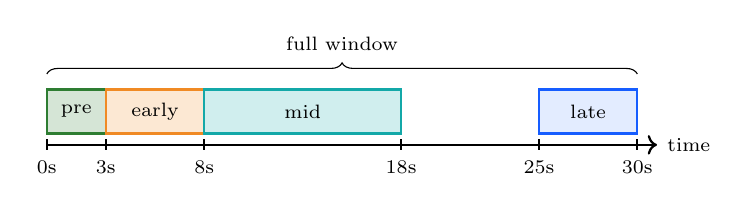
\begin{tikzpicture}[x=0.25cm,y=0.9cm]
  \draw[->,thick] (0,0) -- (31,0) node[right]{\scriptsize time};
  \foreach \x/\txt in {0/0s,3/3s,8/8s,18/18s,25/25s,30/30s} {
    \draw[thick] (\x,0.08) -- (\x,-0.08) node[below]{\scriptsize \txt};
  }
  \fill[Green!20] (0,0.16) rectangle (3,0.78);
  \fill[Orange!20] (3,0.16) rectangle (8,0.78);
  \fill[Cyan!20] (8,0.16) rectangle (18,0.78);
  \fill[Blue!12] (25,0.16) rectangle (30,0.78);
  \draw[Green,thick] (0,0.16) rectangle (3,0.78);
  \draw[Orange,thick] (3,0.16) rectangle (8,0.78);
  \draw[Cyan,thick] (8,0.16) rectangle (18,0.78);
  \draw[Blue,thick] (25,0.16) rectangle (30,0.78);
  \node at (1.5,0.47) {\scriptsize pre};
  \node at (5.5,0.47) {\scriptsize early};
  \node at (13,0.47) {\scriptsize mid};
  \node at (27.5,0.47) {\scriptsize late};
  \draw[decorate,decoration={brace,amplitude=4pt}] (0,1.0) -- node[above=5pt]{\scriptsize full window} (30,1.0);
\end{tikzpicture}
\end{column}
\begin{column}{0.41\textwidth}
\begin{block}{Window evidence}
\begin{itemize}
  \item One sample is too noisy.
  \item A fault has onset and transient.
  \item Load/generation changes are often slower.
  \item Missing data needs run-length evidence.
\end{itemize}
\end{block}
\end{column}
\end{columns}
\vspace{1mm}
\begin{exampleblock}{Runtime behavior}
The model predicts once per window and replicates the window prediction to all required timestamp/bus rows.
\end{exampleblock}
\end{frame}

% -------------------------------------------------------------------

% -------------------------------------------------------------------
\begin{frame}{Window segmentation math}
\small
\begin{columns}[T,totalwidth=\textwidth]
\begin{column}{0.52\textwidth}
\begin{block}{Given one 30-second window}
\[
t_0=\min(t),\qquad t_1=\max(t),\qquad t_p=t_0+3
\]
\[
\mathcal{T}_{pre}=\{t:t\le t_p\}
\]
\[
\mathcal{T}_{early}=\{t:t_p<t\le t_p+5\}
\]
\[
\mathcal{T}_{mid}=\{t:t_p+5<t\le t_p+15\}
\]
\[
\mathcal{T}_{late}=\{t:t\ge \max(t_p,t_1-5)\}
\]
\end{block}
\end{column}
\begin{column}{0.44\textwidth}
\centering
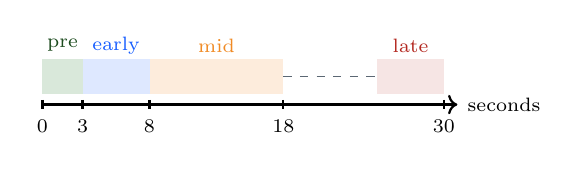
\begin{tikzpicture}[x=0.17cm,y=0.75cm]
  \draw[->,thick] (0,0) -- (31,0) node[right]{\scriptsize seconds};
  \foreach \x/\lab in {0/0,3/3,8/8,18/18,30/30} {
    \draw[thick] (\x,0.08) -- (\x,-0.08) node[below]{\scriptsize \lab};
  }
  \fill[Green!18] (0,0.18) rectangle (3,0.78);
  \fill[Blue!14] (3,0.18) rectangle (8,0.78);
  \fill[Orange!16] (8,0.18) rectangle (18,0.78);
  \fill[Red!12] (25,0.18) rectangle (30,0.78);
  \node[Green!60!black] at (1.5,1.0) {\scriptsize pre};
  \node[Blue] at (5.5,1.0) {\scriptsize early};
  \node[Orange] at (13,1.0) {\scriptsize mid};
  \node[Red] at (27.5,1.0) {\scriptsize late};
  \draw[Muted,dashed] (18,0.48) -- (25,0.48);
\end{tikzpicture}
\vspace{3mm}
\begin{exampleblock}{Temporal alignment}
Event labels are window labels, but electrical signatures are time-shaped. These masks let us compare the same signal before and after the disturbance.
\end{exampleblock}
\end{column}
\end{columns}
\end{frame}

% -------------------------------------------------------------------

% -------------------------------------------------------------------
\fi
\begin{frame}{Local baseline, robust scale, and subtraction}
\small
\begin{columns}[T,totalwidth=\textwidth]
\begin{column}{0.45\textwidth}
\begin{block}{Per PMU and signal}
\[
b_{p,s}=\mathrm{median}_{t\in S_{\mathrm{pre}}}x_{p,s}(t)
\]
\[
\sigma_{p,s}^{\mathrm{rob}}=1.4826\,\mathrm{median}_{t\in S_{\mathrm{pre}}}|x_{p,s}(t)-b_{p,s}|+\epsilon
\]
\[
x'_{p,s}(t)=x_{p,s}(t)-b_{p,s}
\]
\[
z_{p,s}(t)=|x'_{p,s}(t)|/\sigma_{p,s}^{\mathrm{rob}}
\]
\end{block}
\end{column}
\begin{column}{0.51\textwidth}
\centering
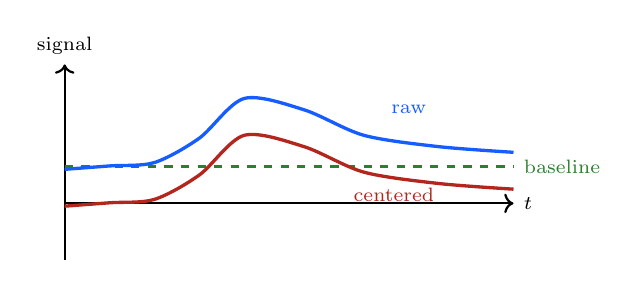
\begin{tikzpicture}[x=0.19cm,y=0.72cm]
  \draw[->,thick] (0,0) -- (30,0) node[right]{\scriptsize $t$};
  \draw[->,thick] (0,-1.0) -- (0,2.45) node[above]{\scriptsize signal};
  \draw[Green,thick,dashed] (0,0.65) -- (30,0.65) node[right]{\scriptsize baseline};
  \draw[Blue,very thick] plot[smooth] coordinates {(0,0.60) (3,0.66) (6,0.72) (9,1.15) (12,1.85) (16,1.65) (20,1.20) (25,1.00) (30,0.90)};
  \draw[Red,very thick] plot[smooth] coordinates {(0,-0.05) (3,0.01) (6,0.07) (9,0.50) (12,1.20) (16,1.00) (20,0.55) (25,0.35) (30,0.25)};
  \node[Blue] at (23,1.65) {\scriptsize raw};
  \node[Red] at (22,0.15) {\scriptsize centered};
\end{tikzpicture}
\begin{alertblock}{Scale fallback}
If MAD is too small, the code falls back to standard deviation and then to a safe value.
\end{alertblock}
\end{column}
\end{columns}
\end{frame}

\iffalse
\begin{frame}{Baseline and robust scale are computed locally}
\small
\begin{columns}[T,totalwidth=\textwidth]
\begin{column}{0.50\textwidth}
\begin{block}{For each bus $b$ and signal $s$}
\[
m_{b,s}=\mathrm{median}_{t\in \mathcal{T}_{pre}} x_{b,s}(t)
\]
\[
\tilde{x}_{b,s}(t)=x_{b,s}(t)-m_{b,s}
\]
\[
\sigma^{rob}_{b,s}=1.4826\cdot
\mathrm{median}_{t\in \mathcal{T}_{pre}}
\left|x_{b,s}(t)-m_{b,s}\right|
\]
\[
z_{b,s}(t)=
\frac{|x_{b,s}(t)-m_{b,s}|}{\max(\sigma^{rob}_{b,s},\epsilon)}
\]
\end{block}
\end{column}
\begin{column}{0.46\textwidth}
\centering
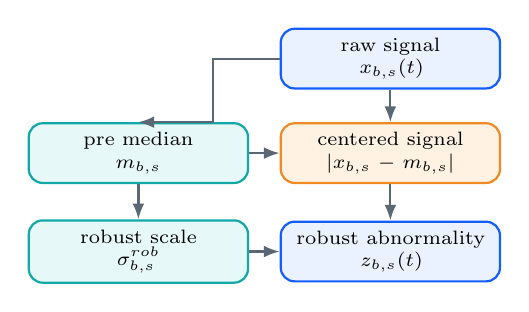
\begin{tikzpicture}[
  box/.style={rounded corners=5pt,draw=Blue,fill=SoftBlue,thick,text width=2.55cm,minimum height=0.72cm,align=center,font=\scriptsize},
  box2/.style={rounded corners=5pt,draw=Cyan,fill=SoftCyan,thick,text width=2.55cm,minimum height=0.72cm,align=center,font=\scriptsize},
  box3/.style={rounded corners=5pt,draw=Orange,fill=SoftOrange,thick,text width=2.55cm,minimum height=0.72cm,align=center,font=\scriptsize},
  arrow/.style={-{Latex[length=2mm]},thick,draw=Muted}
]
\node[box] (raw) at (3.2,1.55) {raw signal\\$x_{b,s}(t)$};
\node[box2] (med) at (0,0.35) {pre median\\$m_{b,s}$};
\node[box2] (scale) at (0,-0.90) {robust scale\\$\sigma^{rob}_{b,s}$};
\node[box3] (center) at (3.2,0.35) {centered signal\\$|x_{b,s}-m_{b,s}|$};
\node[box] (z) at (3.2,-0.90) {robust abnormality\\$z_{b,s}(t)$};
\draw[arrow] (raw.south) -- (center.north);
\draw[arrow] (raw.west) -- ++(-0.85,0) |- (med.north);
\draw[arrow] (med.east) -- (center.west);
\draw[arrow] (med.south) -- (scale.north);
\draw[arrow] (center.south) -- (z.north);
\draw[arrow] (scale.east) -- (z.west);
\end{tikzpicture}
\vspace{2mm}
\begin{alertblock}{Implementation detail}
If the MAD is too small, the code falls back to a standard deviation scale. If that also fails, it uses a safe fallback value.
\end{alertblock}
\end{column}
\end{columns}
\end{frame}

% -------------------------------------------------------------------
\begin{frame}{Baseline subtraction, visually}
\small
\begin{columns}[T,totalwidth=\textwidth]
\begin{column}{0.60\textwidth}
\centering
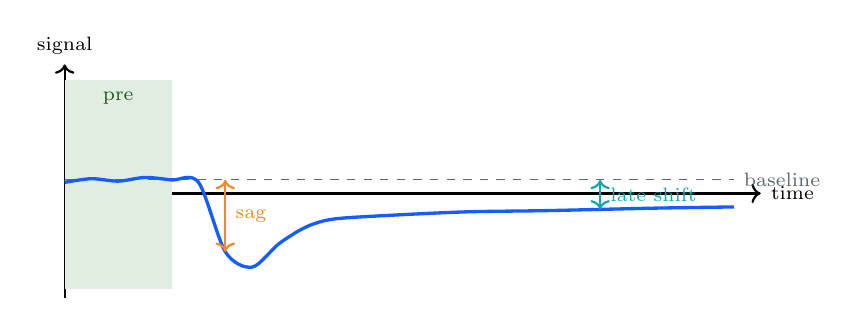
\begin{tikzpicture}[x=0.34cm,y=0.78cm]
  \draw[->,thick] (0,0) -- (26,0) node[right]{\scriptsize time};
  \draw[->,thick] (0,-1.7) -- (0,2.1) node[above]{\scriptsize signal};
  \fill[Green!14] (0,-1.55) rectangle (4,1.85);
  \node[Green!70!black] at (2,1.55) {\scriptsize pre};
  \draw[Muted,dashed] (0,0.22) -- (25,0.22) node[right]{\scriptsize baseline};
  \draw[Blue,very thick,smooth] plot coordinates {
    (0,0.18) (1,0.24) (2,0.20) (3,0.26) (4,0.22)
    (5,0.18) (6,-0.95) (7,-1.20) (8,-0.82) (9,-0.55)
    (10,-0.42) (12,-0.36) (15,-0.30) (18,-0.28) (22,-0.24) (25,-0.22)
  };
  \draw[Orange,<->,thick] (6,0.22) -- (6,-0.95) node[midway,right]{\scriptsize sag};
  \draw[Cyan,<->,thick] (20,0.22) -- (20,-0.26) node[midway,right]{\scriptsize late shift};
\end{tikzpicture}
\end{column}
\begin{column}{0.36\textwidth}
\begin{block}{Model input}
The feature extractor does not keep this curve. It records quantities such as early span, derivative, maximum deviation, and late shift.
\end{block}
\begin{exampleblock}{Fault reading}
A sharp voltage sag after the pre segment creates large derivative and large robust z-score features.
\end{exampleblock}
\end{column}
\end{columns}
\end{frame}

% -------------------------------------------------------------------
\fi
\section{Base Feature Engineering}
\sectionframe{}{Base Feature\\Engineering}{Per-window statistical feature families}

% -------------------------------------------------------------------
\begin{frame}{Feature schema and base families}
\scriptsize
\begin{columns}[T,totalwidth=\textwidth]
\begin{column}{0.47\textwidth}
\begin{block}{Canonical feature key}
\[
\texttt{<PMU/BUS>\_\_<SIGNAL>\_\_<SEGMENT>\_\_<STAT>}
\]
\code{Bus2\_\_VA\_MAG\_\_early\_\_span}\\
\code{Bus10\_\_Freq\_\_late\_\_mean}\\
\code{GLOBAL\_\_single\_signal\_score\_max}
\end{block}
\begin{alertblock}{Meaning}
The name stores source, physical signal, temporal segment, and statistic.
\end{alertblock}
\end{column}
\begin{column}{0.49\textwidth}
\centering
\begin{tabular}{p{0.38\linewidth}p{0.50\linewidth}}
\toprule
\textbf{Family} & \textbf{Purpose}\\
\midrule
Segment statistics & magnitude, spread, persistence\\
Temporal deltas & onset and post-event shift\\
Derivatives & fast transients and ramps\\
Robust z-score & scale-normalized abnormality\\
Sustained anomaly & duration above threshold\\
Data quality & NaNs, gaps, missing runs\\
Bad-data score & isolated channel faults\\
Phase spread & three-phase coherence\\
Power proxy & rough P/Q movement\\
Global aggregation & system-wide maxima and counts\\
\bottomrule
\end{tabular}
\end{column}
\end{columns}
\end{frame}

% -------------------------------------------------------------------
\begin{frame}{Feature grid and segment statistics}
\small
\begin{columns}[T,totalwidth=\textwidth]
\begin{column}{0.45\textwidth}
\begin{block}{Grid}
\[
N_{\mathrm{features}}\approx
N_{\mathrm{signals}}N_{\mathrm{segments}}N_{\mathrm{stats}}
\]
\[
+\ \text{cross and global terms}
\]
\end{block}
\begin{exampleblock}{Signals}
\code{VA\_MAG}, \code{IA\_MAG}, \code{VA\_ANG}, \code{IA\_ANG}, \code{Freq}, \code{ROCOF}, and related phase/channel variants.
\end{exampleblock}
\end{column}
\begin{column}{0.51\textwidth}
\begin{block}{Statistics per segment}
\[
\mu,\ \sigma,\ \min,\ \max,\ \mathrm{span},\ \mathrm{median}
\]
\[
\mathrm{MAD},\ p_{05},\ p_{95},\ |x|_{\max}
\]
\end{block}
\begin{alertblock}{Physical reading}
Statistics turn a curve into onset size, late offset, variability, and outlier amplitude.
\end{alertblock}
\end{column}
\end{columns}
\end{frame}

\iffalse
\begin{frame}{Feature naming convention}
\small
\begin{block}{Canonical pattern}
\[
\texttt{<PMU/BUS>\_\_<SIGNAL>\_\_<SEGMENT>\_\_<STATISTIC>}
\]
\end{block}
\begin{columns}[T,totalwidth=\textwidth]
\begin{column}{0.49\textwidth}
\begin{exampleblock}{Examples}
\code{Bus2\_\_VA\_MAG\_\_early\_\_span}\\
\code{Bus10\_\_Freq\_\_late\_\_mean}\\
\code{GLOBAL\_\_single\_signal\_score\_max}
\end{exampleblock}
\end{column}
\begin{column}{0.47\textwidth}
\begin{alertblock}{Reimplementation note}
The feature vector has tens of thousands of columns. A consistent naming scheme makes debugging and reimplementation possible.
\end{alertblock}
\end{column}
\end{columns}
\end{frame}

% -------------------------------------------------------------------
\section{Base Feature Engineering}
\sectionframe{}{Base Feature\\Engineering}{Per-window statistical feature families}


% -------------------------------------------------------------------
\begin{frame}{Base feature families}
\small
\centering
\begin{tabular}{p{0.23\textwidth}p{0.34\textwidth}p{0.32\textwidth}}
\toprule
\textbf{Family} & \textbf{Computed from} & \textbf{Physical signal}\\
\midrule
Segment statistics & every signal and segment & response magnitude and variability\\
Temporal deltas & early/mid/late vs pre & operating-point movement\\
Derivatives & finite differences & event abruptness\\
Robust z-score & pre-event median/MAD & abnormal signal magnitude\\
Data quality & gaps, NaNs, data-present & measurement availability\\
Single-signal anomaly & ranked abnormal channels & isolated channel corruption\\
Power proxy & V/I magnitudes and angles & active/reactive proxy movement\\
Global aggregations & PMU-level feature summaries & system-wide spatial pattern\\
\bottomrule
\end{tabular}
\end{frame}

% -------------------------------------------------------------------
\begin{frame}{Feature grid: signal $\times$ segment $\times$ statistic}
\small
\centering
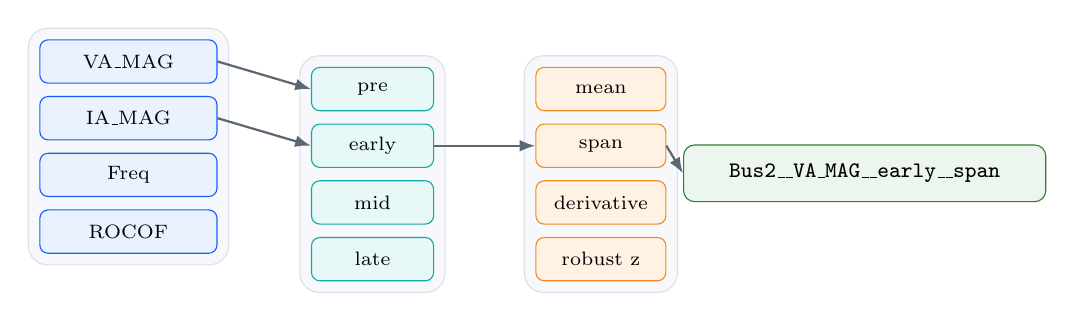
\begin{tikzpicture}[
  sig/.style={rounded corners=3pt,draw=Blue,fill=SoftBlue,minimum width=2.25cm,minimum height=0.55cm,font=\scriptsize},
  seg/.style={rounded corners=3pt,draw=Cyan,fill=SoftCyan,minimum width=1.55cm,minimum height=0.55cm,font=\scriptsize},
  stat/.style={rounded corners=3pt,draw=Orange,fill=SoftOrange,minimum width=1.65cm,minimum height=0.55cm,font=\scriptsize},
  outbox/.style={rounded corners=4pt,draw=Green,fill=SoftGreen,minimum width=4.6cm,minimum height=0.72cm,font=\scriptsize},
  arrow/.style={-{Latex[length=2mm]},thick,draw=Muted}
]
\node[sig] (s1) at (0,1.5) {VA\_MAG};
\node[sig] (s2) at (0,0.78) {IA\_MAG};
\node[sig] (s3) at (0,0.06) {Freq};
\node[sig] (s4) at (0,-0.66) {ROCOF};
\node[seg] (pre) at (3.1,1.15) {pre};
\node[seg] (early) at (3.1,0.43) {early};
\node[seg] (mid) at (3.1,-0.29) {mid};
\node[seg] (late) at (3.1,-1.01) {late};
\node[stat] (mean) at (6.0,1.15) {mean};
\node[stat] (span) at (6.0,0.43) {span};
\node[stat] (der) at (6.0,-0.29) {derivative};
\node[stat] (z) at (6.0,-1.01) {robust z};
\node[outbox] (out) at (9.35,0.08) {\code{Bus2\_\_VA\_MAG\_\_early\_\_span}};
\draw[arrow] (s1.east) -- (pre.west);
\draw[arrow] (s2.east) -- (early.west);
\draw[arrow] (early.east) -- (span.west);
\draw[arrow] (span.east) -- (out.west);
\begin{scope}[on background layer]
  \node[rounded corners=7pt,draw=Line,fill=Paper,fit=(s1)(s4),inner sep=4pt] {};
  \node[rounded corners=7pt,draw=Line,fill=Paper,fit=(pre)(late),inner sep=4pt] {};
  \node[rounded corners=7pt,draw=Line,fill=Paper,fit=(mean)(z),inner sep=4pt] {};
\end{scope}
\end{tikzpicture}
\vspace{3mm}
\begin{block}{Reimplementation shortcut}
Write the extractor as nested loops: for each PMU, for each signal, for each segment, compute the same statistics with the same names.
\end{block}
\end{frame}

% -------------------------------------------------------------------
\begin{frame}{Statistics generated inside each segment}
\small
\begin{columns}[T,totalwidth=\textwidth]
\begin{column}{0.49\textwidth}
\begin{block}{For centered values $\tilde{x}(t)$ in segment $\mathcal{S}$}
\[
\mu_{\mathcal{S}}=\frac{1}{|\mathcal{S}|}\sum_{t\in\mathcal{S}}\tilde{x}(t)
\]
\[
\sigma_{\mathcal{S}}=
\sqrt{\frac{1}{|\mathcal{S}|}\sum_{t\in\mathcal{S}}
\left(\tilde{x}(t)-\mu_{\mathcal{S}}\right)^2}
\]
\[
\mathrm{span}_{\mathcal{S}}=
\max_{t\in\mathcal{S}}\tilde{x}(t)-
\min_{t\in\mathcal{S}}\tilde{x}(t)
\]
\end{block}
\end{column}
\begin{column}{0.47\textwidth}
\begin{exampleblock}{Also stored}
\[
\min,\ \max,\ \mathrm{median},\ \max|\tilde{x}|,\ 
\mathrm{mean}|\tilde{x}|,\ p05,\ p95
\]
\end{exampleblock}
\centering
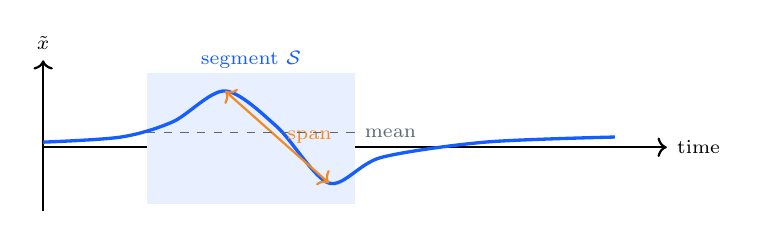
\begin{tikzpicture}[x=0.33cm,y=0.65cm]
  \draw[->,thick] (0,0) -- (24,0) node[right]{\scriptsize time};
  \draw[->,thick] (0,-1.25) -- (0,1.7) node[above]{\scriptsize $\tilde{x}$};
  \fill[Blue!10] (4,-1.1) rectangle (12,1.45);
  \node[Blue] at (8,1.7) {\scriptsize segment $\mathcal{S}$};
  \draw[Blue,very thick,smooth] plot coordinates {(0,0.1)(3,0.2)(5,0.5)(7,1.1)(9,0.4)(11,-0.7)(13,-0.2)(17,0.1)(22,0.2)};
  \draw[Orange,<->,thick] (11,-0.7) -- (7,1.1) node[midway,right]{\scriptsize span};
  \draw[Muted,dashed] (4,0.28) -- (12,0.28) node[right]{\scriptsize mean};
\end{tikzpicture}
\end{column}
\end{columns}
\end{frame}

% -------------------------------------------------------------------

% -------------------------------------------------------------------

% -------------------------------------------------------------------
\fi
\begin{frame}{Temporal deltas and derivative features}
\small
\begin{columns}[T,totalwidth=\textwidth]
\begin{column}{0.50\textwidth}
\begin{block}{Definitions}
\[
\Delta_{\mathrm{early}}=\mu_{\mathrm{early}}-\mu_{\mathrm{pre}}
\]
\[
\Delta_{\mathrm{mid}}=\mu_{\mathrm{mid}}-\mu_{\mathrm{pre}}
\]
\[
\Delta_{\mathrm{late}}=\mu_{\mathrm{late}}-\mu_{\mathrm{pre}}
\]
\end{block}
\end{column}
\begin{column}{0.46\textwidth}
\begin{exampleblock}{Interpretation}
\begin{itemize}
  \item early delta: onset shock.
  \item mid delta: transient settling.
  \item late delta: persistent operating-point change.
\end{itemize}
\end{exampleblock}
\end{column}
\end{columns}
\vspace{2mm}
\begin{alertblock}{Derivative features}
\[
d_x(t)=\frac{x(t)-x(t-\Delta t)}{\Delta t},\qquad
\max_t |d_x(t)|,\qquad
\sqrt{T^{-1}\sum_t d_x(t)^2}
\]
Large voltage/current derivatives flag abrupt transients used by the fault and line-outage guards.
\end{alertblock}
\end{frame}

% -------------------------------------------------------------------
\iffalse
\begin{frame}{3. Derivative features}
\small
\begin{block}{Finite-difference approximation}
\[
d_x(t) = \frac{x(t)-x(t-\Delta t)}{\Delta t}
\]
\[
\mathrm{max\_abs\_derivative}=\max_t |d_x(t)|,\qquad
\mathrm{rms\_derivative}=\sqrt{\frac{1}{T}\sum_t d_x(t)^2}
\]
\end{block}
\begin{columns}[T,totalwidth=\textwidth]
\begin{column}{0.47\textwidth}
\begin{exampleblock}{High derivative}
Usually means an abrupt transient: fault onset, line switching, or corrupted data.
\end{exampleblock}
\end{column}
\begin{column}{0.49\textwidth}
\begin{alertblock}{Event use}
The final rule engine uses voltage and current derivative thresholds to guard fault and line-outage decisions.
\end{alertblock}
\end{column}
\end{columns}
\end{frame}

% -------------------------------------------------------------------

% -------------------------------------------------------------------
\fi
\begin{frame}{Robust z-score separates two failure modes}
\small
\begin{columns}[T,totalwidth=\textwidth]
\begin{column}{0.50\textwidth}
\centering
\resizebox{\linewidth}{!}{%
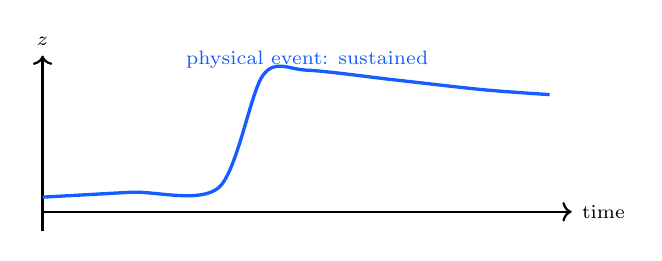
\begin{tikzpicture}[x=0.28cm,y=0.62cm]
  \draw[->,thick] (0,0) -- (24,0) node[right]{\scriptsize time};
  \draw[->,thick] (0,-0.4) -- (0,3.2) node[above]{\scriptsize $z$};
  \draw[Blue,very thick,smooth] plot coordinates {(0,0.3)(4,0.4)(8,0.5)(10,2.8)(12,2.9)(16,2.7)(20,2.5)(23,2.4)};
  \node[Blue] at (12,3.12) {\scriptsize physical event: sustained};
\end{tikzpicture}}\\[1mm]
\resizebox{\linewidth}{!}{%
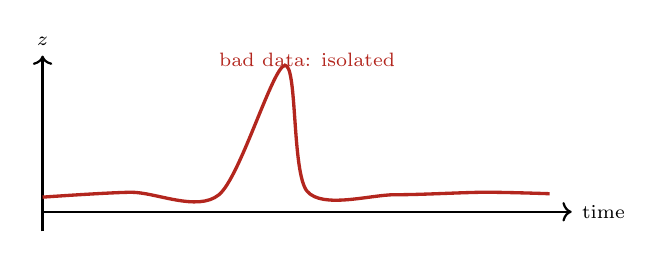
\begin{tikzpicture}[x=0.28cm,y=0.62cm]
  \draw[->,thick] (0,0) -- (24,0) node[right]{\scriptsize time};
  \draw[->,thick] (0,-0.4) -- (0,3.2) node[above]{\scriptsize $z$};
  \draw[Red,very thick,smooth] plot coordinates {(0,0.3)(4,0.4)(8,0.35)(11,3.0)(12,0.42)(16,0.35)(20,0.40)(23,0.37)};
  \node[Red] at (12,3.12) {\scriptsize bad data: isolated};
\end{tikzpicture}}
\end{column}
\begin{column}{0.46\textwidth}
\begin{block}{Peak and persistence}
\code{max\_abs\_robust\_z} catches the spike. Sustained features say whether the abnormal value stays high for several samples.
\end{block}
\begin{alertblock}{Classifier use}
\code{sustained\_abs\_robust\_z\_5} and \code{sustained\_abs\_robust\_z\_15} separate short bursts, persistent physical deviations, and isolated bad-data spikes.
\end{alertblock}
\end{column}
\end{columns}
\end{frame}

% -------------------------------------------------------------------
\iffalse
\begin{frame}{5. Sustained anomaly features}
\small
\begin{block}{Concept}
Not every high z-score is equally meaningful. A single spike may be bad data; a sustained high z-score may be a physical event.
\end{block}
\begin{columns}[T,totalwidth=\textwidth]
\begin{column}{0.48\textwidth}
\begin{exampleblock}{Short sustained score}
\code{sustained\_abs\_robust\_z\_5}\\
Captures short bursts and sharp events.
\end{exampleblock}
\end{column}
\begin{column}{0.48\textwidth}
\begin{exampleblock}{Long sustained score}
\code{sustained\_abs\_robust\_z\_15}\\
Captures persistent deviations after the event.
\end{exampleblock}
\end{column}
\end{columns}
\vspace{2mm}
\begin{alertblock}{Anomaly interpretation}
Faults can be sharp and sustained; bad data is often isolated to one channel; load/generation changes persist in late features.
\end{alertblock}
\end{frame}

% -------------------------------------------------------------------
\fi
\begin{frame}{Data quality, bad data, and phase consistency}
\small
\begin{columns}[T,totalwidth=\textwidth]
\begin{column}{0.53\textwidth}
\begin{block}{Missing-data features}
\begin{itemize}
  \item \code{n\_samples}, \code{duration\_s}, \code{dt\_s}
  \item \code{max\_timestamp\_gap\_s}, \code{max\_timestamp\_gap\_ratio}
  \item \code{data\_present\_fraction}, \code{data\_present\_min}
  \item \code{missing\_run\_max\_samples/s}
  \item \code{nan\_fraction\_max/mean}
\end{itemize}
\end{block}
\begin{alertblock}{Missing route}
Missing only $\rightarrow$ Event 5. Missing plus physical evidence $\rightarrow$ Event 6.
\end{alertblock}
\end{column}
\begin{column}{0.43\textwidth}
\begin{exampleblock}{Bad-data score}
\[
\frac{\mathrm{top\ anomaly}}{\mathrm{second\ anomaly}}\ge3
\Rightarrow \mathrm{bad\ data}
\]
\end{exampleblock}
\begin{block}{Phase consistency}
Phase-to-phase spread and angle coherence separate grid events from corrupted single channels.
\end{block}
\end{column}
\end{columns}
\end{frame}

% -------------------------------------------------------------------
\iffalse
\begin{frame}{7. Single-signal bad-data features}
\small
\begin{block}{Goal}
Detect a channel that becomes extreme while the rest of the PMU/grid remains coherent.
\end{block}
\begin{columns}[T,totalwidth=\textwidth]
\begin{column}{0.50\textwidth}
\begin{exampleblock}{Features}
\begin{itemize}
  \item \code{single\_signal\_score\_max}
  \item \code{single\_signal\_score\_second}
  \item \code{single\_signal\_score\_ratio}
  \item \code{single\_signal\_score\_count\_gt20}
\end{itemize}
\end{exampleblock}
\end{column}
\begin{column}{0.46\textwidth}
\begin{alertblock}{Rule of thumb}
\[
\frac{\mathrm{top\ anomaly}}{\mathrm{second\ anomaly}} \ge 3
\Rightarrow \mathrm{bad\ data\ candidate}
\]
\end{alertblock}
\end{column}
\end{columns}
\end{frame}

% -------------------------------------------------------------------
\begin{frame}{8. Phase-spread and consistency features}
\small
\begin{block}{Measured quantity}
For voltage/current magnitude and angle groups, the extractor summarizes phase-to-phase spread and consistency.
\end{block}
\begin{columns}[T,totalwidth=\textwidth]
\begin{column}{0.48\textwidth}
\begin{exampleblock}{Physical role}
\begin{itemize}
  \item three-phase imbalance,
  \item phase-angle inconsistency,
  \item PMU channel mismatch.
\end{itemize}
\end{exampleblock}
\end{column}
\begin{column}{0.48\textwidth}
\begin{alertblock}{Event use}
These features separate grid events from measurement artifacts because real events tend to preserve more cross-phase structure than corrupted channels.
\end{alertblock}
\end{column}
\end{columns}
\end{frame}

% -------------------------------------------------------------------
\fi
\begin{frame}{Power proxy, global aggregation, and base count}
\scriptsize
\begin{columns}[T,totalwidth=\textwidth]
\begin{column}{0.47\textwidth}
\begin{block}{Per-unit magnitudes}
\[
V_{pu,\phi}(t)=
\frac{|V_{\phi}(t)|}
{\max(\mathrm{median}_{pre}|V_{\phi}|,\epsilon)}
\]
\[
I_{pu,\phi}(t)=
\frac{|I_{\phi}(t)|}
{\max(\mathrm{median}_{pre}|I_{\phi}|,\epsilon)}
\]
\end{block}
\begin{alertblock}{Proxy, not calibrated power}
The challenge data does not require a full power-flow solve. Sign depends on the PMU current convention, but the proxy gives the classifier a stable active/reactive signature.
\end{alertblock}
\end{column}
\begin{column}{0.49\textwidth}
\centering
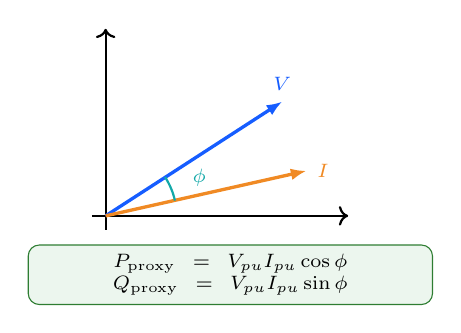
\begin{tikzpicture}[scale=0.88]
  \draw[->,thick] (-0.2,0) -- (3.5,0);
  \draw[->,thick] (0,-0.2) -- (0,2.7);
  \draw[Blue,very thick,-{Latex[length=2mm]}] (0,0) -- (2.55,1.65) node[above]{\scriptsize $V$};
  \draw[Orange,very thick,-{Latex[length=2mm]}] (0,0) -- (2.9,0.65) node[right]{\scriptsize $I$};
  \draw[Cyan,thick] (1.0,0.22) arc[start angle=12.6,end angle=32.9,radius=1.05];
  \node[Cyan] at (1.35,0.55) {\scriptsize $\phi$};
  \node[rounded corners=4pt,draw=Green,fill=SoftGreen,text width=4.9cm,align=center,font=\scriptsize] at (1.8,-0.85)
  {$P_{\mathrm{proxy}}=V_{pu}I_{pu}\cos\phi$\\$Q_{\mathrm{proxy}}=V_{pu}I_{pu}\sin\phi$};
\end{tikzpicture}
\vspace{-1mm}
\begin{exampleblock}{Global summaries and count}
Stores cross-PMU \(\mathrm{mean},\max,\min,\mathrm{std}\). Base statistical total: \(\mathbf{39{,}744}\) features.
\end{exampleblock}
\end{column}
\end{columns}
\end{frame}

% -------------------------------------------------------------------

% -------------------------------------------------------------------
\iffalse
\begin{frame}{10. Global PMU aggregation}
\small
\begin{block}{Aggregated quantities}
After extracting bus-level features, the model also computes global summaries across observed PMUs:
\[
\mathrm{mean},\ \mathrm{max},\ \mathrm{min},\ \mathrm{std}
\]
\end{block}
\begin{exampleblock}{System footprint}
A local event has a spatial footprint. Global aggregation gives the classifier a system-level view: is the disturbance concentrated, widespread, coherent, or isolated?
\end{exampleblock}
\begin{alertblock}{Example}
Bad data often has one extreme PMU/channel. A physical event affects multiple PMUs in a structured way.
\end{alertblock}
\end{frame}

% -------------------------------------------------------------------
\begin{frame}{Base feature count}
\small
\centering
\begin{tabular}{lr}
\toprule
\textbf{Feature group} & \textbf{Count}\\
\midrule
Voltage angle & 7,596\\
Voltage magnitude & 7,596\\
Current angle & 7,596\\
Current magnitude & 7,596\\
Frequency / ROCOF & 4,640\\
Power proxy & 4,428\\
Data quality & 156\\
Single-signal anomaly & 48\\
Other/global and alignment & 88\\
\midrule
\textbf{Base statistical total} & \textbf{39,744}\\
\bottomrule
\end{tabular}
\vspace{3mm}
\begin{block}{Reimplementation note}
The count is large, but the implementation is loop-based: signal family, segment, statistic, then global aggregation.
\end{block}
\end{frame}

% -------------------------------------------------------------------
\fi
\section{Dynamic Feature Engineering}
\sectionframe{}{Dynamic Feature\\Engineering}{Rolling, adaptive-residual, and graph-temporal evidence}


% -------------------------------------------------------------------

% -------------------------------------------------------------------
\begin{frame}{Dynamic features: signals and three views}
\small
\begin{columns}[T,totalwidth=\textwidth]
\begin{column}{0.46\textwidth}
\begin{block}{Signals}
\[
\begin{aligned}
\{&\mathrm{VA\_MAG},\ \mathrm{IA\_MAG},\ \mathrm{VA\_ANG},\\
 &\mathrm{IA\_ANG},\ \mathrm{Freq},\ \mathrm{ROCOF}\}
\end{aligned}
\]
Full magnitude/angle families are used where feasible; the reduced set controls feature count for residual and graph modules.
\end{block}
\end{column}
\begin{column}{0.50\textwidth}
\centering
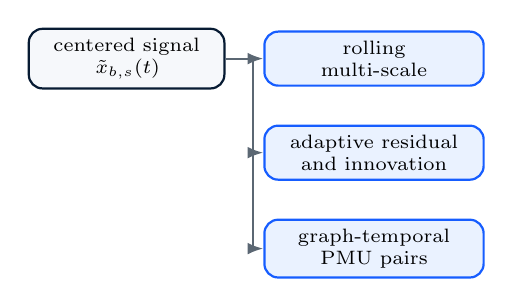
\begin{tikzpicture}[
  node distance=0.48cm,
  raw/.style={rounded corners=5pt,draw=Navy,fill=Paper,thick,text width=2.25cm,minimum height=0.68cm,align=center,font=\scriptsize},
  view/.style={rounded corners=5pt,draw=Blue,fill=SoftBlue,thick,text width=2.55cm,minimum height=0.68cm,align=center,font=\scriptsize},
  arrow/.style={-{Latex[length=2mm]},thick,draw=Muted}
]
\node[raw] (x) {centered signal\\$\tilde{x}_{b,s}(t)$};
\node[view,right=of x] (r) {rolling\\multi-scale};
\node[view,below=of r] (a) {adaptive residual\\and innovation};
\node[view,below=of a] (g) {graph-temporal\\PMU pairs};
\draw[arrow] (x.east) -- (r.west);
\draw[arrow] (x.east) -- ++(0.35,0) |- (a.west);
\draw[arrow] (x.east) -- ++(0.35,0) |- (g.west);
\end{tikzpicture}
\end{column}
\end{columns}
\begin{alertblock}{Purpose}
These modules add time-scale, residual, and spatial-propagation evidence after the base statistics.
\end{alertblock}
\end{frame}

\iffalse
\begin{frame}{Dynamic feature blocks}
\small
\centering
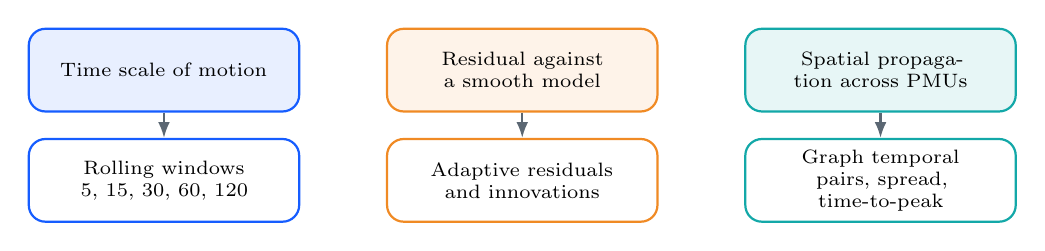
\begin{tikzpicture}[
  qblue/.style={rounded corners=6pt,draw=Blue,fill=Blue!10,thick,text width=3.2cm,minimum height=1.05cm,align=center,font=\scriptsize},
  ablue/.style={rounded corners=6pt,draw=Blue,fill=white,thick,text width=3.2cm,minimum height=1.05cm,align=center,font=\scriptsize},
  qorange/.style={rounded corners=6pt,draw=Orange,fill=Orange!10,thick,text width=3.2cm,minimum height=1.05cm,align=center,font=\scriptsize},
  aorange/.style={rounded corners=6pt,draw=Orange,fill=white,thick,text width=3.2cm,minimum height=1.05cm,align=center,font=\scriptsize},
  qcyan/.style={rounded corners=6pt,draw=Cyan,fill=Cyan!10,thick,text width=3.2cm,minimum height=1.05cm,align=center,font=\scriptsize},
  acyan/.style={rounded corners=6pt,draw=Cyan,fill=white,thick,text width=3.2cm,minimum height=1.05cm,align=center,font=\scriptsize},
  arrow/.style={-{Latex[length=2mm]},thick,draw=Muted}
]
\node[qblue] (q1) at (0,1.4) {Time scale of motion};
\node[ablue] (a1) at (0,0) {Rolling windows\\5, 15, 30, 60, 120};
\node[qorange] (q2) at (4.55,1.4) {Residual against a smooth model};
\node[aorange] (a2) at (4.55,0) {Adaptive residuals\\and innovations};
\node[qcyan] (q3) at (9.1,1.4) {Spatial propagation across PMUs};
\node[acyan] (a3) at (9.1,0) {Graph temporal\\pairs, spread, time-to-peak};
\draw[arrow] (q1) -- (a1);
\draw[arrow] (q2) -- (a2);
\draw[arrow] (q3) -- (a3);
\end{tikzpicture}
\vspace{3mm}
\begin{block}{Implementation}
Each block is a separate feature module applied after base-window extraction.
\end{block}
\end{frame}

% -------------------------------------------------------------------
\begin{frame}{Signals used in dynamic extraction}
\small
\begin{block}{Main signal set}
\[
\{\mathrm{VA/VB/VC\_MAG},\ \mathrm{IA/IB/IC\_MAG},\ \mathrm{VA/VB/VC\_ANG},\ \mathrm{IA/IB/IC\_ANG},\ \mathrm{Freq},\ \mathrm{ROCOF}\}
\]
\end{block}
\begin{exampleblock}{Reduced signal set for residual and graph features}
\[
\{\mathrm{VA\_MAG},\ \mathrm{IA\_MAG},\ \mathrm{VA\_ANG},\ \mathrm{IA\_ANG},\ \mathrm{Freq},\ \mathrm{ROCOF}\}
\]
\end{exampleblock}
\begin{alertblock}{Reason}
The reduced set keeps dynamic features feasible while preserving representative voltage, current, angle, and frequency behavior.
\end{alertblock}
\end{frame}

% -------------------------------------------------------------------
\begin{frame}{Dynamic extractor: same signal, three views}
\small
\centering
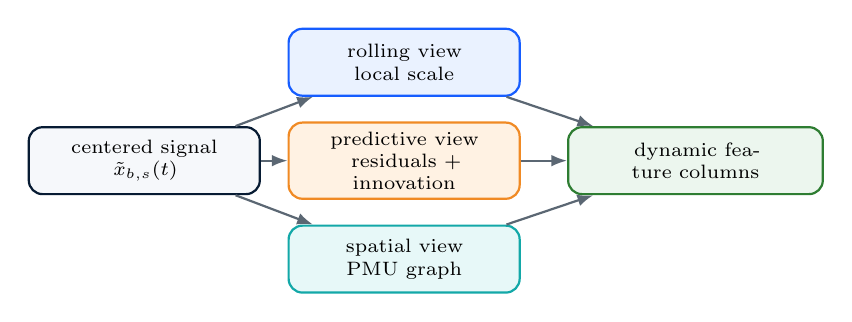
\begin{tikzpicture}[
  node distance=0.75cm,
  raw/.style={rounded corners=5pt,draw=Navy,fill=Paper,thick,text width=2.7cm,minimum height=0.85cm,align=center,font=\scriptsize},
  roll/.style={rounded corners=5pt,draw=Blue,fill=SoftBlue,thick,text width=2.7cm,minimum height=0.85cm,align=center,font=\scriptsize},
  rls/.style={rounded corners=5pt,draw=Orange,fill=SoftOrange,thick,text width=2.7cm,minimum height=0.85cm,align=center,font=\scriptsize},
  graph/.style={rounded corners=5pt,draw=Cyan,fill=SoftCyan,thick,text width=2.7cm,minimum height=0.85cm,align=center,font=\scriptsize},
  outbox/.style={rounded corners=5pt,draw=Green,fill=SoftGreen,thick,text width=3.0cm,minimum height=0.85cm,align=center,font=\scriptsize},
  arrow/.style={-{Latex[length=2mm]},thick,draw=Muted}
]
\node[raw] (x) at (0,0) {centered signal\\$\tilde{x}_{b,s}(t)$};
\node[roll] (r) at (3.3,1.25) {rolling view\\local scale};
\node[rls] (k) at (3.3,0) {predictive view\\residuals + innovation};
\node[graph] (g) at (3.3,-1.25) {spatial view\\PMU graph};
\node[outbox] (f) at (7.0,0) {dynamic feature columns};
\draw[arrow] (x) -- (r);
\draw[arrow] (x) -- (k);
\draw[arrow] (x) -- (g);
\draw[arrow] (r) -- (f);
\draw[arrow] (k) -- (f);
\draw[arrow] (g) -- (f);
\end{tikzpicture}
\vspace{3mm}
\begin{block}{Implementation reading}
All dynamic blocks start after baseline subtraction, which keeps buses and RAW/SIM cases on comparable scales.
\end{block}
\end{frame}

% -------------------------------------------------------------------
\fi
\begin{frame}{Rolling multi-scale features and equations}
\small
\begin{columns}[T,totalwidth=\textwidth]
\begin{column}{0.45\textwidth}
\begin{block}{Rolling windows}
\[
w \in \{5,15,30,60,120\}
\]
\end{block}
\begin{block}{Features}
\begin{itemize}
  \item \code{mean\_abs\_max}
  \item \code{std\_max}, \code{std\_mean}
  \item \code{slope\_max\_abs}
  \item \code{energy}
  \item \code{time\_to\_abs\_peak}
\end{itemize}
\end{block}
\end{column}
\begin{column}{0.51\textwidth}
\begin{block}{Equations}
\[
\mu_w(t)=w^{-1}\sum_{\tau\in W_w(t)}\tilde{x}(\tau)
\]
\[
\sigma_w(t)=\mathrm{std}_{\tau\in W_w(t)}\tilde{x}(\tau)
\]
\[
E_x=T^{-1}\sum_t|\tilde{x}(t)|^2
\]
\end{block}
\begin{exampleblock}{Interpretation}
Short windows capture abrupt switching/fault onset. Long windows capture sustained load/generation shifts. Time-to-peak captures delay.
\end{exampleblock}
\end{column}
\end{columns}
\end{frame}

% -------------------------------------------------------------------
\iffalse
\begin{frame}{Rolling block equations and plot}
\small
\begin{columns}[T,totalwidth=\textwidth]
\begin{column}{0.49\textwidth}
\begin{block}{Centered rolling mean and standard deviation}
\[
\mu_w(t)=\frac{1}{w}\sum_{\tau\in W_w(t)}\tilde{x}(\tau)
\]
\[
\sigma_w(t)=
\sqrt{\frac{1}{w}\sum_{\tau\in W_w(t)}
\left(\tilde{x}(\tau)-\mu_w(t)\right)^2}
\]
\[
E_x=\frac{1}{T}\sum_t|\tilde{x}(t)|^2
\]
\end{block}
\end{column}
\begin{column}{0.47\textwidth}
\centering
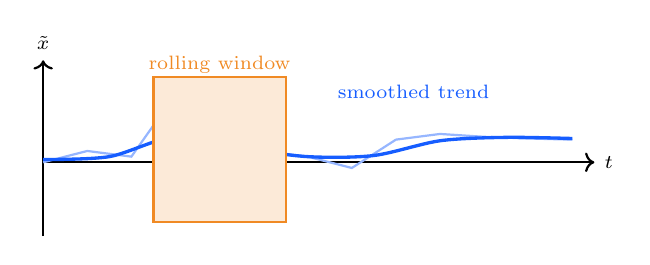
\begin{tikzpicture}[x=0.28cm,y=0.72cm]
  \draw[->,thick] (0,0) -- (25,0) node[right]{\scriptsize $t$};
  \draw[->,thick] (0,-1.3) -- (0,1.8) node[above]{\scriptsize $\tilde{x}$};
  \draw[Blue!45,thick] plot coordinates {(0,0.0)(2,0.2)(4,0.1)(6,1.2)(8,-0.6)(10,0.2)(12,0.1)(14,-0.1)(16,0.4)(18,0.5)(20,0.45)(22,0.42)(24,0.40)};
  \draw[Blue,very thick,smooth] plot coordinates {(0,0.05)(3,0.1)(6,0.45)(9,0.25)(12,0.1)(15,0.12)(18,0.38)(21,0.44)(24,0.42)};
  \fill[Orange!18] (5,-1.05) rectangle (11,1.5);
  \draw[Orange,thick] (5,-1.05) rectangle (11,1.5);
  \node[Orange] at (8,1.72) {\scriptsize rolling window};
  \node[Blue] at (16.8,1.25) {\scriptsize smoothed trend};
\end{tikzpicture}
\vspace{2mm}
\begin{exampleblock}{Stored for each $w$}
\[
\max|\mu_w|,\quad \max\sigma_w,\quad \overline{\sigma_w},\quad
\max\left|\frac{d\mu_w}{dt}\right|,\quad E_x,\quad t_{\mathrm{peak}}
\]
\end{exampleblock}
\end{column}
\end{columns}
\end{frame}

% -------------------------------------------------------------------

% -------------------------------------------------------------------
\fi
\begin{frame}{RLS level and linear-trend residuals}
\small
\begin{columns}[T,totalwidth=\textwidth]
\begin{column}{0.52\textwidth}
\begin{block}{Model}
\[
y_t=\theta_t+e_t
\]
\[
K_t=\frac{P_{t-1}}{\lambda+P_{t-1}}
\]
\[
\theta_t=\theta_{t-1}+K_t(y_t-\theta_{t-1})
\]
\[
P_t=\frac{P_{t-1}-K_tP_{t-1}}{\lambda}
\]
\end{block}
\begin{exampleblock}{Forgetting factors}
\[
\lambda\in\{0.92,\ 0.985\}
\]
\[
\phi_t=[1,\ t-t_0]^T,\quad
\hat{y}_t=\phi_t^T\theta_{t-1}
\]
\end{exampleblock}
\end{column}
\begin{column}{0.44\textwidth}
\begin{alertblock}{Features produced}
\[
r_t=|y_t-\theta_{t-1}|
\]
\[
\Delta\theta_t=|\theta_t-\theta_{t-1}|
\]
For each sequence:
\[
\max,\quad \mathrm{mean},\quad p95,
\]
\[
\mathrm{median}_{late}-\mathrm{median}_{pre}
\]
\end{alertblock}
\centering
\resizebox{\linewidth}{!}{%
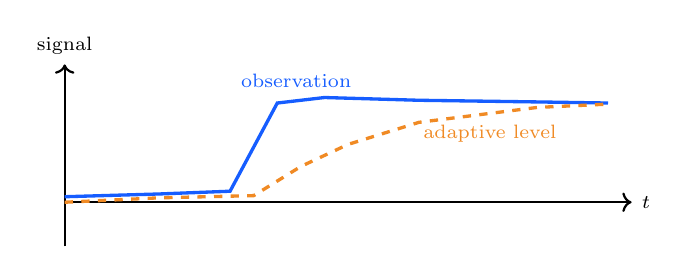
\begin{tikzpicture}[x=0.30cm,y=0.70cm]
  \draw[->,thick] (0,0) -- (24,0) node[right]{\scriptsize $t$};
  \draw[->,thick] (0,-0.8) -- (0,2.5) node[above]{\scriptsize signal};
  \draw[Blue,very thick] plot coordinates {(0,0.1)(4,0.15)(7,0.2)(9,1.8)(11,1.9)(15,1.85)(20,1.82)(23,1.8)};
  \draw[Orange,very thick,dashed] plot coordinates {(0,0.0)(4,0.08)(8,0.12)(10,0.65)(12,1.05)(15,1.45)(20,1.72)(23,1.78)};
  \node[Blue] at (9.8,2.2) {\scriptsize observation};
  \node[Orange] at (18,1.25) {\scriptsize adaptive level};
\end{tikzpicture}}
\end{column}
\end{columns}
\end{frame}

% -------------------------------------------------------------------
\iffalse
\begin{frame}{RLS linear-trend model}
\small
\begin{columns}[T,totalwidth=\textwidth]
\begin{column}{0.53\textwidth}
\begin{block}{Local linear predictor}
\[
\phi_t=\begin{bmatrix}1\\t-t_0\end{bmatrix},
\qquad
\hat{y}_t=\phi_t^\top\theta_{t-1}
\]
\[
K_t=\frac{P_{t-1}\phi_t}
{\lambda+\phi_t^\top P_{t-1}\phi_t}
\]
\[
\theta_t=\theta_{t-1}+K_t(y_t-\hat{y}_t)
\]
\[
P_t=\frac{P_{t-1}-K_t\phi_t^\top P_{t-1}}{\lambda}
\]
\end{block}
\end{column}
\begin{column}{0.43\textwidth}
\centering
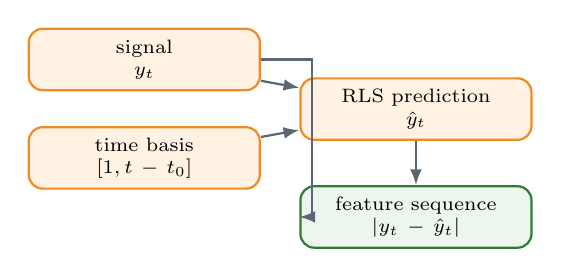
\begin{tikzpicture}[
  box/.style={rounded corners=5pt,draw=Orange,fill=SoftOrange,thick,text width=2.7cm,minimum height=0.78cm,align=center,font=\scriptsize},
  outbox/.style={rounded corners=5pt,draw=Green,fill=SoftGreen,thick,text width=2.7cm,minimum height=0.78cm,align=center,font=\scriptsize},
  arrow/.style={-{Latex[length=2mm]},thick,draw=Muted}
]
\node[box] (x) at (0,1.35) {signal\\$y_t$};
\node[box] (phi) at (0,0.1) {time basis\\$[1,t-t_0]$};
\node[box] (pred) at (3.45,0.72) {RLS prediction\\$\hat{y}_t$};
\node[outbox] (res) at (3.45,-0.65) {feature sequence\\$|y_t-\hat{y}_t|$};
\draw[arrow] (x) -- (pred);
\draw[arrow] (phi) -- (pred);
\draw[arrow] (pred) -- (res);
\draw[arrow] (x.east) -- ++(0.65,0) |- (res.west);
\end{tikzpicture}
\vspace{3mm}
\begin{exampleblock}{Linear residual signal}
They discount smooth ramps but react to switching, faults, and sudden sensor errors.
\end{exampleblock}
\end{column}
\end{columns}
\end{frame}

% -------------------------------------------------------------------
\fi
\begin{frame}{Adaptive innovation filter}
\small
\begin{columns}[T,totalwidth=\textwidth]
\begin{column}{0.52\textwidth}
\begin{block}{Smooth level model}
\[
x_t=x_{t-1}+w_t,\qquad w_t\sim\mathcal{N}(0,Q)
\]
\[
y_t=x_t+v_t,\qquad v_t\sim\mathcal{N}(0,R)
\]
\[
Q=(0.005\,s)^2,\qquad R=(0.08\,s)^2
\]
\[
s=\mathrm{robust\_scale}(y)
\]
\end{block}
\end{column}
\begin{column}{0.44\textwidth}
\begin{alertblock}{Innovation update}
\[
P_t^- = P_{t-1}+Q
\]
\[
\nu_t=y_t-\hat{x}_{t-1}
\]
\[
K_t=\frac{P_t^-}{P_t^-+R}
\]
\[
\hat{x}_t=\hat{x}_{t-1}+K_t\nu_t,\qquad
P_t=(1-K_t)P_t^-
\]
\end{alertblock}
\end{column}
\end{columns}
\vspace{1mm}
\begin{exampleblock}{Stored features and event use}
\[
\max|\nu_t|,\quad \mathrm{mean}|\nu_t|,\quad p95|\nu_t|,\quad t_{\mathrm{peak}}
\]
Useful for Event 1, Event 2, and Event 8 localization; Events 3--4 use it when the change is gradual but persistent.
\end{exampleblock}
\end{frame}

% -------------------------------------------------------------------
\iffalse
\begin{frame}{Innovation filter diagram}
\small
\begin{columns}[T,totalwidth=\textwidth]
\begin{column}{0.53\textwidth}
\centering
\resizebox{\linewidth}{!}{%
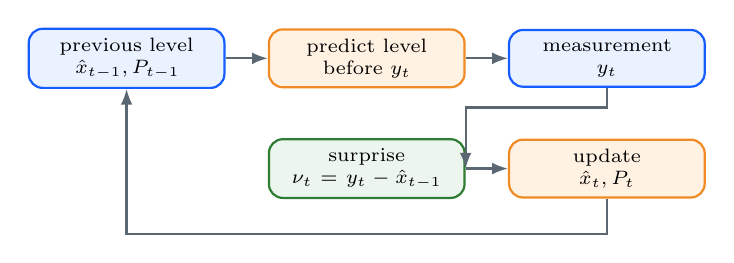
\begin{tikzpicture}[
  box/.style={rounded corners=5pt,draw=Blue,fill=SoftBlue,thick,text width=2.25cm,minimum height=0.72cm,align=center,font=\scriptsize},
  box2/.style={rounded corners=5pt,draw=Orange,fill=SoftOrange,thick,text width=2.25cm,minimum height=0.72cm,align=center,font=\scriptsize},
  box3/.style={rounded corners=5pt,draw=Green,fill=SoftGreen,thick,text width=2.25cm,minimum height=0.72cm,align=center,font=\scriptsize},
  arrow/.style={-{Latex[length=2mm]},thick,draw=Muted}
]
\node[box] (prev) at (0,1.35) {previous level\\$\hat{x}_{t-1},P_{t-1}$};
\node[box2] (pred) at (3.05,1.35) {predict level\\before $y_t$};
\node[box] (meas) at (6.10,1.35) {measurement\\$y_t$};
\node[box3] (innov) at (3.05,-0.05) {surprise\\$\nu_t=y_t-\hat{x}_{t-1}$};
\node[box2] (upd) at (6.10,-0.05) {update\\$\hat{x}_t,P_t$};
\draw[arrow] (prev) -- (pred);
\draw[arrow] (pred) -- (meas);
\draw[arrow] (meas.south) -- ++(0,-0.25) -| (innov.east);
\draw[arrow] (innov) -- (upd);
\draw[arrow] (upd.south) -- ++(0,-0.45) -| (prev.south);
\end{tikzpicture}
}
\end{column}
\begin{column}{0.43\textwidth}
\centering
\resizebox{\linewidth}{!}{%
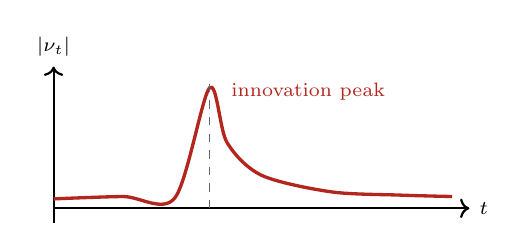
\begin{tikzpicture}[x=0.22cm,y=0.60cm]
  \draw[->,thick] (0,0) -- (24,0) node[right]{\scriptsize $t$};
  \draw[->,thick] (0,-0.3) -- (0,3.0) node[above]{\scriptsize $|\nu_t|$};
  \draw[Red,very thick,smooth] plot coordinates {(0,0.2)(4,0.25)(7,0.22)(9,2.55)(10,1.4)(12,0.7)(16,0.35)(20,0.28)(23,0.25)};
  \draw[Muted,dashed] (9,0) -- (9,2.65);
  \node[Red,anchor=west] at (9.7,2.48) {\scriptsize innovation peak};
\end{tikzpicture}
}
\vspace{2mm}
\begin{exampleblock}{Stored features}
\[
\max|\nu_t|,\quad \mathrm{mean}|\nu_t|,\quad p95|\nu_t|,\quad
t_{\mathrm{peak}}
\]
\end{exampleblock}
\end{column}
\end{columns}
\end{frame}

% -------------------------------------------------------------------
\begin{frame}{Why keep residuals and innovation}
\small
\begin{columns}[T,totalwidth=\textwidth]
\begin{column}{0.49\textwidth}
\centering
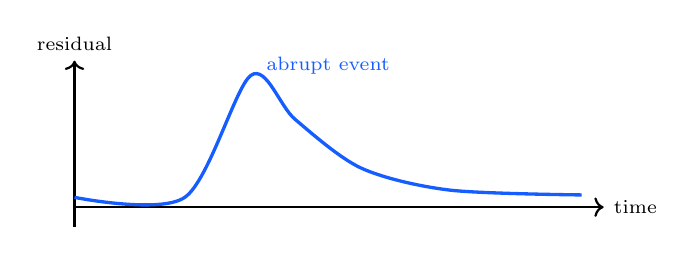
\begin{tikzpicture}[x=0.28cm,y=0.62cm]
  \draw[->,thick] (0,0) -- (24,0) node[right]{\scriptsize time};
  \draw[->,thick] (0,-0.4) -- (0,3.0) node[above]{\scriptsize residual};
  \draw[Blue,very thick,smooth] plot coordinates {(0,0.2)(5,0.2)(8,2.7)(10,1.8)(13,0.8)(17,0.35)(23,0.25)};
  \node[Blue] at (11.5,2.9) {\scriptsize abrupt event};
\end{tikzpicture}\\[2mm]
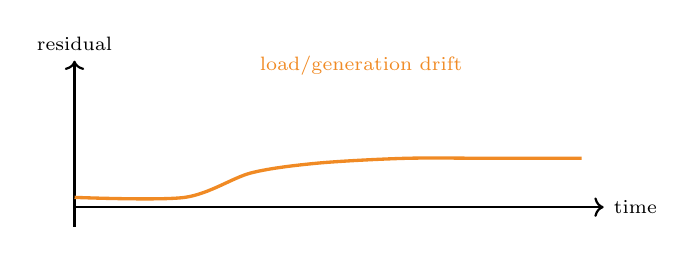
\begin{tikzpicture}[x=0.28cm,y=0.62cm]
  \draw[->,thick] (0,0) -- (24,0) node[right]{\scriptsize time};
  \draw[->,thick] (0,-0.4) -- (0,3.0) node[above]{\scriptsize residual};
  \draw[Orange,very thick,smooth] plot coordinates {(0,0.2)(5,0.2)(8,0.7)(11,0.9)(15,1.0)(19,1.0)(23,1.0)};
  \node[Orange] at (13,2.9) {\scriptsize load/generation drift};
\end{tikzpicture}
\end{column}
\begin{column}{0.47\textwidth}
\begin{block}{Different residual views}
\begin{itemize}
  \item RLS level residual catches sudden level mismatch.
  \item RLS linear residual ignores smooth ramps and exposes abrupt breaks.
  \item Innovation peak gives a noise-scaled one-step surprise.
\end{itemize}
\end{block}
\begin{alertblock}{Event use}
Most useful for Event 1, Event 2, and Event 8 localization; contributes to Events 3--4 when the change is gradual but persistent.
\end{alertblock}
\end{column}
\end{columns}
\end{frame}

% -------------------------------------------------------------------
\fi
\iffalse
\begin{frame}{Non-selected swing-residual branch}
\small
\begin{columns}[T,totalwidth=\textwidth]
\begin{column}{0.52\textwidth}
\begin{block}{Classical generator intuition}
\[
\dot{\delta}=\omega-\omega_0
\]
\[
M\dot{\omega}=P_m-P_e-D(\omega-\omega_0)
\]
\end{block}
\begin{exampleblock}{Branch objective}
Use a light swing-equation residual to capture frequency and angle oscillations after generation/load disturbances.
\end{exampleblock}
\end{column}
\begin{column}{0.44\textwidth}
\centering
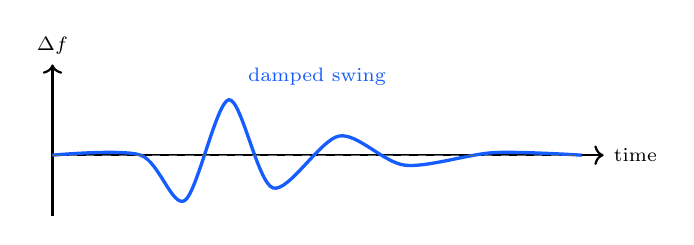
\begin{tikzpicture}[x=0.28cm,y=0.64cm]
  \draw[->,thick] (0,0) -- (25,0) node[right]{\scriptsize time};
  \draw[->,thick] (0,-1.2) -- (0,1.8) node[above]{\scriptsize $\Delta f$};
  \draw[Blue,very thick,smooth] plot coordinates {(0,0)(4,0)(6,-0.9)(8,1.1)(10,-0.65)(13,0.38)(16,-0.2)(20,0.05)(24,0.0)};
  \draw[Muted,dashed] (0,0) -- (24,0);
  \node[Blue] at (12,1.55) {\scriptsize damped swing};
\end{tikzpicture}
\vspace{2mm}
\begin{alertblock}{Selection result}
It improved some synthetic validation behavior but reduced RAW0001 localization. The submitted route kept the simpler adaptive residual and innovation block.
\end{alertblock}
\end{column}
\end{columns}
\end{frame}

% -------------------------------------------------------------------

% -------------------------------------------------------------------
\fi
\begin{frame}{Graph-temporal features and decision form}
\small
\begin{columns}[T,totalwidth=\textwidth]
\begin{column}{0.52\textwidth}
\begin{block}{For signal $s$ and observed buses $\mathcal{B}$}
\[
\mathrm{spread}_s(t)=
\max_{b\in\mathcal{B}}\tilde{x}_{b,s}(t)
-
\min_{b\in\mathcal{B}}\tilde{x}_{b,s}(t)
\]
\[
\Delta_{ab,s}^{max}=\max_t|\tilde{x}_{a,s}(t)-\tilde{x}_{b,s}(t)|
\]
\[
\rho_{ab,s}=\mathrm{corr}(\tilde{x}_{a,s},\tilde{x}_{b,s})
\]
\[
\Delta t^{peak}_{ab,s}=
\left|t^{peak}_{a,s}-t^{peak}_{b,s}\right|
\]
\end{block}
\end{column}
\begin{column}{0.44\textwidth}
\begin{alertblock}{Electrical weighting}
\[
w_{ab}=\frac{1}{\max(d^{eff}_{ab},10^{-5})}
\]
\[
G_s^{max}=\max_{a<b}
w_{ab}\Delta_{ab,s}^{max}
\]
\end{alertblock}
\begin{exampleblock}{Decision form}
\[
x_{\mathrm{loc}}=[x_{\mathrm{base}},x_{\mathrm{dyn}},G]
\]
\[
\hat{\ell}=\arg\max_{\ell}p_{\mathrm{ET}}(\ell\mid x_{\mathrm{loc}})
\]
Graph equations create columns; ExtraTrees learns the thresholds and pair combinations.
\end{exampleblock}
\end{column}
\end{columns}
\end{frame}

% -------------------------------------------------------------------
\begin{frame}{Graph-temporal localization illustration}
\scriptsize
\begin{columns}[T,totalwidth=\textwidth]
\begin{column}{0.56\textwidth}
\centering
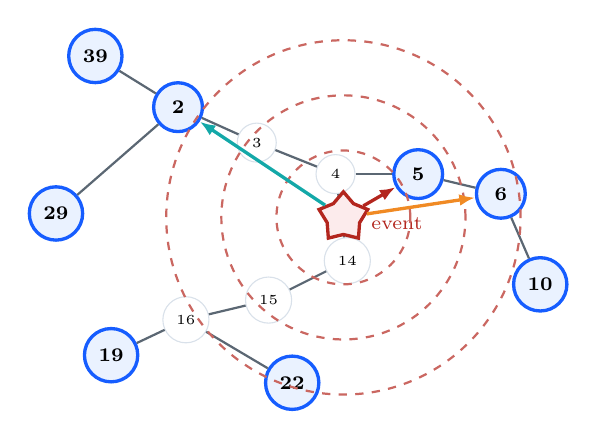
\begin{tikzpicture}[
  pmu/.style={circle,draw=Blue,fill=SoftBlue,very thick,minimum size=0.62cm,font=\scriptsize\bfseries},
  bus/.style={circle,draw=Line,fill=white,minimum size=0.42cm,font=\tiny},
  event/.style={star,star points=5,draw=Red,fill=SoftRed,very thick,minimum size=0.65cm},
  line/.style={draw=Muted,thick},
  pulse/.style={draw=Red!70,dashed,thick}
]
\node[pmu] (b2) at (0,1.7) {2};
\node[bus] (b3) at (1.0,1.25) {3};
\node[bus] (b4) at (2.0,0.85) {4};
\node[pmu] (b5) at (3.05,0.85) {5};
\node[pmu] (b6) at (4.1,0.6) {6};
\node[pmu] (b10) at (4.6,-0.55) {10};
\node[bus] (b14) at (2.15,-0.25) {14};
\node[bus] (b15) at (1.15,-0.75) {15};
\node[bus] (b16) at (0.1,-1.0) {16};
\node[pmu] (b19) at (-0.85,-1.45) {19};
\node[pmu] (b22) at (1.45,-1.8) {22};
\node[pmu] (b29) at (-1.55,0.35) {29};
\node[pmu] (b39) at (-1.05,2.35) {39};
\foreach \a/\b in {b39/b2,b2/b3,b3/b4,b4/b5,b5/b6,b6/b10,b4/b14,b14/b15,b15/b16,b16/b19,b16/b22,b2/b29} {
  \draw[line] (\a) -- (\b);
}
\node[event] (ev) at (2.1,0.3) {};
\node[Red] at (2.78,0.22) {\scriptsize event};
\draw[pulse] (ev) circle (0.85);
\draw[pulse] (ev) circle (1.55);
\draw[pulse] (ev) circle (2.25);
\draw[Red,very thick,-{Latex[length=2mm]}] (ev) -- (b5);
\draw[Orange,very thick,-{Latex[length=2mm]}] (ev) -- (b6);
\draw[Cyan,very thick,-{Latex[length=2mm]}] (ev) -- (b2);
\end{tikzpicture}
\end{column}
\begin{column}{0.40\textwidth}
\begin{block}{Nearby PMU signature}
Larger amplitude, earlier peak, and stronger correlation with electrically close PMUs.
\end{block}
\begin{exampleblock}{Remote PMU signature}
Smaller response, delayed peak, or lower pairwise coherence.
\end{exampleblock}
\begin{alertblock}{Line outage reading}
Event 2 localizes the line whose candidates match current redistribution and graph-difference pattern.
\end{alertblock}
\end{column}
\end{columns}
\end{frame}

% -------------------------------------------------------------------
\iffalse
\begin{frame}{Line outages require graph features}
\small
\begin{columns}[T,totalwidth=\textwidth]
\begin{column}{0.50\textwidth}
\centering
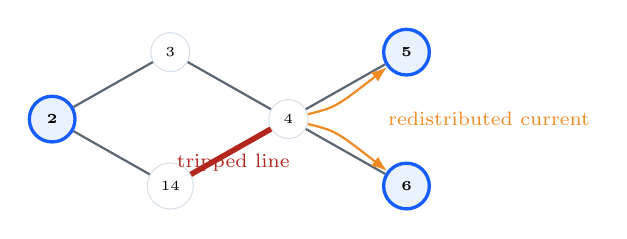
\begin{tikzpicture}[
  bus/.style={circle,draw=Line,fill=white,minimum size=0.48cm,font=\tiny},
  pmu/.style={circle,draw=Blue,fill=SoftBlue,very thick,minimum size=0.58cm,font=\tiny\bfseries},
  outage/.style={draw=Red,line width=2.0pt},
  line/.style={draw=Muted,thick},
  arrow/.style={-{Latex[length=2mm]},thick,draw=Orange}
]
\node[pmu] (a) at (0,0) {2};
\node[bus] (b) at (1.5,0.85) {3};
\node[bus] (c) at (3.0,0) {4};
\node[pmu] (d) at (4.5,0.85) {5};
\node[pmu] (e) at (4.5,-0.85) {6};
\node[bus] (f) at (1.5,-0.85) {14};
\draw[line] (a)--(b)--(c)--(d);
\draw[line] (c)--(e);
\draw[outage] (c)--(f);
\draw[line] (f)--(a);
\draw[arrow] (c) .. controls (3.6,0.15) .. (d);
\draw[arrow] (c) .. controls (3.6,-0.15) .. (e);
\node[Red] at (2.3,-0.55) {\scriptsize tripped line};
\node[Orange] at (5.55,0.0) {\scriptsize redistributed current};
\end{tikzpicture}
\end{column}
\begin{column}{0.46\textwidth}
\begin{block}{Electrical effect}
Opening one line changes current paths. Voltage may not collapse like a fault, but current magnitude, current angle, and pairwise PMU differences move in a structured way.
\end{block}
\begin{alertblock}{Feature consequence}
Event 2 benefits from graph differences, time-to-peak differences, and current-angle/current-magnitude signatures more than from a single largest voltage sag.
\end{alertblock}
\end{column}
\end{columns}
\end{frame}

% -------------------------------------------------------------------
\fi
\begin{frame}{Selected feature variant}
\small
\begin{columns}[T,totalwidth=\textwidth]
\begin{column}{0.46\textwidth}
\begin{block}{Selected}
\centering
{\scriptsize\texttt{base statistical + rolling}}\\[-1mm]
{\scriptsize\texttt{+ adaptive residual + graph-temporal}}\\[1mm]
\[
n_{\mathrm{features}} = 45{,}162
\]
\end{block}
\end{column}
\begin{column}{0.50\textwidth}
\begin{alertblock}{Not selected}
\begin{itemize}
  \item Algebraic residual branch: matched RAW0001 but did not improve it.
  \item Swing-residual branch: improved SIM slightly, reduced RAW0001 localization.
  \item oracle topology ranker: higher RAW0001, but not deployable.
\end{itemize}
\end{alertblock}
\end{column}
\end{columns}
\vspace{2mm}
\begin{exampleblock}{Selection criterion}
RAW0001 Top-1 localization = 0.6667, tied with the best deployable variants; SIM Top-1 localization = 0.8524.
\end{exampleblock}
\end{frame}

% -------------------------------------------------------------------
\section{Hierarchical ML Method}
\sectionframe{}{Hierarchical ML Method}{ExtraTrees detection, classification, and event routing}


% -------------------------------------------------------------------
% ===== MASTER CHEAT-SHEET 1: THE ML MODEL =====
\begin{frame}{The ML model in one slide}
\scriptsize
\begin{columns}[T,totalwidth=\textwidth]
\begin{column}{0.52\textwidth}
\begin{block}{What model}
\textbf{ExtraTrees} (Extremely Randomized Trees), from \code{scikit-learn}.\\[0.3mm]
Each model = \code{SimpleImputer(median)} $+$ \code{ExtraTreesClassifier}.\\[0.3mm]
\emph{Not} a neural network: 0 trainable NN parameters, CPU-only, deterministic.
\end{block}
\begin{exampleblock}{Four models, same feature row $X$, different label $y$}
\begin{enumerate}
\setlength{\itemsep}{0pt}
  \item Physical event classifier $\rightarrow$ events 0,1,2,3,4,8
  \item Bad-data detector $\rightarrow$ event 7
  \item Missing detector $\rightarrow$ events 5 vs 6
  \item Typed localizers $\rightarrow$ BUS / LINE / PMU
\end{enumerate}
\end{exampleblock}
\end{column}
\begin{column}{0.44\textwidth}
\begin{alertblock}{Why ExtraTrees here}
\begin{itemize}
  \item Handles 45{,}162 features with no scaling.
  \item Tolerates \code{NaN} via median imputer (real PMU gaps).
  \item Works with few labeled windows.
  \item Interpretable: feature thresholds + vote.
  \item Tiny bundle, fast CPU inference.
\end{itemize}
\end{alertblock}
\begin{block}{Forest vote}
\[
\hat{y}=\arg\max_{c}\frac{1}{T}\sum_{t=1}^{T}p_t(c\mid X)
\]
\end{block}
\end{column}
\end{columns}
\end{frame}

% -------------------------------------------------------------------
% ===== MASTER CHEAT-SHEET 2: WHICH FEATURE EXPLAINS WHICH EVENT =====
\begin{frame}{Which feature explains which event}
\scriptsize
\centering
\renewcommand{\arraystretch}{0.88}
\begin{tabular}{p{0.16\textwidth}p{0.40\textwidth}p{0.34\textwidth}}
\toprule
\textbf{Event} & \textbf{Discriminating feature (physics)} & \textbf{Localizer}\\
\midrule
\textbf{1 fault} & Voltage span $V_{\mathrm{span}}$ + voltage derivative $D_V$ + robust z (fast deep V sag) & BUS (spatial severity)\\
\textbf{2 line outage} & Current span $I_{\mathrm{span}}$ + current-angle change + graph pairwise diff, with \emph{V guard} & LINE (graph candidates)\\
\textbf{3 generation} & Freq shift + ROCOF span + P/Q proxy (sustained frequency/power move) & BUS\\
\textbf{4 load} & Sustained current shift + active-power proxy + rolling energy & BUS\\
\textbf{5 missing} & data-present fraction $<$1, NaN max, timestamp-gap ratio & PMU\\
\textbf{6 missing+phys} & missing gate \emph{AND} physical evidence present & physical route\\
\textbf{7 bad data} & one channel huge robust z, others coherent (isolated spike) & PMU (the sensor)\\
\textbf{8 unknown} & physical evidence + low confidence for events 1--4 & BUS\\
\bottomrule
\end{tabular}
\vspace{-0.5mm}
\begin{columns}[T,totalwidth=\textwidth]
\begin{column}{0.49\textwidth}
\begin{block}{Four feature families (physics meaning)}
\scriptsize
Base statistics $+$ derivatives $\rightarrow$ \emph{abruptness}; robust z $\rightarrow$ \emph{anomaly vs noise}; RLS/Kalman innovation $\rightarrow$ \emph{break vs ramp}; graph-temporal $\rightarrow$ \emph{spatial propagation}.
\end{block}
\end{column}
\begin{column}{0.49\textwidth}
\begin{alertblock}{One-line answer if asked}
``V-channels detect faults, I-channels detect outages, Freq/ROCOF/PQ detect gen/load, data-quality detects 5/6/7, and graph-temporal features localize.''
\end{alertblock}
\end{column}
\end{columns}
\end{frame}

% -------------------------------------------------------------------

% -------------------------------------------------------------------
\begin{frame}{ExtraTrees: one tree and the forest vote}
\scriptsize
\begin{columns}[T,totalwidth=\textwidth]
\begin{column}{0.50\textwidth}
\centering
\resizebox{\linewidth}{!}{%
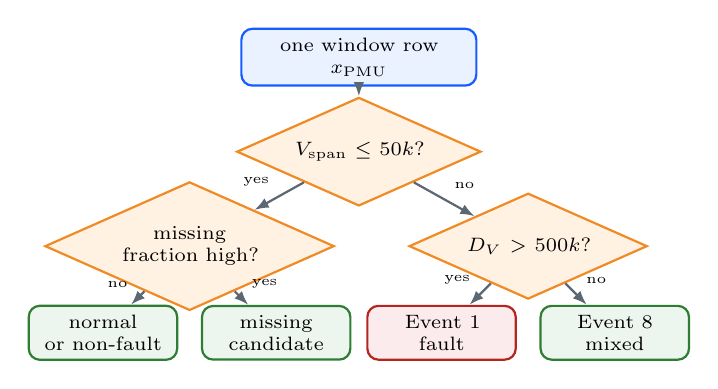
\begin{tikzpicture}[
  node distance=0.42cm,
  feat/.style={rounded corners=4pt,draw=Blue,fill=SoftBlue,thick,text width=2.75cm,minimum height=0.58cm,align=center,font=\scriptsize},
  test/.style={diamond,aspect=2.25,draw=Orange,fill=SoftOrange,thick,text width=1.8cm,align=center,font=\scriptsize},
  leaf/.style={rounded corners=4pt,draw=Green,fill=SoftGreen,thick,text width=1.65cm,minimum height=0.52cm,align=center,font=\scriptsize},
  leafr/.style={rounded corners=4pt,draw=Red,fill=SoftRed,thick,text width=1.65cm,minimum height=0.52cm,align=center,font=\scriptsize},
  arrow/.style={-{Latex[length=1.8mm]},thick,draw=Muted}
]
\node[feat] (row) at (0,2.45) {one window row\\$x_{\mathrm{PMU}}$};
\node[test] (root) at (0,1.25) {$V_{\mathrm{span}}\le 50k$?};
\node[test] (left) at (-2.15,0.05) {missing\\fraction high?};
\node[test] (right) at (2.15,0.05) {$D_V>500k$?};
\node[leaf] (normal) at (-3.25,-1.05) {normal\\or non-fault};
\node[leaf] (miss) at (-1.05,-1.05) {missing\\candidate};
\node[leafr] (fault) at (1.05,-1.05) {Event 1\\fault};
\node[leaf] (mixed) at (3.25,-1.05) {Event 8\\mixed};
\draw[arrow] (row) -- (root);
\draw[arrow] (root) -- node[above left,font=\tiny]{yes} (left);
\draw[arrow] (root) -- node[above right,font=\tiny]{no} (right);
\draw[arrow] (left) -- node[above left,font=\tiny]{no} (normal);
\draw[arrow] (left) -- node[above right,font=\tiny]{yes} (miss);
\draw[arrow] (right) -- node[above left,font=\tiny]{yes} (fault);
\draw[arrow] (right) -- node[above right,font=\tiny]{no} (mixed);
\end{tikzpicture}
}
\end{column}
\begin{column}{0.46\textwidth}
\centering
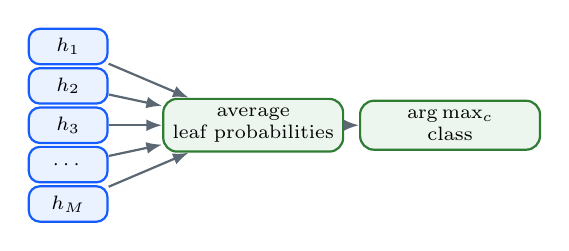
\begin{tikzpicture}[
  tree/.style={rounded corners=4pt,draw=Blue,fill=SoftBlue,thick,minimum width=1.0cm,minimum height=0.45cm,font=\scriptsize},
  vote/.style={rounded corners=5pt,draw=Green,fill=SoftGreen,thick,text width=2.05cm,minimum height=0.60cm,align=center,font=\scriptsize},
  arrow/.style={-{Latex[length=2mm]},thick,draw=Muted}
]
\node[tree] (t1) at (0,1.0) {$h_1$};
\node[tree] (t2) at (0,0.5) {$h_2$};
\node[tree] (t3) at (0,0.0) {$h_3$};
\node[tree] (t4) at (0,-0.5) {$\cdots$};
\node[tree] (t5) at (0,-1.0) {$h_M$};
\node[vote] (v) at (2.35,0) {average\\leaf probabilities};
\node[vote] (o) at (4.85,0) {$\arg\max_c$\\class};
\foreach \t in {t1,t2,t3,t4,t5} {
  \draw[arrow] (\t) -- (v);
}
\draw[arrow] (v) -- (o);
\end{tikzpicture}
\begin{block}{Forest probability}
\[
p_m(c\mid x)=\frac{n_{\mathrm{leaf},c}}{n_{\mathrm{leaf}}},
\qquad
\hat p(c\mid x)=\frac{1}{M}\sum_m p_m(c\mid x)
\]
\[
\hat c=\arg\max_c \hat p(c\mid x)
\]
\end{block}
\end{column}
\end{columns}
\vspace{-1mm}
\centering
{\footnotesize One tree follows a threshold path; ExtraTrees averages many randomized trees, so the submitted decision is a probability vote, not one manual rule.}
\end{frame}

% -------------------------------------------------------------------
\begin{frame}{Where ExtraTrees models are used and trained}
\scriptsize
\centering
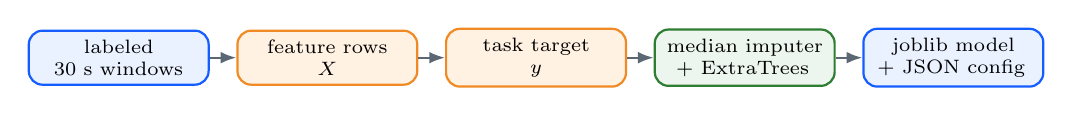
\begin{tikzpicture}[
  box/.style={rounded corners=5pt,draw=Blue,fill=SoftBlue,thick,text width=2.05cm,minimum height=0.58cm,align=center,font=\scriptsize},
  box2/.style={rounded corners=5pt,draw=Orange,fill=SoftOrange,thick,text width=2.05cm,minimum height=0.58cm,align=center,font=\scriptsize},
  box3/.style={rounded corners=5pt,draw=Green,fill=SoftGreen,thick,text width=2.05cm,minimum height=0.58cm,align=center,font=\scriptsize},
  arrow/.style={-{Latex[length=2mm]},thick,draw=Muted}
]
\node[box] (w) at (0,0) {labeled\\30 s windows};
\node[box2] (x) at (2.65,0) {feature rows\\$X$};
\node[box2] (y) at (5.30,0) {task target\\$y$};
\node[box3] (fit) at (7.95,0) {median imputer\\+ ExtraTrees};
\node[box] (job) at (10.60,0) {joblib model\\+ JSON config};
\draw[arrow] (w) -- (x);
\draw[arrow] (x) -- (y);
\draw[arrow] (y) -- (fit);
\draw[arrow] (fit) -- (job);
\end{tikzpicture}
\vspace{2mm}
\begin{tabular}{p{0.22\textwidth}p{0.31\textwidth}p{0.34\textwidth}}
\toprule
\textbf{ExtraTrees model} & \textbf{Training target} & \textbf{Inference role}\\
\midrule
Physical event classifier &
\code{physical\_event\_label}: 0,1,2,3,4,8 &
Main physical event evidence and confidence.\\
Bad-data detector &
Event 7 indicator / bad-data label &
Produces bad-data score for the rule engine.\\
Missing detector &
Missing-composition label &
Separates missing-only from missing + physical.\\
Typed localizers &
\code{location\_label} after filtering by \code{location\_type} and event &
Predicts BUS, LINE, or PMU origin after routing.\\
\bottomrule
\end{tabular}
\vspace{2mm}
\begin{columns}[T,totalwidth=\textwidth]
\begin{column}{0.48\textwidth}
\begin{block}{Training pattern}
\[
\texttt{model.fit}(X_{\mathrm{train}}, y_{\mathrm{task}})
\]
One supervised model per decision, using the same engineered feature rows but different labels.
\end{block}
\end{column}
\begin{column}{0.48\textwidth}
\begin{exampleblock}{Submitted runtime}
RAW PMU files $\rightarrow$ features $\rightarrow$ ExtraTrees scores $\rightarrow$ rule engine $\rightarrow$ typed localizer $\rightarrow$ CSV.
\end{exampleblock}
\end{column}
\end{columns}
\end{frame}

% -------------------------------------------------------------------
\begin{frame}{Hierarchical event routing}
\small
\centering
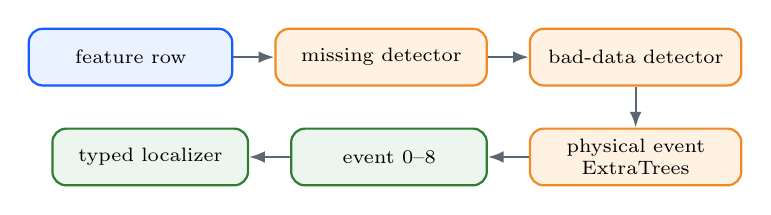
\begin{tikzpicture}[
  node distance=0.52cm,
  box/.style={rounded corners=5pt,draw=Blue,fill=SoftBlue,thick,text width=2.35cm,minimum height=0.72cm,align=center,font=\scriptsize},
  gate/.style={rounded corners=5pt,draw=Orange,fill=SoftOrange,thick,text width=2.45cm,minimum height=0.72cm,align=center,font=\scriptsize},
  outbox/.style={rounded corners=5pt,draw=Green,fill=SoftGreen,thick,text width=2.25cm,minimum height=0.72cm,align=center,font=\scriptsize},
  arrow/.style={-{Latex[length=2mm]},thick,draw=Muted}
]
\node[box] (x) {feature row};
\node[gate,right=of x] (miss) {missing detector};
\node[gate,right=of miss] (bad) {bad-data detector};
\node[gate,below=of bad] (phys) {physical event ExtraTrees};
\node[outbox,left=of phys] (event) {event 0--8};
\node[outbox,left=of event] (loc) {typed localizer};
\draw[arrow] (x) -- (miss);
\draw[arrow] (miss) -- (bad);
\draw[arrow] (bad) -- (phys);
\draw[arrow] (phys) -- (event);
\draw[arrow] (event) -- (loc);
\end{tikzpicture}
\vspace{2mm}
\begin{block}{Decision order}
Missing and bad-data evidence is routed before the physical classifier so communication failures and sensor artifacts do not contaminate physical events.
\end{block}
\end{frame}

% -------------------------------------------------------------------
\begin{frame}{Physics rule guards and tree decision}
\scriptsize
\begin{columns}[T,totalwidth=\textwidth]
\begin{column}{0.48\textwidth}
\begin{alertblock}{Main guards}
\[
V_{\mathrm{span}}\ge50{,}000\ \lor\ D_V\ge500{,}000
\Rightarrow \mathrm{fault\ candidate}
\]
\[
I_{\mathrm{span}}\ge500,\quad D_I\ge3{,}000,\quad V_{\mathrm{span}}\le50{,}000
\]
\[
\Rightarrow \mathrm{line\ outage\ candidate}
\]
\[
\mathrm{single\_signal\_score}\ge200{,}000,\quad
\mathrm{ratio}\ge3
\Rightarrow \mathrm{bad\ data}
\]
\end{alertblock}
\end{column}
\begin{column}{0.48\textwidth}
\begin{block}{Tree role}
ExtraTrees estimates class probabilities from the full engineered vector. Rule guards override only high-risk confusion points: missing, bad data, fault, and line outage.
\end{block}
\begin{exampleblock}{Output}
\[
\hat{e}=\arg\max_e p(e\mid x),\qquad
\hat{\ell}=\arg\max_\ell p(\ell\mid x,\hat{e})
\]
\end{exampleblock}
\end{column}
\end{columns}
\end{frame}

\iffalse
\begin{frame}{Hierarchical event logic}
\centering
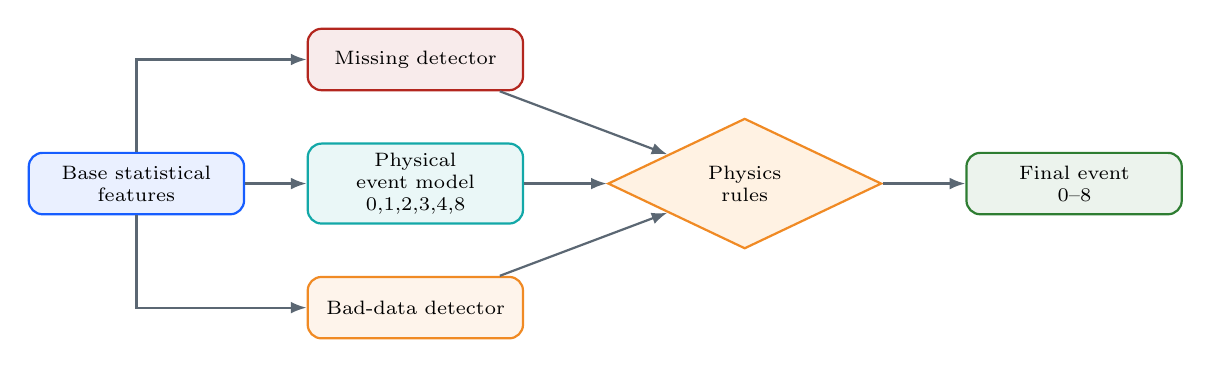
\begin{tikzpicture}[
  node distance=0.65cm and 0.78cm,
  boxblue/.style={rounded corners=5pt,draw=Blue,fill=Blue!9,thick,text width=2.5cm,minimum height=0.78cm,align=center,font=\scriptsize},
  boxcyan/.style={rounded corners=5pt,draw=Cyan,fill=Cyan!9,thick,text width=2.5cm,minimum height=0.78cm,align=center,font=\scriptsize},
  boxgreen/.style={rounded corners=5pt,draw=Green,fill=Green!9,thick,text width=2.5cm,minimum height=0.78cm,align=center,font=\scriptsize},
  boxorange/.style={rounded corners=5pt,draw=Orange,fill=Orange!9,thick,text width=2.5cm,minimum height=0.78cm,align=center,font=\scriptsize},
  boxred/.style={rounded corners=5pt,draw=Red,fill=Red!9,thick,text width=2.5cm,minimum height=0.78cm,align=center,font=\scriptsize},
  gate/.style={diamond,aspect=2.1,draw=Orange,fill=SoftOrange,thick,text width=1.8cm,align=center,font=\scriptsize},
  arrow/.style={-{Latex[length=2mm]},thick,draw=Muted}
]
\node[boxblue] (x) {Base statistical\\features};
\node[boxcyan,right=of x] (phys) {Physical event model\\0,1,2,3,4,8};
\node[boxred,above=of phys] (miss) {Missing detector};
\node[boxorange,below=of phys] (bad) {Bad-data detector};
\node[gate,right=1.05cm of phys] (rules) {Physics\\rules};
\node[boxgreen,right=1.05cm of rules] (event) {Final event\\0--8};
\draw[arrow] (x) -- (phys);
\draw[arrow] (x) |- (miss);
\draw[arrow] (x) |- (bad);
\draw[arrow] (phys) -- (rules);
\draw[arrow] (miss) -- (rules);
\draw[arrow] (bad) -- (rules);
\draw[arrow] (rules) -- (event);
\end{tikzpicture}
\vspace{4mm}
\begin{block}{Hierarchical routing rationale}
Missing data and bad data are measurement phenomena. They should not be forced into the same flat classifier decision as physical grid events.
\end{block}
\end{frame}

% -------------------------------------------------------------------
\begin{frame}{Physics rule guards}
\small
\begin{columns}[T,totalwidth=\textwidth]
\begin{column}{0.50\textwidth}
\begin{block}{Fault-like}
\[
V_{\mathrm{span}} \ge 50{,}000
\quad\mathrm{or}\quad
\max |dV/dt| \ge 500{,}000
\]
\end{block}
\begin{block}{Line-outage-like}
\[
I_{\mathrm{span}} \ge 500
\]
\[
\max |dI/dt| \ge 3{,}000
\]
\[
V_{\mathrm{span}} \le 50{,}000
\]
\end{block}
\end{column}
\begin{column}{0.46\textwidth}
\begin{alertblock}{Missing-like}
\[
\mathrm{data\_present\_fraction}<0.999
\]
or high NaN/gap features.
\end{alertblock}
\begin{alertblock}{Bad-data-like}
\[
\mathrm{single\_signal\_score}\ge 200{,}000
\]
\[
\mathrm{single\_signal\_ratio}\ge 3.0
\]
\end{alertblock}
\end{column}
\end{columns}
\end{frame}

% -------------------------------------------------------------------
\begin{frame}{Rule engine as a decision tree}
\small
\centering
\resizebox{!}{0.48\textheight}{%
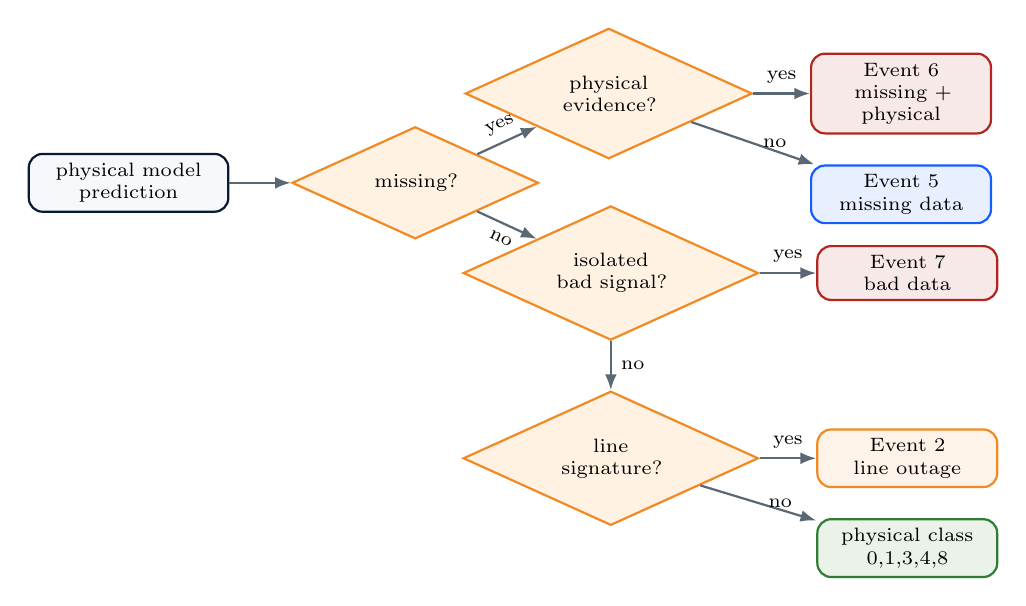
\begin{tikzpicture}[
  node distance=0.55cm and 0.78cm,
  decision/.style={diamond,aspect=2.2,draw=Orange,fill=SoftOrange,thick,text width=1.9cm,align=center,font=\scriptsize},
  leafred/.style={rounded corners=5pt,draw=Red,fill=Red!10,thick,text width=2.05cm,minimum height=0.68cm,align=center,font=\scriptsize},
  leafblue/.style={rounded corners=5pt,draw=Blue,fill=Blue!10,thick,text width=2.05cm,minimum height=0.68cm,align=center,font=\scriptsize},
  leaforange/.style={rounded corners=5pt,draw=Orange,fill=Orange!10,thick,text width=2.05cm,minimum height=0.68cm,align=center,font=\scriptsize},
  leafgreen/.style={rounded corners=5pt,draw=Green,fill=Green!10,thick,text width=2.05cm,minimum height=0.68cm,align=center,font=\scriptsize},
  proc/.style={rounded corners=5pt,draw=Navy,fill=Paper,thick,text width=2.3cm,minimum height=0.68cm,align=center,font=\scriptsize},
  arrow/.style={-{Latex[length=2mm]},thick,draw=Muted}
]
\node[proc] (phys) {physical model\\prediction};
\node[decision,right=of phys] (miss) {missing?};
\node[decision,above right=0.35cm and 0.75cm of miss] (physe) {physical\\evidence?};
\node[leafred,right=0.72cm of physe] (e6) {Event 6\\missing + physical};
\node[leafblue,below=0.38cm of e6] (e5) {Event 5\\missing data};
\node[decision,below right=0.35cm and 0.75cm of miss] (bad) {isolated\\bad signal?};
\node[leafred,right=0.72cm of bad] (e7) {Event 7\\bad data};
\node[decision,below=0.62cm of bad] (line) {line\\signature?};
\node[leaforange,right=0.72cm of line] (e2) {Event 2\\line outage};
\node[leafgreen,below=0.38cm of e2] (physout) {physical class\\0,1,3,4,8};
\draw[arrow] (phys) -- (miss);
\draw[arrow] (miss) -- node[above,sloped]{\scriptsize yes} (physe);
\draw[arrow] (physe) -- node[above]{\scriptsize yes} (e6);
\draw[arrow] (physe) -- node[right]{\scriptsize no} (e5);
\draw[arrow] (miss) -- node[below,sloped]{\scriptsize no} (bad);
\draw[arrow] (bad) -- node[above]{\scriptsize yes} (e7);
\draw[arrow] (bad) -- node[right]{\scriptsize no} (line);
\draw[arrow] (line) -- node[above]{\scriptsize yes} (e2);
\draw[arrow] (line) -- node[right]{\scriptsize no} (physout);
\end{tikzpicture}%
}
\vspace{0.5mm}
\begin{block}{Additional implementation gates}
The implementation also uses confidence gates so weak physical predictions do not override strong missing or bad-data evidence.
\end{block}
\end{frame}

% -------------------------------------------------------------------

% -------------------------------------------------------------------
\fi
\section{Event-by-Event Interpretation}
\sectionframe{}{Event-by-Event\\Interpretation}{How each event type is recognized}


% -------------------------------------------------------------------
\begin{frame}{Event 1: fault}
\small
\begin{columns}[T,totalwidth=\textwidth]
\begin{column}{0.48\textwidth}
\begin{block}{Main evidence}
\begin{itemize}
  \item Voltage magnitude span.
  \item Voltage derivative.
  \item Robust z-score in voltage channels.
  \item Early segment changes.
  \item Cross-PMU severity pattern.
\end{itemize}
\end{block}
\end{column}
\begin{column}{0.48\textwidth}
\begin{alertblock}{Manual recipe}
\begin{enumerate}
  \item Build baseline from pre-event voltage.
  \item Detect large voltage sag/transient.
  \item Reject missing-only and bad-data-only cases.
  \item Localize to BUS using spatial severity.
\end{enumerate}
\end{alertblock}
\end{column}
\end{columns}
\end{frame}

% -------------------------------------------------------------------
\begin{frame}{Event 2: line outage}
\small
\begin{columns}[T,totalwidth=\textwidth]
\begin{column}{0.48\textwidth}
\begin{block}{Main evidence}
\begin{itemize}
  \item Current magnitude span.
  \item Current derivative.
  \item Current-angle changes.
  \item Voltage span not as extreme as a fault.
  \item Graph-temporal pairwise PMU differences.
\end{itemize}
\end{block}
\end{column}
\begin{column}{0.48\textwidth}
\begin{alertblock}{Manual recipe}
\begin{enumerate}
  \item Look for current redistribution.
  \item Guard against fault-like voltage collapse.
  \item Use graph features to score candidate lines.
  \item Localize to LINE.
\end{enumerate}
\end{alertblock}
\end{column}
\end{columns}
\end{frame}

% -------------------------------------------------------------------

% -------------------------------------------------------------------

% -------------------------------------------------------------------

% -------------------------------------------------------------------
\begin{frame}{Event 7: bad data}
\small
\begin{columns}[T,totalwidth=\textwidth]
\begin{column}{0.48\textwidth}
\begin{block}{Main evidence}
\begin{itemize}
  \item One signal has extreme robust z-score.
  \item Top anomaly is much larger than second anomaly.
  \item Other PMUs/channels remain coherent.
  \item Missing features do not dominate.
\end{itemize}
\end{block}
\end{column}
\begin{column}{0.48\textwidth}
\begin{alertblock}{Localizer}
Event 7 localizes to PMU, not BUS or LINE. The object that failed is the measurement device/channel source.
\end{alertblock}
\end{column}
\end{columns}
\end{frame}

% -------------------------------------------------------------------
\begin{frame}{Event 8: unknown physical proxy}
\small
\begin{block}{Main evidence}
Event 8 captures cases with physical evidence that does not cleanly fit fault, line outage, generation change, or load change.
\end{block}
\begin{columns}[T,totalwidth=\textwidth]
\begin{column}{0.48\textwidth}
\begin{exampleblock}{Useful features}
\begin{itemize}
  \item Power proxy.
  \item Rolling dynamics.
  \item Adaptive residual and innovation features.
  \item Graph-temporal pattern.
\end{itemize}
\end{exampleblock}
\end{column}
\begin{column}{0.48\textwidth}
\begin{alertblock}{Routing}
The final runtime routes Event 8 to a BUS localizer because it represents a physical-grid signature rather than a PMU-only failure.
\end{alertblock}
\end{column}
\end{columns}
\end{frame}

% -------------------------------------------------------------------
\section{Localization}
\sectionframe{}{Localization}{Typed localizers and the hybrid bus estimate}


% -------------------------------------------------------------------
\begin{frame}{Typed origin localization}
\scriptsize
\begin{columns}[T,totalwidth=\textwidth]
\begin{column}{0.48\textwidth}
\begin{block}{Route before predicting origin}
\begin{tabular}{@{}cl@{}}
\toprule
Predicted event & Candidate origin set\\
\midrule
0 normal & NONE\\
1 fault & BUS labels\\
2 line outage & LINE labels\\
3 generation change & BUS labels\\
4 load change & BUS labels\\
5 missing data & PMU labels\\
6 missing + physical & physical route\\
7 bad data & PMU labels\\
8 mixed physical proxy & BUS labels\\
\bottomrule
\end{tabular}
\end{block}
\vspace{1mm}
\tiny
For event 6: \(\hat e_{\mathrm{phys}}=2\Rightarrow\) LINE; otherwise BUS.
\end{column}
\begin{column}{0.48\textwidth}
\begin{alertblock}{Implemented decision}
The model does not rank every possible label together. It first chooses a type, then runs the localizer trained for that type.
\end{alertblock}
\centering
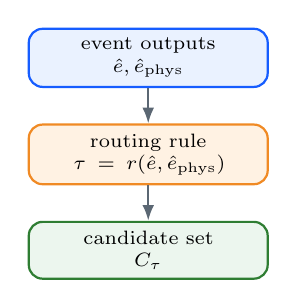
\begin{tikzpicture}[
  node distance=0.45cm,
  box/.style={rounded corners=5pt,draw=Blue,fill=SoftBlue,thick,text width=2.8cm,minimum height=0.66cm,align=center,font=\scriptsize},
  box2/.style={rounded corners=5pt,draw=Orange,fill=SoftOrange,thick,text width=2.8cm,minimum height=0.66cm,align=center,font=\scriptsize},
  box3/.style={rounded corners=5pt,draw=Green,fill=SoftGreen,thick,text width=2.8cm,minimum height=0.66cm,align=center,font=\scriptsize},
  arrow/.style={-{Latex[length=2mm]},thick,draw=Muted}
]
\node[box] (evt) {event outputs\\$\hat e,\hat e_{\rm phys}$};
\node[box2,below=of evt] (route) {routing rule\\$\tau=r(\hat e,\hat e_{\rm phys})$};
\node[box3,below=of route] (cands) {candidate set\\$C_\tau$};
\draw[arrow] (evt) -- (route);
\draw[arrow] (route) -- (cands);
\end{tikzpicture}
\end{column}
\end{columns}
\end{frame}

% -------------------------------------------------------------------
\begin{frame}{Three origin spaces}
\small
\centering
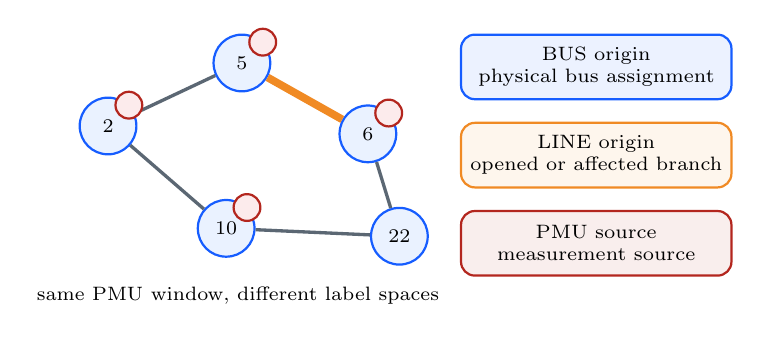
\begin{tikzpicture}[
  bus/.style={circle,draw=Blue,fill=SoftBlue,thick,minimum size=0.72cm,font=\scriptsize},
  pmu/.style={circle,draw=Red,fill=SoftRed,thick,minimum size=0.34cm},
  line/.style={draw=Muted,line width=1.2pt},
  label/.style={font=\scriptsize,align=center},
  boxblue/.style={rounded corners=5pt,draw=Blue,fill=Blue!8,thick,text width=3.2cm,minimum height=0.82cm,align=center,font=\scriptsize},
  boxorange/.style={rounded corners=5pt,draw=Orange,fill=Orange!8,thick,text width=3.2cm,minimum height=0.82cm,align=center,font=\scriptsize},
  boxred/.style={rounded corners=5pt,draw=Red,fill=Red!8,thick,text width=3.2cm,minimum height=0.82cm,align=center,font=\scriptsize}
]
\node[bus] (b2) at (0,1.4) {2};
\node[bus] (b5) at (1.7,2.2) {5};
\node[bus] (b6) at (3.3,1.3) {6};
\node[bus] (b10) at (1.5,0.1) {10};
\node[bus] (b22) at (3.7,0.0) {22};
\draw[line] (b2) -- (b5);
\draw[line,Orange,line width=2.8pt] (b5) -- (b6);
\draw[line] (b2) -- (b10);
\draw[line] (b10) -- (b22);
\draw[line] (b6) -- (b22);
\node[pmu] at (b2.north east) {};
\node[pmu] at (b5.north east) {};
\node[pmu] at (b6.north east) {};
\node[pmu] at (b10.north east) {};
\node[boxblue] at (6.2,2.15) {BUS origin\\physical bus assignment};
\node[boxorange] at (6.2,1.03) {LINE origin\\opened or affected branch};
\node[boxred] at (6.2,-0.09) {PMU source\\measurement source};
\node[label] at (1.65,-0.75) {same PMU window, different label spaces};
\end{tikzpicture}
\vspace{2mm}
\begin{block}{Location semantics}
\code{pred\_location} is typed. A label such as \code{5} can mean bus 5 in BUS mode, while PMU mode means the PMU/source indexed by 5.
\end{block}
\end{frame}

% -------------------------------------------------------------------
\begin{frame}{Final localizer models}
\small
\begin{block}{Model lookup used at inference}
\centering
\begin{tabular}{@{}ll@{}}
\toprule
First choice & Fallback\\
\midrule
\code{BUS:event1}, \code{BUS:event3}, \code{BUS:event4}, \code{BUS:event8} & \code{BUS}\\
\code{LINE:event2} & \code{LINE}\\
\code{PMU} & \code{PMU}\\
\bottomrule
\end{tabular}
\end{block}
\begin{exampleblock}{Model family}
Each entry is a median-imputed ExtraTrees pipeline trained on the localizer feature vector. Event-specific models are used when the physical event prediction selects one.
\end{exampleblock}
\begin{alertblock}{Final Top-1}
\code{use\_hybrid\_top1 = false}. The final submitted Top-1 location uses the validated typed ML localizers, not the hybrid/oracle branch.
\end{alertblock}
\end{frame}

% -------------------------------------------------------------------
\begin{frame}{Localizer evidence and inference equation}
\small
\begin{columns}[T,totalwidth=\textwidth]
\begin{column}{0.48\textwidth}
\begin{block}{Evidence used}
\begin{itemize}
  \item local PMU amplitude and robust z-score;
  \item derivative and residual/innovation peak timing;
  \item graph-temporal pair differences and electrical-distance weights;
  \item event-specific candidate space: BUS, LINE, or PMU.
\end{itemize}
\end{block}
\end{column}
\begin{column}{0.48\textwidth}
\begin{alertblock}{Inference}
\[
p_\tau(\ell\mid x)=\frac{1}{T}\sum_{m=1}^{T}
\mathbf{1}\{h_m(x)=\ell\}
\]
\[
\hat{\ell}=\arg\max_{\ell\in\mathcal{L}_\tau}p_\tau(\ell\mid x)
\]
\end{alertblock}
\begin{exampleblock}{Interpretation}
The event route selects the localizer type \(\tau\), then the ExtraTrees model ranks candidates only inside \(\mathcal{L}_\tau\).
\end{exampleblock}
\end{column}
\end{columns}
\end{frame}

% -------------------------------------------------------------------
\begin{frame}{Localizer target spaces and error sources}
\small
\begin{columns}[T,totalwidth=\textwidth]
\begin{column}{0.48\textwidth}
\begin{block}{Candidate spaces}
\begin{tabular}{ll}
\toprule
Route & Candidates\\
\midrule
BUS & IEEE 39 buses\\
LINE & branch candidates\\
PMU & observed PMUs / failed channels\\
\bottomrule
\end{tabular}
\end{block}
\begin{alertblock}{Typed routing}
BUS, LINE, and PMU labels are never mixed in one flat label space.
\end{alertblock}
\end{column}
\begin{column}{0.48\textwidth}
\begin{exampleblock}{Main error sources}
Sparse PMU coverage, electrically close candidates, topology-dependent fingerprints, and event types with similar voltage/current signatures.
\end{exampleblock}
\begin{block}{Practical effect}
Classification is easier than localization; localization must infer an unobserved origin from a few observed PMU responses.
\end{block}
\end{column}
\end{columns}
\end{frame}

\iffalse
\begin{frame}{Localizer feature evidence}
\small
\begin{columns}[T,totalwidth=\textwidth]
\begin{column}{0.32\textwidth}
\begin{block}{BUS}
\begin{itemize}
  \item strongest voltage or frequency deviation,
  \item earliest residual/innovation,
  \item graph spread across nearby PMUs.
\end{itemize}
\end{block}
\end{column}
\begin{column}{0.32\textwidth}
\begin{block}{LINE}
\begin{itemize}
  \item current redistribution after opening,
  \item pair differences across candidate branch,
  \item topology-weighted response asymmetry.
\end{itemize}
\end{block}
\end{column}
\begin{column}{0.32\textwidth}
\begin{block}{PMU}
\begin{itemize}
  \item missing run length,
  \item isolated channel abnormality,
  \item source-local NaN or bad-data score.
\end{itemize}
\end{block}
\end{column}
\end{columns}
\vspace{2mm}
\begin{alertblock}{Location signal}
The localizer uses spatial contrast: which PMU changed, when it changed, and how that pattern matches the grid topology.
\end{alertblock}
\end{frame}

% -------------------------------------------------------------------
\begin{frame}{Localizer inference equation}
\small
\begin{columns}[T,totalwidth=\textwidth]
\begin{column}{0.52\textwidth}
\begin{block}{Typed classification}
\[
x_{\mathrm{loc}}=
\left[
x_{\mathrm{base}},\
x_{\mathrm{rolling}},\
x_{\mathrm{residual}},\
x_{\mathrm{graph}}
\right]
\]
\[
\tau=r(\hat e,\hat e_{\mathrm{phys}})
\]
\[
C_\tau\in\{\mathcal Y_{BUS},\mathcal Y_{LINE},\mathcal Y_{PMU}\}
\]
\[
\hat{\ell}=
\arg\max_{\ell\in C_\tau}
p_{\mathrm{ET},\tau}(\ell\mid x_{\mathrm{loc}})
\]
\end{block}
\begin{exampleblock}{Meaning}
The classifier only compares labels inside the selected origin space.
\end{exampleblock}
\end{column}
\begin{column}{0.44\textwidth}
\centering
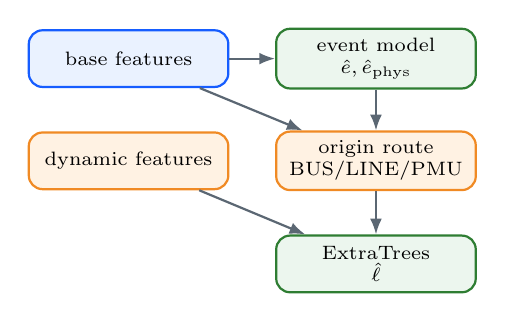
\begin{tikzpicture}[
  node distance=0.55cm,
  box/.style={rounded corners=5pt,draw=Blue,fill=SoftBlue,thick,text width=2.30cm,minimum height=0.72cm,align=center,font=\scriptsize},
  box2/.style={rounded corners=5pt,draw=Orange,fill=SoftOrange,thick,text width=2.30cm,minimum height=0.72cm,align=center,font=\scriptsize},
  box3/.style={rounded corners=5pt,draw=Green,fill=SoftGreen,thick,text width=2.30cm,minimum height=0.72cm,align=center,font=\scriptsize},
  arrow/.style={-{Latex[length=2mm]},thick,draw=Muted}
]
\node[box] (base) {base features};
\node[box2,below=of base] (dyn) {dynamic features};
\node[box3,right=0.58cm of base] (event) {event model\\$\hat e,\hat e_{\rm phys}$};
\node[box2,right=0.58cm of dyn] (route) {origin route\\BUS/LINE/PMU};
\node[box3,below=of route] (loc) {ExtraTrees\\$\hat{\ell}$};
\draw[arrow] (base) -- (event);
\draw[arrow] (event) -- (route);
\draw[arrow] (base) -- (route);
\draw[arrow] (route) -- (loc);
\draw[arrow] (dyn) -- (loc);
\end{tikzpicture}
\vspace{2mm}
\begin{alertblock}{Reason for two feature views}
The event classifier uses the stable base vector. The localizer also uses dynamic propagation and topology features.
\end{alertblock}
\end{column}
\end{columns}
\end{frame}

% -------------------------------------------------------------------
\begin{frame}{BUS, LINE, and PMU targets}
\small
\begin{columns}[T,totalwidth=\textwidth]
\begin{column}{0.32\textwidth}
\begin{block}{BUS}
\[
\mathcal{Y}_{BUS}=\{1,\dots,39\}
\]
Target is the electrical bus where the physical disturbance is assigned.
\end{block}
\end{column}
\begin{column}{0.32\textwidth}
\begin{block}{LINE}
\[
\mathcal{Y}_{LINE}=\{(i,j):(i,j)\in\mathcal{E}\}
\]
Target is a branch in the IEEE 39 topology.
\end{block}
\end{column}
\begin{column}{0.32\textwidth}
\begin{block}{PMU}
\[
\begin{gathered}
\mathcal{Y}_{PMU}=\\
\{2,5,6,10,19,22,29,39\}
\end{gathered}
\]
Target is the observed source affected by missing or bad data.
\end{block}
\end{column}
\end{columns}
\vspace{2mm}
\centering
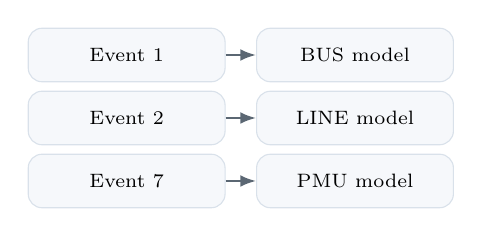
\begin{tikzpicture}[
  target/.style={rounded corners=5pt,draw=Line,fill=Paper,minimum width=2.5cm,minimum height=0.68cm,align=center,font=\scriptsize},
  arrow/.style={-{Latex[length=2mm]},thick,draw=Muted}
]
\node[target] (e1) at (0,0) {Event 1};
\node[target] (bus) at (2.9,0) {BUS model};
\node[target] (e2) at (0,-0.8) {Event 2};
\node[target] (line) at (2.9,-0.8) {LINE model};
\node[target] (e7) at (0,-1.6) {Event 7};
\node[target] (pmu) at (2.9,-1.6) {PMU model};
\draw[arrow] (e1) -- (bus);
\draw[arrow] (e2) -- (line);
\draw[arrow] (e7) -- (pmu);
\end{tikzpicture}
\end{frame}

% -------------------------------------------------------------------
\begin{frame}{Localization error sources}
\small
\begin{columns}[T,totalwidth=\textwidth]
\begin{column}{0.55\textwidth}
\centering
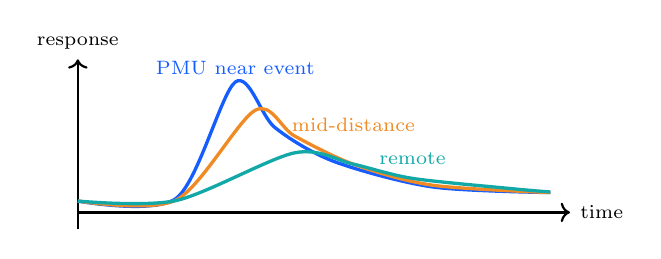
\begin{tikzpicture}[x=0.25cm,y=0.72cm]
  \draw[->,thick] (0,0) -- (25,0) node[right]{\scriptsize time};
  \draw[->,thick] (0,-0.3) -- (0,2.7) node[above]{\scriptsize response};
  \draw[Blue,very thick,smooth] plot coordinates {(0,0.2)(5,0.25)(8,2.3)(10,1.5)(13,0.9)(18,0.45)(24,0.35)};
  \draw[Orange,very thick,smooth] plot coordinates {(0,0.2)(5,0.22)(9,1.8)(11,1.35)(14,0.85)(18,0.48)(24,0.35)};
  \draw[Cyan,very thick,smooth] plot coordinates {(0,0.2)(5,0.21)(11,1.05)(14,0.85)(17,0.60)(22,0.42)(24,0.36)};
  \node[Blue] at (8,2.55) {\scriptsize PMU near event};
  \node[Orange] at (14,1.55) {\scriptsize mid-distance};
  \node[Cyan] at (17,0.95) {\scriptsize remote};
\end{tikzpicture}
\end{column}
\begin{column}{0.41\textwidth}
\begin{block}{Classification}
Often needs to know whether the pattern resembles a fault, outage, load change, missing data, or bad data.
\end{block}
\begin{alertblock}{Localization}
Needs spatial ordering: which PMU changed first, which changed most, and which candidate explains the pattern.
\end{alertblock}
\end{column}
\end{columns}
\end{frame}

% -------------------------------------------------------------------
\fi
\section{Training, Validation, and Results}
\sectionframe{}{Training, Validation,\\and Results}{Evaluation protocol and reported metrics}


% -------------------------------------------------------------------
\begin{frame}{Training data and split}
\small
\begin{columns}[T,totalwidth=\textwidth]
\begin{column}{0.48\textwidth}
\begin{block}{Training sources}
\begin{itemize}
  \item 5,000 synthetic SGSMA scenario windows.
  \item 3,500 train windows and 1,500 stratified holdout windows.
  \item Base statistical and dynamic tables generated by the repo feature extractors.
  \item Random state: \code{20260503}.
\end{itemize}
\end{block}
\end{column}
\begin{column}{0.48\textwidth}
\begin{exampleblock}{Validation}
\begin{itemize}
  \item 30\% stratified SIM holdout.
  \item RAW0001 transfer validation.
  \item Metrics: detector, classifier, macro-F1, localization.
\end{itemize}
\end{exampleblock}
\end{column}
\end{columns}
\vspace{2mm}
\begin{alertblock}{Transfer principle}
RAW labels were used for validation and analysis, not to train the final production-feasible submission path.
\end{alertblock}
\end{frame}

% -------------------------------------------------------------------
\begin{frame}{Final metrics}
\small
\begin{columns}[T,totalwidth=\textwidth]
\begin{column}{0.49\textwidth}
\begin{block}{SIM holdout}
\centering
\begin{tabular}{lr}
\toprule
Metric & Score\\
\midrule
Detector accuracy & 0.9693\\
Classifier accuracy & 0.9673\\
Classifier macro-F1 & 0.9598\\
Localizer Top-1 & 0.8524\\
\bottomrule
\end{tabular}
\end{block}
\end{column}
\begin{column}{0.47\textwidth}
\begin{alertblock}{RAW0001}
\centering
\begin{tabular}{lr}
\toprule
Metric & Score\\
\midrule
Detector accuracy & 1.0000\\
Classifier accuracy & 1.0000\\
Classifier macro-F1 & 1.0000\\
Localizer Top-1 & 0.6667\\
\bottomrule
\end{tabular}
\end{alertblock}
\end{column}
\end{columns}
\vspace{2mm}
\begin{exampleblock}{Interpretation}
Detection and classification transferred perfectly on RAW0001; localization remained the hard part.
\end{exampleblock}
\end{frame}

% -------------------------------------------------------------------
\begin{frame}{Variant selection evidence}
\small
\begin{block}{Selected variant}
\[
\texttt{base statistical + rolling + adaptive residual + graph-temporal}
\]
\end{block}
\begin{columns}[T,totalwidth=\textwidth]
\begin{column}{0.48\textwidth}
\begin{exampleblock}{Selection evidence}
\begin{itemize}
  \item SIM detector accuracy: 0.9693.
  \item SIM classifier macro-F1: 0.9598.
  \item RAW0001 localization Top-1: 0.6667.
  \item No oracle RAW label use.
  \item No large NN/GNN training-data requirement.
\end{itemize}
\end{exampleblock}
\end{column}
\begin{column}{0.48\textwidth}
\begin{alertblock}{Tradeoff}
Some experimental methods had higher RAW0001 numbers, but were not valid for unseen data because they used RAW true labels or oracle assumptions.
\end{alertblock}
\end{column}
\end{columns}
\end{frame}

% -------------------------------------------------------------------
\begin{frame}{DeepSeek experiments in context}
\small
\begin{block}{DeepSeek role}
DeepSeek-assisted experiments tested RAW0001 behavior and candidate localization ideas. They were analysis runs, not the submitted inference route.
\end{block}
\begin{alertblock}{Excluded from inference}
Higher RAW0001 numbers came from variants that used RAW labels for training, oversampling, weighting, or oracle ranking. Those settings are invalid for a new hidden dataset.
\end{alertblock}
\begin{exampleblock}{Submitted method}
The final submitted method was SGMS: physics-informed features + hierarchical ExtraTrees + typed dynamic localizers.
\end{exampleblock}
\end{frame}

% -------------------------------------------------------------------
\section{Ablation and Reimplementation}
\sectionframe{}{Ablation and\\Reimplementation}{What each component contributes}


% -------------------------------------------------------------------
\begin{frame}{Implementation map and execution order}
\small
\begin{columns}[T,totalwidth=\textwidth]
\begin{column}{0.55\textwidth}
\centering
\resizebox{\linewidth}{!}{%
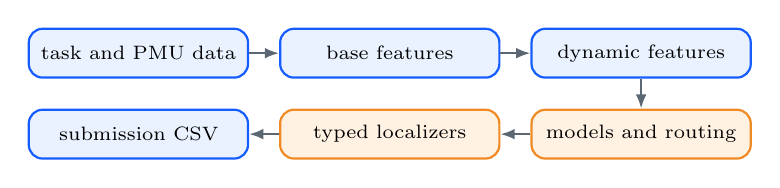
\begin{tikzpicture}[
  node distance=0.38cm,
  box/.style={rounded corners=5pt,draw=Blue,fill=SoftBlue,thick,text width=2.55cm,minimum height=0.62cm,align=center,font=\scriptsize},
  box2/.style={rounded corners=5pt,draw=Orange,fill=SoftOrange,thick,text width=2.55cm,minimum height=0.62cm,align=center,font=\scriptsize},
  arrow/.style={-{Latex[length=1.8mm]},thick,draw=Muted}
]
\node[box] (a) {task and PMU data};
\node[box,right=of a] (b) {base features};
\node[box,right=of b] (c) {dynamic features};
\node[box2,below=of c] (d) {models and routing};
\node[box2,left=of d] (e) {typed localizers};
\node[box,left=of e] (f) {submission CSV};
\draw[arrow] (a) -- (b);
\draw[arrow] (b) -- (c);
\draw[arrow] (c) -- (d);
\draw[arrow] (d) -- (e);
\draw[arrow] (e) -- (f);
\end{tikzpicture}}
\end{column}
\begin{column}{0.41\textwidth}
\begin{block}{Primary path}
Input windows, feature construction, event routing, and typed localization form the deployable method.
\end{block}
\begin{alertblock}{Implementation checks}
Equations, event recipes, thresholds, and validation commands are used as audit points while rebuilding.
\end{alertblock}
\end{column}
\end{columns}
\end{frame}

% -------------------------------------------------------------------
\begin{frame}{Ablation evidence}
\small
\begin{columns}[T,totalwidth=\textwidth]
\begin{column}{0.52\textwidth}
\centering
\begin{tikzpicture}[x=0.82cm,y=0.035cm]
  \draw[->,thick] (0,0) -- (5.7,0);
  \draw[->,thick] (0,0) -- (0,80) node[above]{\scriptsize Top-1};
  \foreach \y in {20,40,60} {\draw[Muted!40] (0,\y) -- (5.2,\y); \node[left] at (0,\y) {\scriptsize \y};}
  \fill[Blue!65] (0.45,0) rectangle (1.05,58);
  \fill[Cyan!65] (1.45,0) rectangle (2.05,64);
  \fill[Orange!75] (2.45,0) rectangle (3.05,67);
  \fill[Green!65] (3.45,0) rectangle (4.05,66.7);
  \node[rotate=45,anchor=east,font=\tiny] at (0.8,-4) {base};
  \node[rotate=45,anchor=east,font=\tiny] at (1.8,-4) {+rolling};
  \node[rotate=45,anchor=east,font=\tiny] at (2.8,-4) {+residual};
  \node[rotate=45,anchor=east,font=\tiny] at (3.8,-4) {final};
\end{tikzpicture}
\end{column}
\begin{column}{0.44\textwidth}
\begin{block}{Selection evidence}
The selected variant tied the best deployable RAW0001 localization result while keeping SIM validation strong.
\end{block}
\begin{alertblock}{Rejected variants}
RAW-label-trained, oracle, or leakage-dependent variants were not deployable on a new hidden RAW dataset.
\end{alertblock}
\end{column}
\end{columns}
\end{frame}

\iffalse
\begin{frame}{Evidence-to-implementation map}
\small
\begin{columns}[T,totalwidth=\textwidth]
\begin{column}{0.56\textwidth}
\centering
\begin{tikzpicture}[
  main/.style={rounded corners=5pt,draw=Blue,fill=SoftBlue,thick,text width=3.2cm,minimum height=0.75cm,align=center,font=\scriptsize},
  app/.style={rounded corners=5pt,draw=Orange,fill=SoftOrange,thick,text width=3.2cm,minimum height=0.75cm,align=center,font=\scriptsize},
  arrow/.style={-{Latex[length=2mm]},thick,draw=Muted}
]
\node[main] (a) at (0,1.8) {Inference path};
\node[main] (b) at (0,0.75) {Feature extraction};
\node[main] (c) at (0,-0.30) {Variant evidence};
\node[main] (d) at (0,-1.35) {Rebuild sequence};
\node[app] (e) at (4.5,1.25) {Audit checks};
\node[app] (f) at (4.5,0.20) {Equations, residuals,\\innovation, graph features};
\node[app] (g) at (4.5,-0.85) {Event recipes and\\failure modes};
\draw[arrow] (a) -- (b);
\draw[arrow] (b) -- (c);
\draw[arrow] (c) -- (d);
\draw[arrow] (a) -- (e);
\draw[arrow] (e) -- (f);
\draw[arrow] (f) -- (g);
\end{tikzpicture}
\end{column}
\begin{column}{0.40\textwidth}
\begin{block}{Primary path}
Input windows, feature construction, event routing, and typed localization form the deployable method.
\end{block}
\begin{alertblock}{Implementation checks}
Equations, event recipes, thresholds, and validation commands support implementation checks.
\end{alertblock}
\end{column}
\end{columns}
\end{frame}

% -------------------------------------------------------------------
\begin{frame}{Pipeline execution order}
\small
\centering
\begin{tikzpicture}[
  node distance=0.45cm,
  slot/.style={rounded corners=5pt,draw=Blue,fill=SoftBlue,thick,text width=2.25cm,minimum height=0.82cm,align=center,font=\scriptsize},
  slot2/.style={rounded corners=5pt,draw=Cyan,fill=SoftCyan,thick,text width=2.25cm,minimum height=0.82cm,align=center,font=\scriptsize},
  slot3/.style={rounded corners=5pt,draw=Orange,fill=SoftOrange,thick,text width=2.25cm,minimum height=0.82cm,align=center,font=\scriptsize},
  slot4/.style={rounded corners=5pt,draw=Green,fill=SoftGreen,thick,text width=2.25cm,minimum height=0.82cm,align=center,font=\scriptsize},
  slot5/.style={rounded corners=5pt,draw=Red,fill=SoftRed,thick,text width=2.25cm,minimum height=0.82cm,align=center,font=\scriptsize},
  arrow/.style={-{Latex[length=2mm]},thick,draw=Muted}
]
\node[slot] (p1) at (0,0) {task\\and PMU data};
\node[slot2,right=of p1] (p2) {base\\features};
\node[slot3,right=of p2] (p3) {dynamic\\features};
\node[slot4,right=of p3] (p4) {models\\and routing};
\node[slot5,right=of p4] (p5) {metrics\\and rebuild};
\draw[arrow] (p1) -- (p2);
\draw[arrow] (p2) -- (p3);
\draw[arrow] (p3) -- (p4);
\draw[arrow] (p4) -- (p5);
\end{tikzpicture}
\vspace{4mm}
\begin{block}{Runtime invariant}
We do not classify raw waveforms directly. We turn PMU windows into physics-aware features, classify the event hierarchically, then localize it in the right target space.
\end{block}
\end{frame}

% -------------------------------------------------------------------
\begin{frame}{Ablation evidence}
\small
\centering
\begin{tikzpicture}[x=1.35cm,y=5.2cm]
  \draw[->,thick] (0,0) -- (7.2,0) node[right]{\scriptsize variant};
  \draw[->,thick] (0,0) -- (0,0.76) node[above]{\scriptsize RAW0001 Top-1};
  \foreach \y/\lab in {0.0/0.00,0.25/0.25,0.50/0.50,0.667/0.667} {
    \draw[Line] (0,\y) -- (7.0,\y);
    \node[left,font=\tiny] at (0,\y) {\lab};
  }
  \foreach \x/\h/\c/\name in {
    0.75/0.500/Blue/{roll+graph},
    2.00/0.667/Green/{roll+rls+graph},
    3.25/0.667/Cyan/{roll+hilbert+graph},
    4.50/0.583/Orange/{rls+graph},
    5.75/0.583/Red/{graph only}
  } {
    \fill[\c!55] (\x-0.28,0) rectangle (\x+0.28,\h);
    \draw[\c,thick] (\x-0.28,0) rectangle (\x+0.28,\h);
    \node[rotate=35,anchor=west,font=\tiny] at (\x-0.35,-0.07) {\name};
  }
  \draw[Green,very thick] (2.00,0.667) circle (0.12);
  \node[Green!60!black,align=center,font=\scriptsize] at (2.85,0.72) {selected\\production-feasible};
\end{tikzpicture}
\vspace{2mm}
\begin{alertblock}{Reading}
The selected model kept perfect RAW0001 detection/classification and tied the top deployable RAW0001 localization tier without using RAW labels as training signal.
\end{alertblock}
\end{frame}

% -------------------------------------------------------------------
\fi
\begin{frame}{Feature mapping: robust abnormality}
\small
\begin{columns}[T,totalwidth=\textwidth]
\begin{column}{0.36\textwidth}
\begin{block}{Equation}
\[
m=\mathrm{median}(x_{pre})
\]
\[
s=1.4826\,\mathrm{median}|x_{pre}-m|
\]
\[
z(t)=\frac{|x(t)-m|}{\max(s,\epsilon)}
\]
\end{block}
\end{column}
\begin{column}{0.28\textwidth}
\begin{exampleblock}{Code shape}
\code{m = median(pre)}\\
\code{s = 1.4826 * mad(pre)}\\
\code{z = abs((x-m)/max(s, eps))}
\end{exampleblock}
\end{column}
\begin{column}{0.30\textwidth}
\begin{alertblock}{Feature names}
\code{max\_abs\_robust\_z}\\
\code{sustained\_abs\_robust\_z\_5}\\
\code{sustained\_abs\_robust\_z\_15}
\end{alertblock}
\end{column}
\end{columns}
\vspace{2mm}
\centering
\begin{tikzpicture}[
  box/.style={rounded corners=5pt,draw=Blue,fill=SoftBlue,minimum width=2.05cm,minimum height=0.58cm,align=center,font=\scriptsize},
  arrow/.style={-{Latex[length=2mm]},thick,draw=Muted,shorten >=3pt,shorten <=3pt}
]
\node[box] (a) at (0,0) {pre window};
\node[box] (b) at (2.8,0) {median\\MAD};
\node[box] (c) at (5.6,0) {z-score\\curve};
\node[box] (d) at (8.4,0) {max + sustained\\features};
\draw[arrow] (a) -- (b);
\draw[arrow] (b) -- (c);
\draw[arrow] (c) -- (d);
\end{tikzpicture}
\end{frame}

% -------------------------------------------------------------------
\begin{frame}{Feature mapping: derivative and rolling}
\small
\begin{columns}[T,totalwidth=\textwidth]
\begin{column}{0.42\textwidth}
\begin{block}{Derivative}
\[
d_x(t_i)=\frac{\tilde{x}(t_i)-\tilde{x}(t_{i-1})}{\Delta t}
\]
\[
\max|d_x|,\qquad
\sqrt{\frac{1}{T}\sum_i d_x(t_i)^2}
\]
\end{block}
\begin{alertblock}{Feature names}
\code{max\_abs\_derivative}\\
\code{rms\_derivative}\\
\code{ROLL\_\_*w15\_\_slope\_max\_abs}
\end{alertblock}
\end{column}
\begin{column}{0.54\textwidth}
\centering
\resizebox{\linewidth}{!}{%
\begin{tikzpicture}[x=0.27cm,y=0.66cm]
  \draw[->,thick] (0,0) -- (28,0) node[right]{\scriptsize time};
  \draw[->,thick] (0,-1.2) -- (0,2.2) node[above]{\scriptsize signal};
  \draw[Blue,very thick,smooth] plot coordinates {(0,0.0)(4,0.1)(7,0.1)(9,1.8)(10,-0.8)(12,-0.2)(16,0.0)(22,0.35)(27,0.35)};
  \node[Orange] at (13.0,1.70) {\scriptsize high derivative};
  \draw[Orange,-{Latex[length=1.8mm]},thick,shorten >=2pt]
    (11.5,1.52) -- (9.1,1.32);
  \fill[Cyan!10] (18,-0.95) rectangle (26,1.85);
  \draw[Cyan,thick,dashed] (18,-0.95) rectangle (26,1.85);
  \node[Cyan] at (22,2.05) {\scriptsize rolling window};
\end{tikzpicture}}
\vspace{2mm}
\begin{exampleblock}{Code shape}
\scriptsize
\code{dx = gradient(centered, dt)}\\
\code{roll = rolling(centered, w).mean()}\\
\code{roll\_slope = gradient(roll, dt)}
\end{exampleblock}
\end{column}
\end{columns}
\end{frame}

% -------------------------------------------------------------------
\begin{frame}{Feature mapping: adaptive residuals and innovation}
\small
\begin{columns}[T,totalwidth=\textwidth]
\begin{column}{0.49\textwidth}
\begin{block}{RLS residual}
\[
\hat{y}_t=\phi_t^\top\theta_{t-1},\qquad
r_t=|y_t-\hat{y}_t|
\]
\[
\theta_t=\theta_{t-1}+K_t(y_t-\hat{y}_t)
\]
\end{block}
\begin{exampleblock}{Feature columns}
\code{level residual max}\\
\code{linear residual p95}\\
\code{theta delta late-pre}
\end{exampleblock}
\end{column}
\begin{column}{0.47\textwidth}
\begin{alertblock}{Innovation feature}
\[
\nu_t=y_t-\hat{x}_{t-1}
\]
\[
K_t=\frac{P_t^-}{P_t^-+R},\qquad
\hat{x}_t=\hat{x}_{t-1}+K_t\nu_t
\]
\end{alertblock}
\begin{exampleblock}{Feature columns}
\code{innovation max}\\
\code{innovation mean / p95}\\
\code{innovation time-to-peak}
\end{exampleblock}
\end{column}
\end{columns}
\vspace{2mm}
\centering
\begin{tikzpicture}[
  block/.style={rounded corners=5pt,draw=Orange,fill=SoftOrange,minimum width=2.5cm,minimum height=0.58cm,align=center,font=\scriptsize},
  arrow/.style={-{Latex[length=2mm]},thick,draw=Muted}
]
\node[block] (a) at (0,0) {centered signal};
\node[block] (b) at (3.0,0) {simple predictor};
\node[block] (c) at (6.0,0) {residual/innovation};
\node[block] (d) at (9.0,0) {max, mean, p95, timing};
\draw[arrow] (a) -- (b);
\draw[arrow] (b) -- (c);
\draw[arrow] (c) -- (d);
\end{tikzpicture}
\end{frame}

% -------------------------------------------------------------------
\begin{frame}{Feature mapping: graph-temporal}
\small
\begin{columns}[T,totalwidth=\textwidth]
\begin{column}{0.49\textwidth}
\begin{block}{Pair relation used as features}
\[
\Delta_{ab,s}=\max_t|\tilde{x}_{a,s}(t)-\tilde{x}_{b,s}(t)|
\]
\[
w_{ab}=\frac{1}{\max(d_{ab}^{eff},10^{-5})}
\]
\[
G_{ab,s}=w_{ab}\Delta_{ab,s}
\]
\end{block}
\begin{alertblock}{How the line decision is made}
\[
\hat{\ell}_{LINE}=\arg\max_{\ell\in\mathcal{L}}
p_{\mathrm{ET}}(\ell\mid x_I,x_{\Delta t},x_G)
\]
\end{alertblock}
\end{column}
\begin{column}{0.47\textwidth}
\centering
\begin{tikzpicture}[
  pmu/.style={circle,draw=Blue,fill=SoftBlue,very thick,minimum size=0.70cm,font=\scriptsize\bfseries},
  edge/.style={draw=Muted,thick},
  hot/.style={draw=Red,line width=2pt},
  arrow/.style={-{Latex[length=2mm]},thick,draw=Orange}
]
\node[pmu] (b2) at (0,1.1) {2};
\node[pmu] (b5) at (2.0,1.6) {5};
\node[pmu] (b6) at (3.9,0.85) {6};
\node[pmu] (b19) at (0,-0.9) {19};
\node[pmu] (b22) at (2.4,-1.2) {22};
\node[pmu] (b29) at (-1.8,0.0) {29};
\node[pmu] (b39) at (-1.3,2.0) {39};
\draw[edge] (b39)--(b2)--(b5)--(b6)--(b22)--(b19)--(b29)--(b2);
\draw[hot] (b5)--(b6);
\draw[arrow] (b5) -- (b6);
\node[Red] at (2.95,1.55) {\scriptsize high graph diff};
\end{tikzpicture}
\vspace{-1mm}
\begin{exampleblock}{Feature names}
\code{GRAPH\_\_*pmu\_spread\_max}\\
\code{GRAPH\_\_*pair\_a\_b\_\_corr}\\
\code{GRAPH\_\_*weighted\_graph\_diff\_mean}
\end{exampleblock}
\end{column}
\end{columns}
\end{frame}

% -------------------------------------------------------------------
\begin{frame}{Event 1 recipe: fault}
\scriptsize
\begin{columns}[T,totalwidth=\textwidth]
\begin{column}{0.46\textwidth}
\centering
\begin{tikzpicture}[x=0.21cm,y=0.62cm]
  \draw[->,thick] (0,0) -- (25,0) node[right]{\scriptsize time};
  \draw[->,thick] (0,-1.5) -- (0,1.5) node[above]{\scriptsize $\Delta V$};
  \draw[Blue,very thick,smooth] plot coordinates {(0,0.1)(4,0.12)(7,0.08)(8,-1.2)(10,-1.0)(12,-0.55)(16,-0.25)(22,-0.15)(24,-0.1)};
  \draw[Orange,very thick] (7.7,0.05) -- (8.2,-1.05);
  \node[Orange] at (12,1.15) {\scriptsize sag + high derivative};
\end{tikzpicture}
\end{column}
\begin{column}{0.50\textwidth}
\begin{block}{Compact rule guard}
\[
V_{\mathrm{span}}=\max\mathrm{span}_t(\tilde{V}),\qquad
D_V=\max\left|\frac{d\tilde{V}}{dt}\right|
\]
\[
\begin{aligned}
\mathrm{fault\_guard}=1 &\leftarrow V_{\mathrm{span}}\ge 50{,}000\\
&\quad \lor\ D_V\ge 500{,}000
\end{aligned}
\]
\end{block}
\begin{exampleblock}{Compact feature set}
\code{V\_span}, \code{D\_V}, \code{max\_abs\_robust\_z},\\
\code{sustained\_z\_5}, \code{early\_pre\_delta},\\
\code{GRAPH\_\_*time\_to\_peak\_*}
\end{exampleblock}
\end{column}
\end{columns}
\vspace{-0.5mm}
\centering
\begin{tikzpicture}[
  box/.style={rounded corners=4pt,draw=Blue,fill=SoftBlue,thick,text width=2.1cm,minimum height=0.55cm,align=center,font=\scriptsize},
  gate/.style={diamond,aspect=2.1,draw=Orange,fill=SoftOrange,thick,text width=1.25cm,align=center,font=\scriptsize},
  result/.style={rounded corners=4pt,draw=Green,fill=SoftGreen,thick,text width=2.1cm,minimum height=0.55cm,align=center,font=\scriptsize},
  arrow/.style={-{Latex[length=2mm]},thick,draw=Muted}
]
\node[box] (vs) at (0,0) {$V_{\mathrm{span}}\ge 50k$};
\node[box] (dv) at (0,-0.82) {$D_V\ge 500k$};
\node[gate] (or) at (2.6,-0.41) {OR};
\node[box] (clean) at (5.0,-0.41) {not missing\\not isolated bad};
\node[result] (e1) at (7.55,-0.41) {Event 1\\BUS localizer};
\draw[arrow] (vs) -- (or);
\draw[arrow] (dv) -- (or);
\draw[arrow] (or) -- (clean);
\draw[arrow] (clean) -- (e1);
\end{tikzpicture}
\end{frame}

% -------------------------------------------------------------------
\begin{frame}{Event 2 recipe: line outage}
\small
\begin{columns}[T,totalwidth=\textwidth]
\begin{column}{0.48\textwidth}
\centering
\begin{tikzpicture}[
  bus/.style={circle,draw=Line,fill=white,minimum size=0.48cm,font=\tiny},
  pmu/.style={circle,draw=Blue,fill=SoftBlue,very thick,minimum size=0.58cm,font=\tiny\bfseries},
  off/.style={draw=Red,line width=2.2pt},
  line/.style={draw=Muted,thick},
  flow/.style={-{Latex[length=2mm]},draw=Orange,thick}
]
\node[pmu] (a) at (0,0) {2};
\node[bus] (b) at (1.4,0.9) {3};
\node[bus] (c) at (2.9,0.25) {4};
\node[pmu] (d) at (4.3,1.0) {5};
\node[pmu] (e) at (4.3,-0.7) {6};
\node[bus] (f) at (1.4,-0.9) {14};
\draw[line] (a)--(b)--(c)--(d);
\draw[line] (c)--(e);
\draw[off] (c)--(f);
\draw[line] (f)--(a);
\draw[flow] (c) .. controls (3.4,0.55) .. (d);
\draw[flow] (c) .. controls (3.4,-0.15) .. (e);
\node[Red] at (2.3,-0.55) {\scriptsize open line};
\end{tikzpicture}
\end{column}
\begin{column}{0.48\textwidth}
\begin{block}{Compact rule guard}
\[
I_{\mathrm{span}}\ge 500,\qquad
D_I=\max\left|\frac{d\tilde{I}}{dt}\right|\ge 3{,}000
\]
\[
V_{\mathrm{span}}\le 50{,}000
\]
\end{block}
\begin{exampleblock}{Compact feature set}
\code{I\_span}, \code{D\_I}, \code{V\_span guard},\\
\code{current-angle delta}, \code{P/Q proxy delta},\\
\code{GRAPH weighted diff}, \code{pair time-to-peak}
\end{exampleblock}
\end{column}
\end{columns}
\vspace{1mm}
\centering
\begin{tikzpicture}[
  box/.style={rounded corners=4pt,draw=Blue,fill=SoftBlue,thick,text width=1.8cm,minimum height=0.55cm,align=center,font=\scriptsize},
  gate/.style={diamond,aspect=2.1,draw=Orange,fill=SoftOrange,thick,text width=1.25cm,align=center,font=\scriptsize},
  result/.style={rounded corners=4pt,draw=Green,fill=SoftGreen,thick,text width=2.0cm,minimum height=0.55cm,align=center,font=\scriptsize},
  arrow/.style={-{Latex[length=2mm]},thick,draw=Muted}
]
\node[box] (is) at (0,0) {$I_{\mathrm{span}}\ge 500$};
\node[box] (di) at (2.25,0) {$D_I\ge 3000$};
\node[box] (vs) at (4.5,0) {$V_{\mathrm{span}}\le 50k$};
\node[gate] (and) at (6.55,0) {AND};
\node[result] (e2) at (8.65,0) {Event 2\\LINE localizer};
\draw[arrow] (is) -- (di);
\draw[arrow] (di) -- (vs);
\draw[arrow] (vs) -- (and);
\draw[arrow] (and) -- (e2);
\end{tikzpicture}
\end{frame}

% -------------------------------------------------------------------
\begin{frame}{Events 3 and 4 recipes: generation and load}
\scriptsize
\begin{columns}[T,totalwidth=\textwidth]
\begin{column}{0.48\textwidth}
\centering
\begin{tikzpicture}[x=0.21cm,y=0.50cm]
  \draw[->,thick] (0,0) -- (25,0) node[right]{\scriptsize time};
  \draw[->,thick] (0,-1.3) -- (0,1.7) node[above]{\scriptsize $\Delta f$};
  \draw[Blue,very thick,smooth] plot coordinates {(0,0)(5,0)(8,-0.9)(10,-0.55)(13,-0.25)(18,-0.12)(24,-0.05)};
  \node[Blue] at (13,1.25) {\scriptsize generation change};
\end{tikzpicture}\\[1mm]
\begin{tikzpicture}[x=0.21cm,y=0.50cm]
  \draw[->,thick] (0,0) -- (25,0) node[right]{\scriptsize time};
  \draw[->,thick] (0,-1.0) -- (0,2.0) node[above]{\scriptsize $P_{proxy}$};
  \draw[Orange,very thick,smooth] plot coordinates {(0,0.1)(5,0.1)(8,0.55)(11,0.85)(16,0.9)(24,0.88)};
  \node[Orange] at (14,1.55) {\scriptsize load change};
\end{tikzpicture}
\end{column}
\begin{column}{0.48\textwidth}
\begin{block}{No fixed hard threshold}
These events are not guarded by one voltage/current threshold. The model uses sustained shifts and dynamic residuals.
\end{block}
\begin{exampleblock}{Event 3 compact features}
\code{Freq late-pre}, \code{ROCOF span}\\
\code{P/Q delta}, \code{innovation t\_peak}
\end{exampleblock}
\begin{exampleblock}{Event 4 compact features}
\code{I late-pre}, \code{P late mean}\\
\code{rolling energy}, \code{linear residual}
\end{exampleblock}
\end{column}
\end{columns}
\vspace{0mm}
\centering
\begin{tikzpicture}[
  box/.style={rounded corners=4pt,draw=Blue,fill=SoftBlue,thick,text width=2.15cm,minimum height=0.55cm,align=center,font=\scriptsize},
  result/.style={rounded corners=4pt,draw=Green,fill=SoftGreen,thick,text width=2.0cm,minimum height=0.55cm,align=center,font=\scriptsize},
  arrow/.style={-{Latex[length=2mm]},thick,draw=Muted}
]
\node[box] (f) at (0,0) {Freq/ROCOF};
\node[box] (p) at (2.55,0) {P/Q proxy};
\node[box] (r) at (5.10,0) {residual\\persistence};
\node[result] (bus) at (7.75,0) {Event 3/4\\BUS localizer};
\draw[arrow] (f) -- (p);
\draw[arrow] (p) -- (r);
\draw[arrow] (r) -- (bus);
\end{tikzpicture}
\end{frame}

% -------------------------------------------------------------------
\begin{frame}{Events 5, 6, and 7 recipes: data failures}
\scriptsize
\begin{columns}[T,totalwidth=\textwidth]
\begin{column}{0.32\textwidth}
\begin{block}{Missing gate}
\[
\begin{aligned}
\mathrm{missing}=&\ (f_{\mathrm{present}}<0.999)\\
&\lor\ (\mathrm{NaN}_{max}>0.20)\\
&\lor\ (\mathrm{gap}_{ratio}>1.5)
\end{aligned}
\]
\end{block}
\begin{exampleblock}{Features}
\code{data\_present\_fraction}\\
\code{nan\_fraction\_max}\\
\code{max\_timestamp\_gap\_ratio}
\end{exampleblock}
\end{column}
\begin{column}{0.32\textwidth}
\begin{block}{Event 5 vs 6}
\[
\mathrm{missing}\land \neg\mathrm{physical}
\Rightarrow E5
\]
\[
\mathrm{missing}\land \mathrm{physical}
\Rightarrow E6
\]
\end{block}
\begin{exampleblock}{Location}
E5 routes to PMU. E6 keeps the physical BUS/LINE routing when physical evidence is strong.
\end{exampleblock}
\end{column}
\begin{column}{0.32\textwidth}
\begin{alertblock}{Bad-data gate}
\[
S_1\ge 200{,}000,\qquad
\frac{S_1}{S_2}\ge 3.0
\]
\[
p_{\mathrm{bad}}\ge 0.421
\]
\end{alertblock}
\begin{exampleblock}{Event 7 features}
\code{single\_signal\_score\_max}\\
\code{single\_signal\_score\_ratio}\\
\code{count\_gt20}
\end{exampleblock}
\end{column}
\end{columns}
\vspace{-2mm}
\centering
\begin{tikzpicture}[
  box/.style={rounded corners=4pt,draw=Blue,fill=SoftBlue,thick,text width=2.0cm,minimum height=0.55cm,align=center,font=\scriptsize},
  result/.style={rounded corners=4pt,draw=Green,fill=SoftGreen,thick,text width=2.0cm,minimum height=0.55cm,align=center,font=\scriptsize},
  arrow/.style={-{Latex[length=2mm]},thick,draw=Muted}
]
\node[box] (m) at (0,0) {missing gate};
\node[box] (p) at (2.4,0) {physical\\evidence?};
\node[result] (e5) at (4.9,0.55) {E5 PMU};
\node[result] (e6) at (4.9,-0.55) {E6 physical\\location};
\node[box] (b) at (7.3,0) {one-signal\\spike};
\node[result] (e7) at (9.65,0) {E7 PMU};
\draw[arrow] (m) -- (p);
\draw[arrow] (p) -- node[above,font=\tiny]{no} (e5);
\draw[arrow] (p) -- node[below,font=\tiny]{yes} (e6);
\draw[arrow] (b) -- (e7);
\end{tikzpicture}
\end{frame}

% -------------------------------------------------------------------
\begin{frame}{Event 8 recipe: unknown physical proxy}
\small
\begin{columns}[T,totalwidth=\textwidth]
\begin{column}{0.46\textwidth}
\begin{block}{Operational definition}
Event 8 is the physical class used when the window is not missing-only or bad-data-only, but does not match the compact fault, outage, generation, or load signatures.
\end{block}
\begin{exampleblock}{Compact feature set}
\code{P/Q proxy shifts}\\
\code{Freq/ROCOF evidence}\\
\code{graph spread}\\
\code{innovation peak and timing}\\
\code{low confidence for E1--E4}
\end{exampleblock}
\end{column}
\begin{column}{0.50\textwidth}
\centering
\resizebox{\linewidth}{!}{%
\begin{tikzpicture}[
  node/.style={rounded corners=5pt,draw=Line,fill=Paper,minimum width=2.2cm,minimum height=0.62cm,align=center,font=\scriptsize},
  hit/.style={rounded corners=5pt,draw=Green,fill=SoftGreen,minimum width=2.2cm,minimum height=0.62cm,align=center,font=\scriptsize},
  arrow/.style={-{Latex[length=2mm]},thick,draw=Muted}
]
\node[node] (phys) at (0,1.6) {physical evidence};
\node[node] (fault) at (3.0,2.4) {not E1};
\node[node] (line) at (3.0,1.6) {not E2};
\node[node] (genload) at (3.0,0.8) {not E3/E4};
\node[hit] (e8) at (6.0,1.6) {Event 8\\BUS localizer};
\draw[arrow] (phys) -- (fault);
\draw[arrow] (phys) -- (line);
\draw[arrow] (phys) -- (genload);
\draw[arrow] (fault) -- (e8);
\draw[arrow] (line) -- (e8);
\draw[arrow] (genload) -- (e8);
\end{tikzpicture}
}
\vspace{2mm}
\begin{alertblock}{No hard physics threshold}
The submitted route lets ExtraTrees combine weak physical cues instead of forcing a single manual inequality.
\end{alertblock}
\end{column}
\end{columns}
\end{frame}

% -------------------------------------------------------------------
\begin{frame}{Implementation sequence for a new dataset}
\small
\centering
\begin{tikzpicture}[
  day/.style={rounded corners=6pt,draw=Blue,fill=SoftBlue,thick,text width=2.0cm,minimum height=1.0cm,align=center,font=\scriptsize},
  day2/.style={rounded corners=6pt,draw=Cyan,fill=SoftCyan,thick,text width=2.0cm,minimum height=1.0cm,align=center,font=\scriptsize},
  day3/.style={rounded corners=6pt,draw=Orange,fill=SoftOrange,thick,text width=2.0cm,minimum height=1.0cm,align=center,font=\scriptsize},
  day4/.style={rounded corners=6pt,draw=Green,fill=SoftGreen,thick,text width=2.0cm,minimum height=1.0cm,align=center,font=\scriptsize},
  day5/.style={rounded corners=6pt,draw=Red,fill=SoftRed,thick,text width=2.0cm,minimum height=1.0cm,align=center,font=\scriptsize},
  arrow/.style={-{Latex[length=2mm]},thick,draw=Muted}
]
\node[day] (d1) at (0,0) {Step 1\\loader, windows, baseline};
\node[day2] (d2) at (2.45,0) {Step 2\\base features + classifier};
\node[day3] (d3) at (4.9,0) {Step 3\\rules + missing/bad detectors};
\node[day4] (d4) at (7.35,0) {Step 4\\BUS/LINE/PMU localizers};
\node[day5] (d5) at (9.8,0) {Step 5\\rolling, graph, residuals};
\draw[arrow] (d1) -- (d2);
\draw[arrow] (d2) -- (d3);
\draw[arrow] (d3) -- (d4);
\draw[arrow] (d4) -- (d5);
\end{tikzpicture}
\vspace{4mm}
\begin{alertblock}{Ordering constraint}
Build a working baseline early. Add dynamic features only after the event classifier and typed localizers produce valid CSV output.
\end{alertblock}
\end{frame}

% -------------------------------------------------------------------
\begin{frame}{Adapting to a new RAW dataset}
\scriptsize
\begin{columns}[T,totalwidth=\textwidth]
\begin{column}{0.52\textwidth}
\centering
\begin{tikzpicture}[
  box/.style={rounded corners=5pt,draw=Blue,fill=SoftBlue,thick,text width=2.05cm,minimum height=0.70cm,align=center,font=\scriptsize},
  warn/.style={rounded corners=5pt,draw=Red,fill=SoftRed,thick,text width=2.05cm,minimum height=0.70cm,align=center,font=\scriptsize},
  arrow/.style={-{Latex[length=2mm]},thick,draw=Muted}
]
\node[box] (cols) at (0,1.6) {check columns\\and units};
\node[box] (pmu) at (2.25,1.6) {discover PMUs\\from filenames};
\node[box] (base) at (4.5,1.6) {recompute baseline\\per window};
\node[box] (feat) at (1.12,0.3) {freeze feature order\\after training};
\node[box] (valid) at (3.38,0.3) {validate by event\\and location type};
\node[warn] (leak) at (2.25,-1.0) {no test-label leakage};
\draw[arrow] (cols) -- (pmu);
\draw[arrow] (pmu) -- (base);
\draw[arrow] (base) -- (valid);
\draw[arrow] (cols) -- (feat);
\draw[arrow] (feat) -- (valid);
\draw[arrow] (valid) -- (leak);
\end{tikzpicture}
\end{column}
\begin{column}{0.44\textwidth}
\begin{block}{Check first}
Sampling rate, timestamp continuity, PMU list, channel names, angle units, and missing-data coding.
\end{block}
\begin{exampleblock}{Keep stable}
If the schema matches RAW0001, run the frozen model:
\code{main.py --input-dir <RAW0002> --output <predictions.csv>}.
\end{exampleblock}
\begin{alertblock}{No hidden-label tuning}
Retrain or recalibrate only with training labels. Hidden-test labels must not affect feature selection, thresholds, or localizer ranking.
\end{alertblock}
\end{column}
\end{columns}
\end{frame}

% -------------------------------------------------------------------
\section{Reimplementation Sequence}
\sectionframe{}{Reimplementation\\Sequence}{Rebuilding the method from zero}


% -------------------------------------------------------------------
\begin{frame}{How the ExtraTrees forest is trained}
\scriptsize
\begin{columns}[T,totalwidth=\textwidth]
\begin{column}{0.52\textwidth}
\begin{block}{Growing one tree (greedy split, random cuts)}
Training rows are labeled windows $(x,y)$: $x\in\mathbb{R}^{\approx 45\mathrm{k}}$ features, $y$ the event class. At every node:
\begin{enumerate}
\setlength{\itemsep}{0pt}
  \item draw $K$ random features (not all $45$k);
  \item pick \emph{one random} threshold for each;
  \item keep the cut with the best impurity drop;
  \item recurse until leaves are pure or \code{min\_samples\_leaf}.
\end{enumerate}
\end{block}
\begin{alertblock}{The ``Extra'' part}
Thresholds are \emph{random}, not optimized per feature, and each tree sees the \emph{full} set (no bootstrap). This makes trees fast and diverse, which lowers variance.
\end{alertblock}
\end{column}
\begin{column}{0.44\textwidth}
\begin{exampleblock}{Split score: Gini impurity}
\[
G=1-\sum_c p_c^2,\qquad
\Delta G = G_{\mathrm{node}}-\!\!\sum_{\mathrm{child}}\tfrac{n}{N}\,G_{\mathrm{child}}
\]
Keep the random cut with the largest $\Delta G$.
\end{exampleblock}
\begin{block}{From tree to forest}
Grow $M$ independent trees with different random features and cuts. Each leaf stores class frequencies; the forest averages the leaf probabilities. Tuned controls are \code{n\_estimators}, \code{max\_features}, and \code{min\_samples\_leaf}: CPU-only, no scaling, \code{NaN} via median imputer.
\end{block}
\end{column}
\end{columns}
\end{frame}

% -------------------------------------------------------------------
\begin{frame}{Why a learned forest, not hand-written if/else}
\scriptsize
\begin{columns}[T,totalwidth=\textwidth]
\begin{column}{0.49\textwidth}
\begin{alertblock}{Why if/else on our own features fails}
\begin{itemize}
\setlength{\itemsep}{0pt}
  \item $\approx 45{,}000$ features, 9 event classes, 3 localizer types: hand-tuning thresholds is infeasible and brittle.
  \item One cutoff per feature misses \emph{interactions}: high robust-$z$ \emph{and} sustained \emph{and} low missing $\Rightarrow$ fault; high $z$ alone $\Rightarrow$ bad data.
  \item Hand-picked cutoffs overfit RAW0001 noise and scale, and break on a hidden RAW with different PMUs.
\end{itemize}
\end{alertblock}
\end{column}
\begin{column}{0.49\textwidth}
\begin{exampleblock}{What the forest does instead}
\begin{itemize}
\setlength{\itemsep}{0pt}
  \item Learns thresholds \emph{and} feature combinations from labeled windows; finds the few discriminative ones among 45k.
  \item Emits calibrated probabilities $\rightarrow$ feed the physics gates (bad-data, missing) and the confidence checks.
  \item Tolerates correlated/redundant features and \code{NaN}, needs no scaling, and is deterministic, tiny, and fast.
\end{itemize}
\end{exampleblock}
\end{column}
\end{columns}
\vspace{-1mm}
\callout{\textbf{Key idea:} a forest averages learned randomized threshold cascades, finding feature combinations that would be brittle to tune by hand.}
\end{frame}

% -------------------------------------------------------------------
\begin{frame}{Build order from zero}
\small
\begin{enumerate}
  \item Load all \code{Bus*.csv} files and align timestamps.
  \item Create fixed 30-second windows.
  \item Compute pre-event medians and unwrap angles.
  \item Extract segment statistics, temporal deltas, and derivatives.
  \item Add robust z-score and sustained anomaly features.
  \item Add data-quality and single-signal bad-data features.
  \item Add power proxy features.
  \item Train physical ExtraTrees classifier.
  \item Train missing and bad-data detectors.
  \item Add physics rule guards.
  \item Train BUS, LINE, and PMU localizers.
  \item Add rolling and adaptive residual/innovation features.
  \item Add graph-temporal features and select the final feature set.
\end{enumerate}
\end{frame}

% -------------------------------------------------------------------
\begin{frame}{Compact event feature set}
\scriptsize
\centering
\renewcommand{\arraystretch}{0.86}
\begin{tabular}{p{0.11\textwidth}p{0.36\textwidth}p{0.42\textwidth}}
\toprule
\textbf{Event} & \textbf{Compact decision features} & \textbf{Main rule or model use}\\
\midrule
1 fault &
$V_{\mathrm{span}}$, $D_V$, voltage robust z, sustained z, graph timing &
$V_{\mathrm{span}}\ge50k$ OR $D_V\ge500k$; then BUS localizer\\
2 outage &
$I_{\mathrm{span}}$, $D_I$, voltage guard, current-angle delta, graph diff &
$I_{\mathrm{span}}\ge500$ AND $D_I\ge3000$ AND $V_{\mathrm{span}}\le50k$; LINE localizer\\
3 gen. &
Freq late shift, ROCOF span, P/Q proxy, innovation timing &
ExtraTrees separates sustained frequency/power movement; BUS localizer\\
4 load &
current late shift, P proxy, rolling energy, linear residual &
ExtraTrees separates sustained load-like movement; BUS localizer\\
5/6 missing &
present fraction, NaN max, gap ratio, missing run, physical evidence &
missing only $\rightarrow$ E5 PMU; missing + physical $\rightarrow$ E6 physical route\\
7 bad data &
single-signal score, score ratio, count over threshold, bad probability &
isolated channel spike $\rightarrow$ PMU localizer\\
8 unknown &
P/Q proxy, Freq/ROCOF, graph spread, innovation peak, low E1--E4 confidence &
physical evidence that does not match a cleaner event class; BUS localizer\\
\bottomrule
\end{tabular}
\vspace{1mm}
\begin{alertblock}{Reading}
The forest receives the full vector; this is the first hand-rebuild subset to implement and inspect.
\end{alertblock}
\end{frame}

% -------------------------------------------------------------------
\begin{frame}{ExtraTrees route versus a neural network}
\scriptsize
\centering
\begin{tabular}{p{0.22\textwidth}p{0.34\textwidth}p{0.34\textwidth}}
\toprule
\textbf{Aspect} & \textbf{Submitted ExtraTrees route} & \textbf{NN/GNN alternative}\\
\midrule
Input &
One engineered row per 30 s window: electrical statistics, residuals, graph features. &
Raw or lightly processed PMU tensor: buses $\times$ time $\times$ channels.\\
Learning target &
Trees learn threshold combinations over features. Rules enforce missing/bad-data and physics guards. &
Weights learn representation and classifier jointly; GNN adds message passing over topology.\\
Data need &
Works with limited labeled windows because features encode much of the physics. &
Needs more labeled scenarios, augmentation, and stronger regularization to avoid RAW overfit.\\
Decision trace &
Leaf probabilities, feature thresholds, event gates, typed localizer route. &
Usually less transparent; explanations require saliency, attention, or post-hoc tools.\\
Deployment &
Joblib bundle + JSON config + deterministic CPU inference. &
Model checkpoint + scalers + architecture code; more sensitive to shape/schema drift.\\
Best future use &
Strong baseline and interpretable competition submission. &
Professional next step when larger labeled RAW/SIM datasets and topology metadata are available.\\
\bottomrule
\end{tabular}
\vspace{2mm}
\begin{alertblock}{Practical conclusion}
The final method chose reliability and auditability over end-to-end representation learning.
\end{alertblock}
\end{frame}

% -------------------------------------------------------------------
\begin{frame}{Closing}
\small
\begin{block}{Submitted method}
The final submission transforms raw PMU windows into physically meaningful feature vectors, then uses hierarchical ExtraTrees models and typed dynamic localizers to produce event and location predictions.
\end{block}
\begin{columns}[T,totalwidth=\textwidth]
\begin{column}{0.32\textwidth}
\begin{exampleblock}{Feature engine}
Base statistical features + rolling dynamics + adaptive residuals + graph temporal features.
\end{exampleblock}
\end{column}
\begin{column}{0.32\textwidth}
\begin{exampleblock}{Classifier}
Physical event model + missing detector + bad-data detector + rules.
\end{exampleblock}
\end{column}
\begin{column}{0.32\textwidth}
\begin{exampleblock}{Localizer}
Specialized BUS, LINE, and PMU ExtraTrees localizers.
\end{exampleblock}
\end{column}
\end{columns}
\vspace{3mm}
\centering
{\Large\bfseries Selected features: base statistical + rolling + residual/innovation + graph temporal}
\end{frame}

% -------------------------------------------------------------------
\begin{frame}{Conclusion}
\small
\begin{columns}[T,totalwidth=\textwidth]
\begin{column}{0.31\textwidth}
\begin{exampleblock}{Core method}
Raw PMU windows are converted into physically meaningful feature rows. Hierarchical ExtraTrees models classify the event type.
\end{exampleblock}
\end{column}
\begin{column}{0.34\textwidth}
\begin{exampleblock}{Why it worked}
Robust statistics capture abnormal behavior. Residual, innovation, and graph-temporal features add timing and network evidence.
\end{exampleblock}
\end{column}
\begin{column}{0.31\textwidth}
\begin{exampleblock}{Localization}
Typed localizers keep BUS, LINE, and PMU targets separate. Each model ranks valid candidates inside its own target space.
\end{exampleblock}
\end{column}
\end{columns}
\vspace{2mm}
\begin{alertblock}{Final takeaway}
The submitted system is reproducible because every output comes from a feature row, a routing rule, or an ExtraTrees probability vote.
\end{alertblock}
\end{frame}

\end{document}
